\begin{figure}[H]
\centering{}
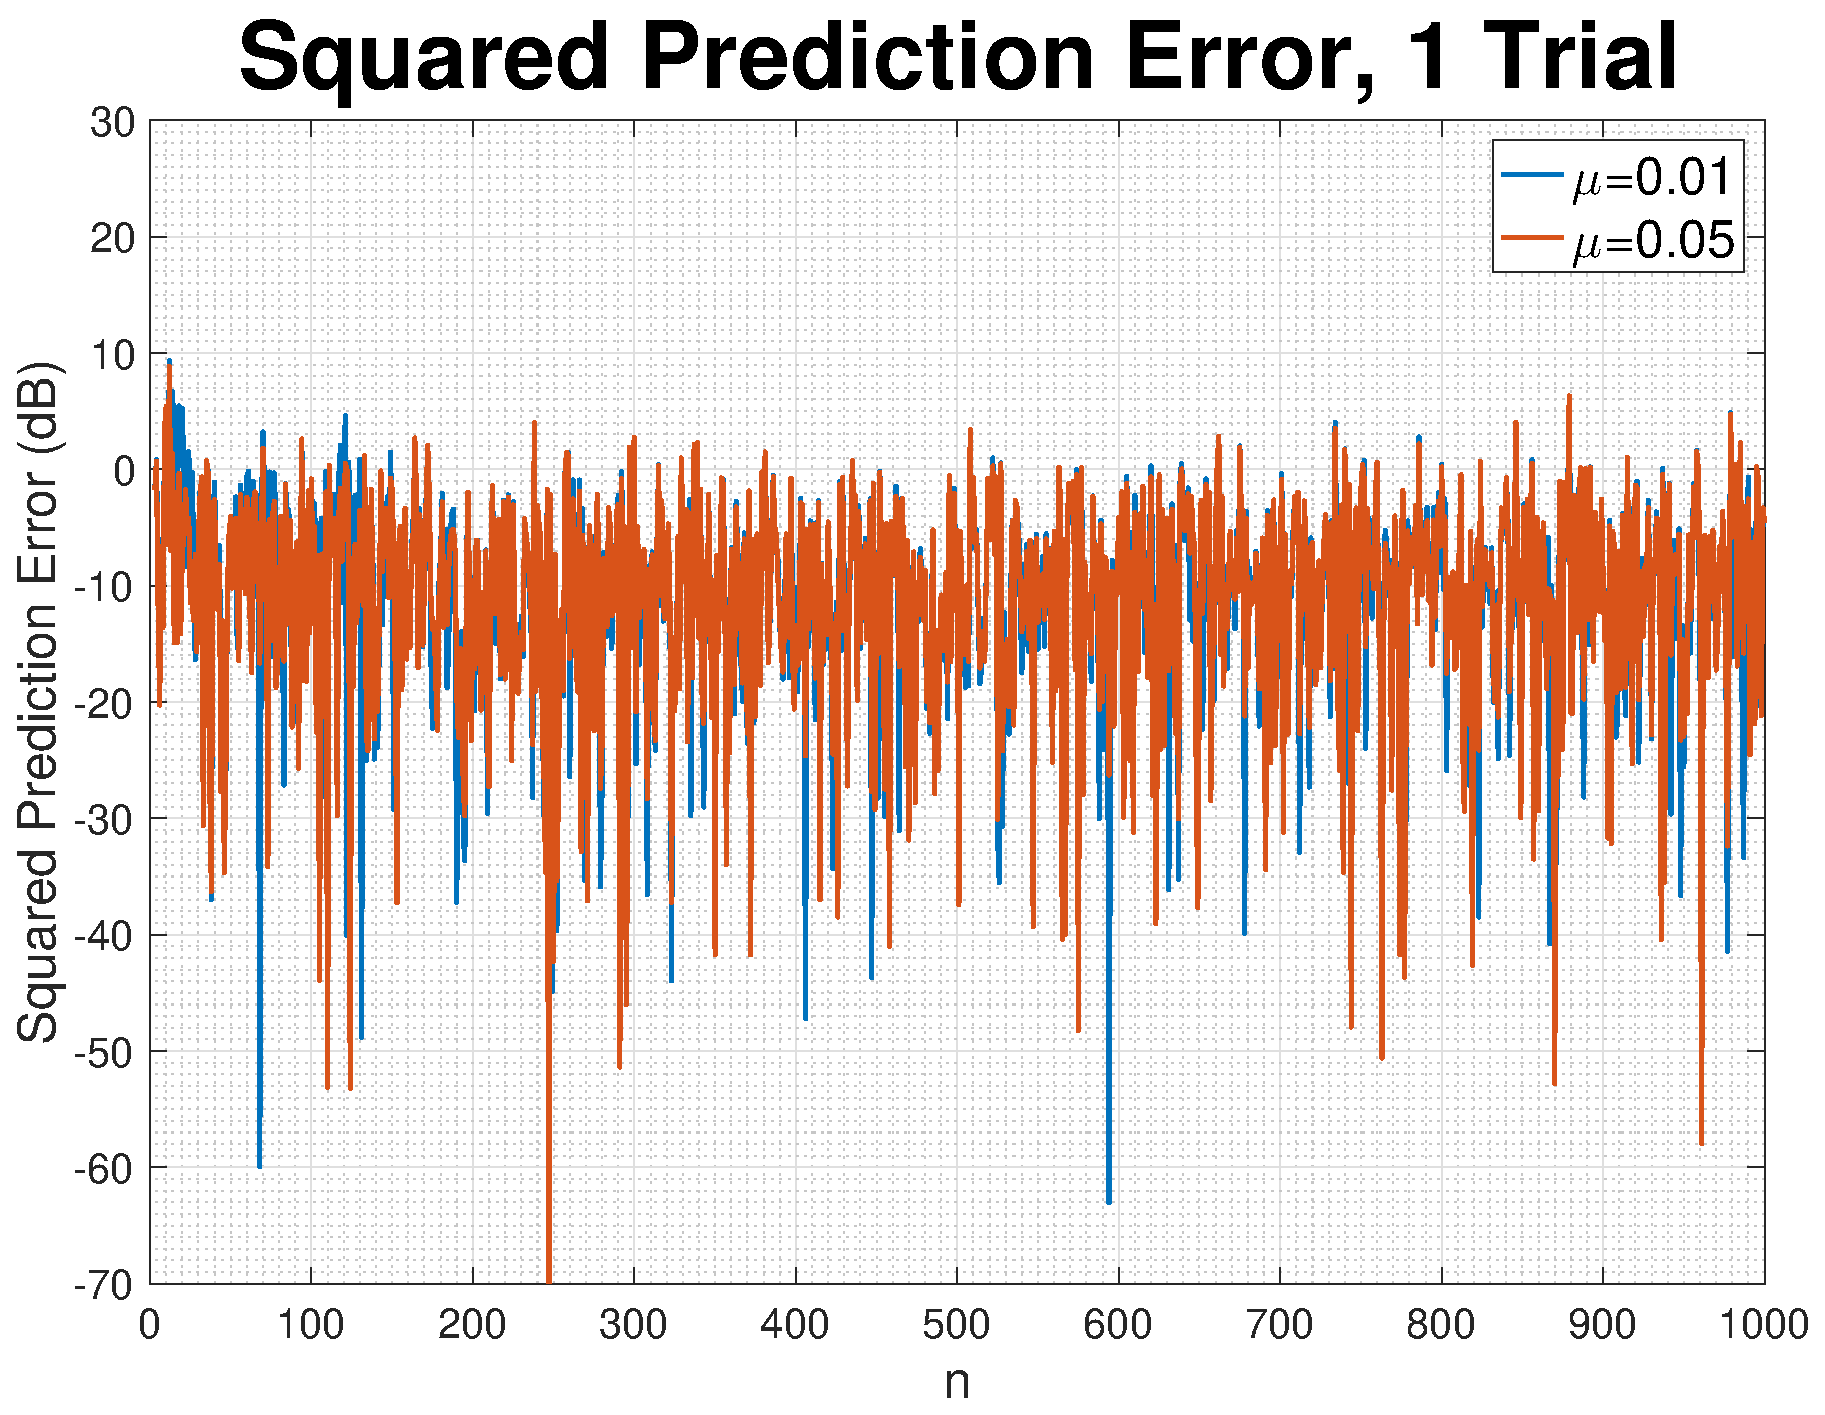
\includegraphics[width=0.32\textwidth]{part3/ar_lms_mu_1_realisation}
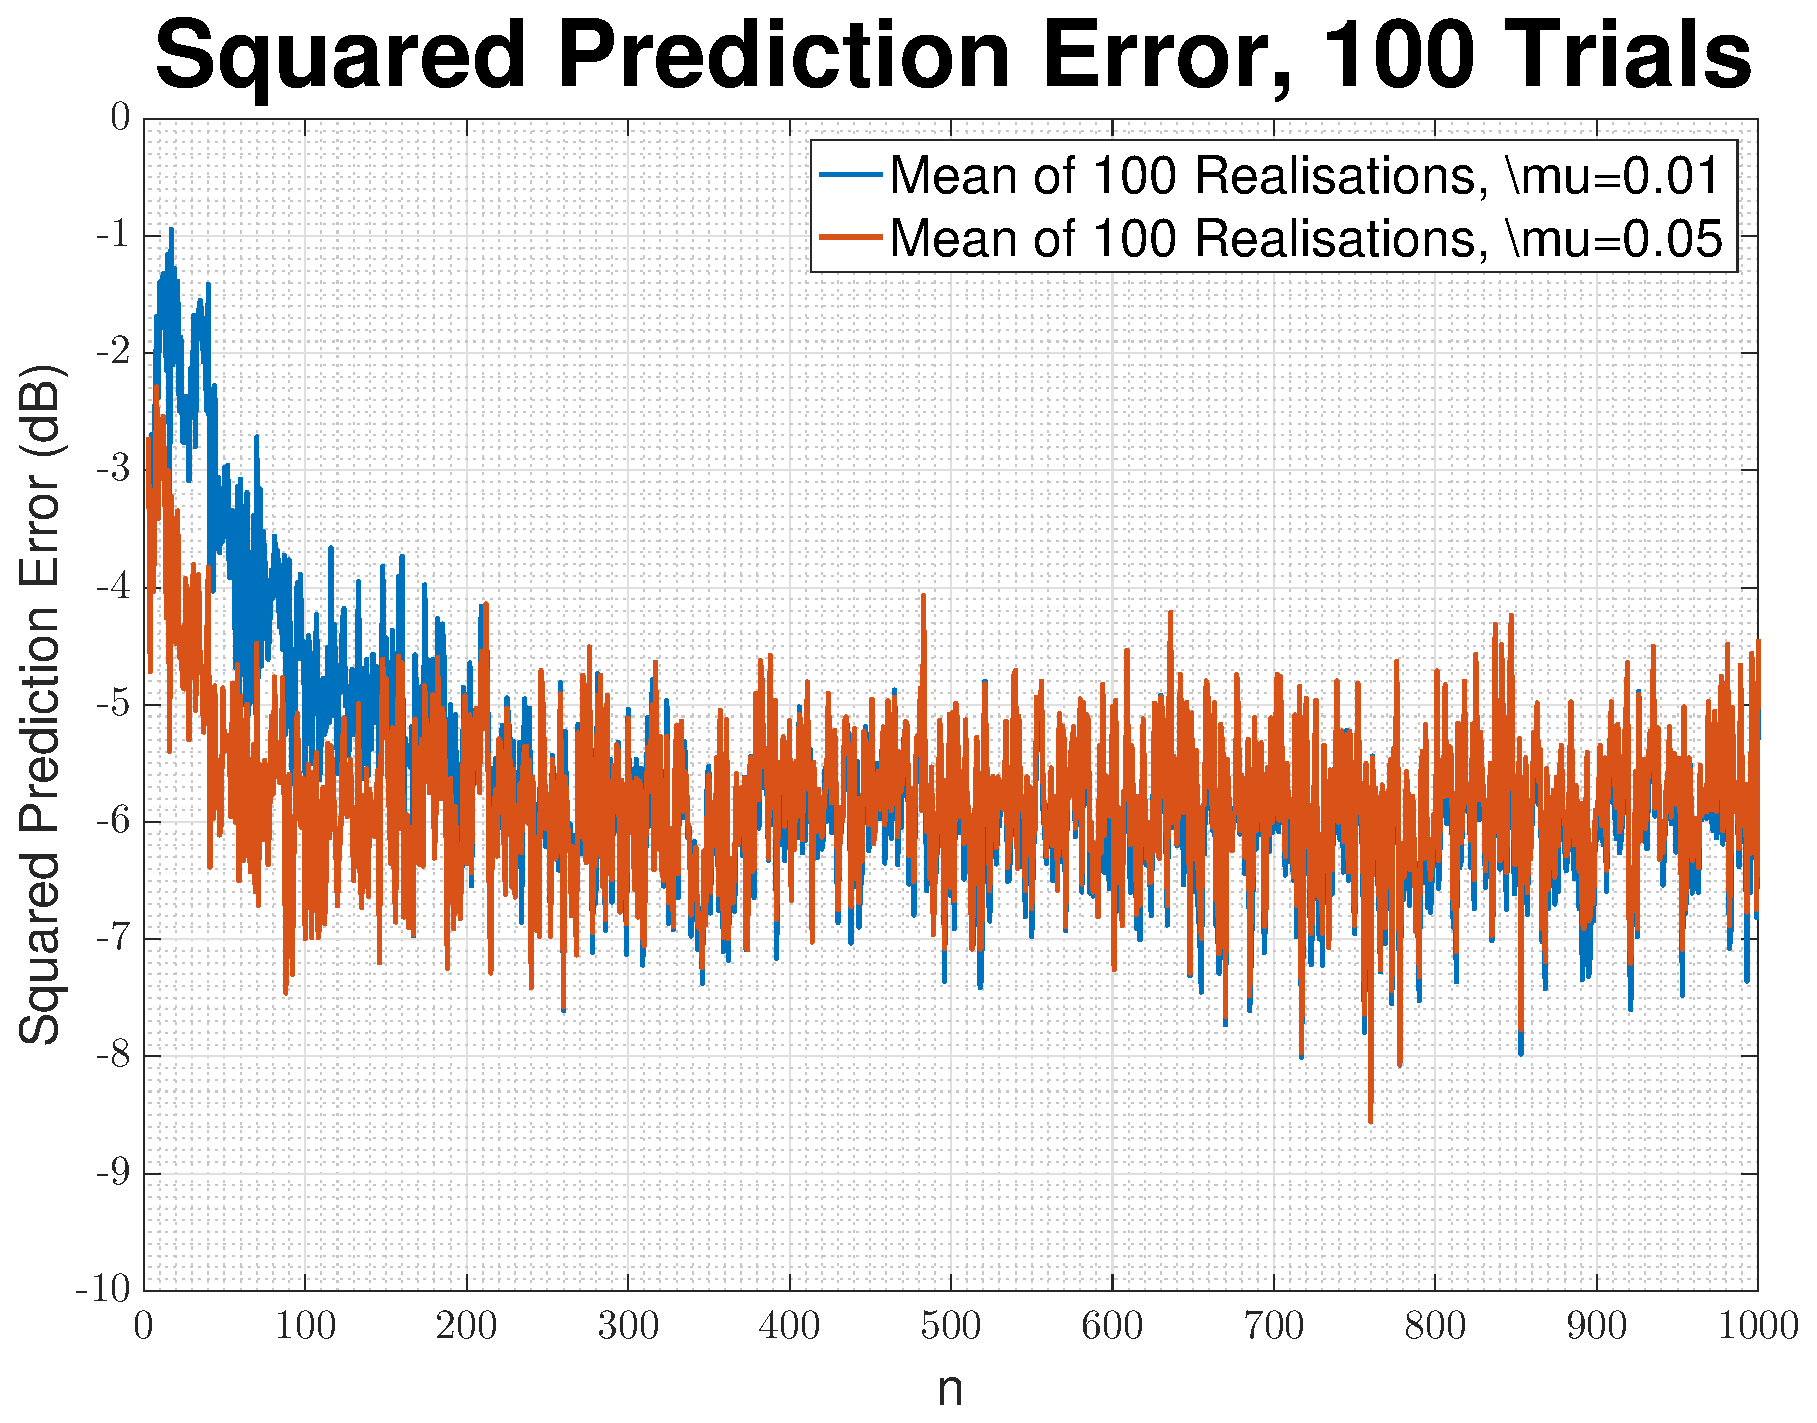
\includegraphics[width=0.32\textwidth]{part3/ar_lms_mu_100_realisation}
\caption{Analysis of Effects of Different Step Size on Convergence Speed of LMS Alogirthm}
\end{figure}

\begin{figure}[H]
\centering{}
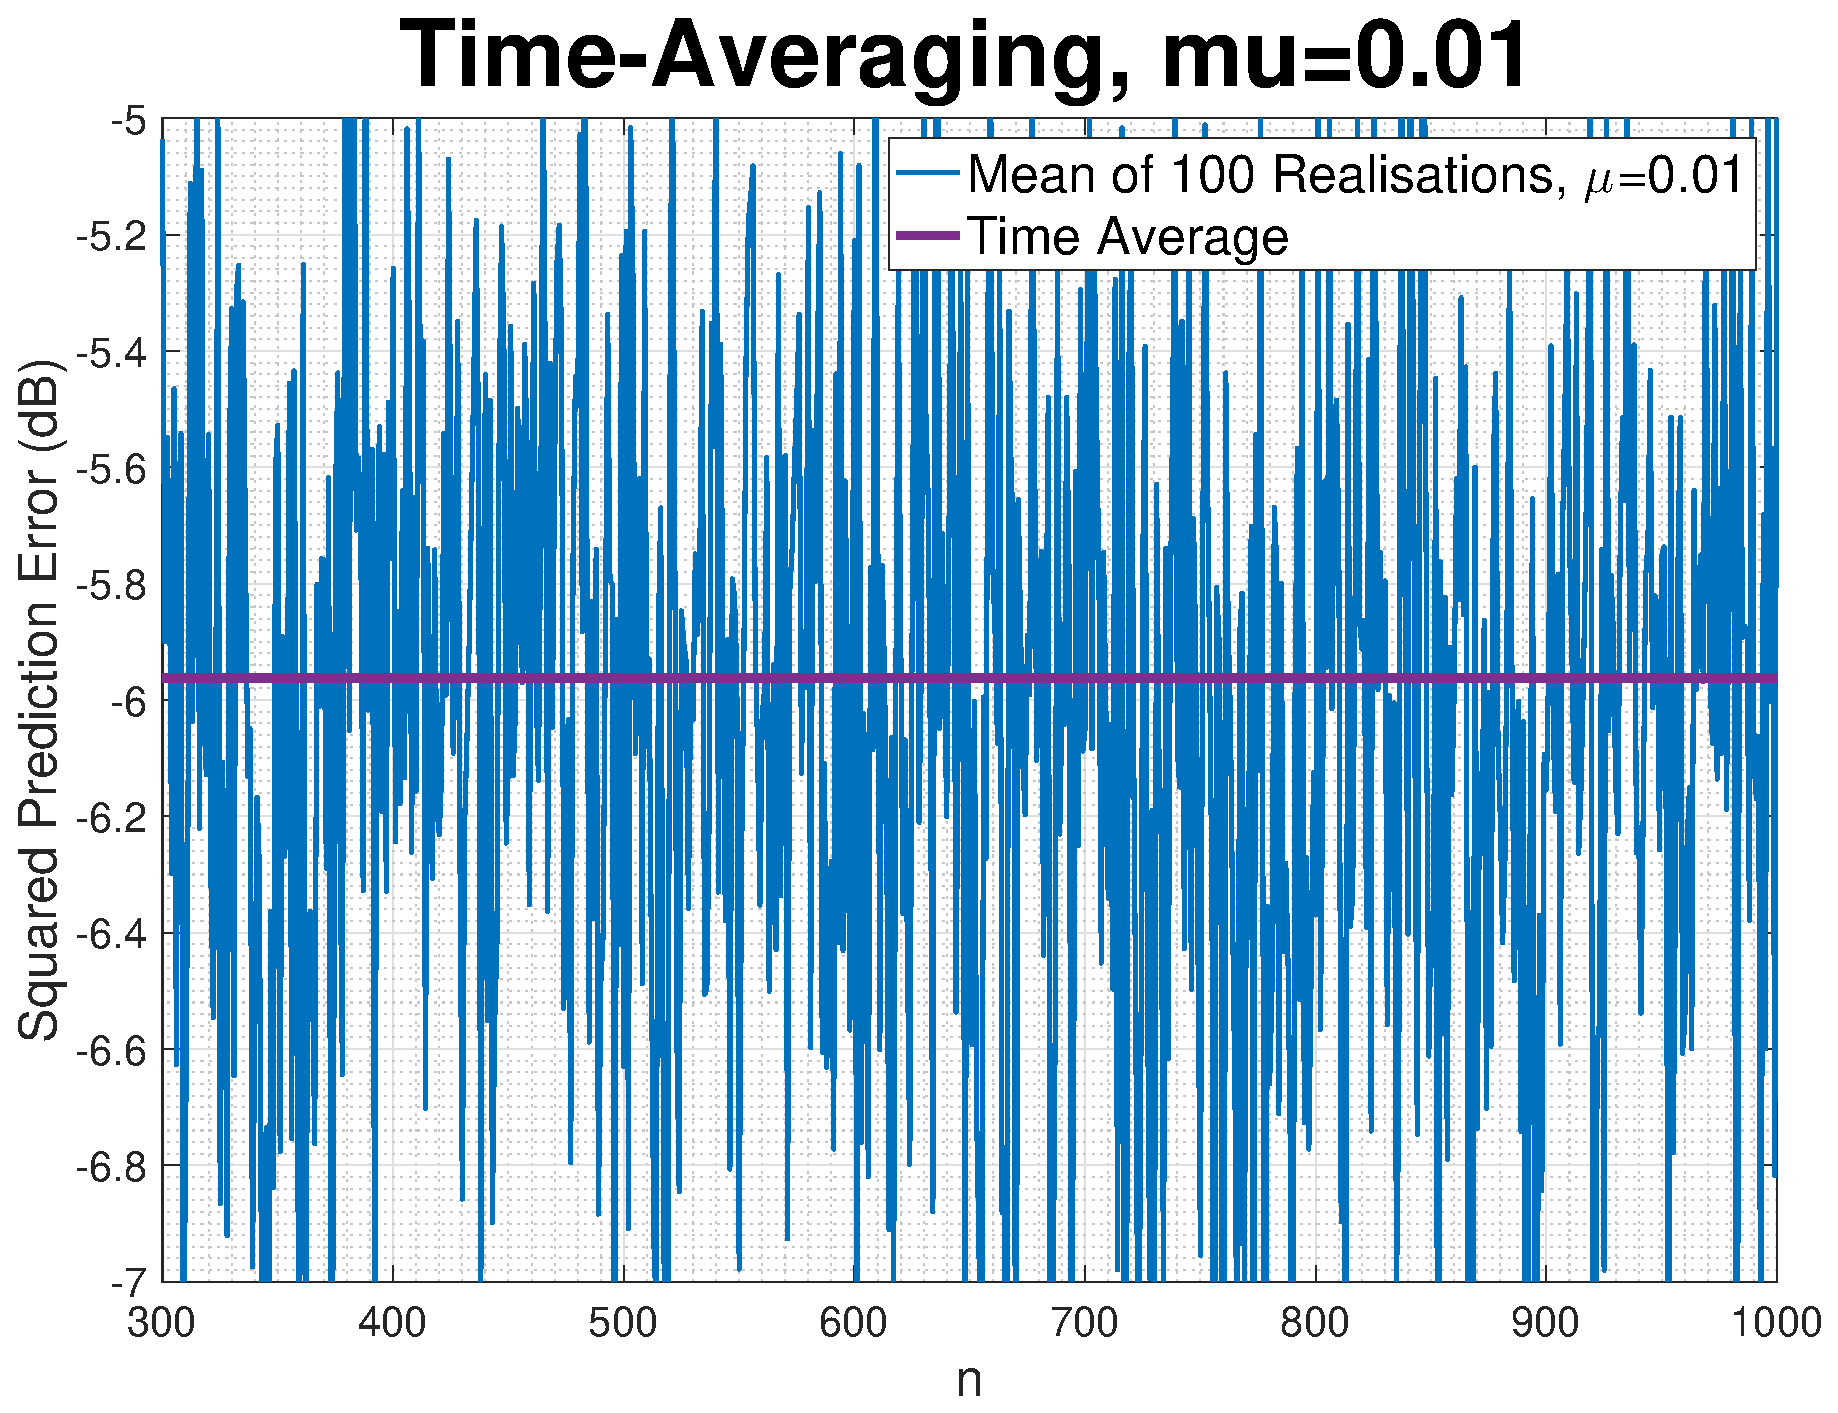
\includegraphics[width=0.32\textwidth]{part3/time_average_mu_01}
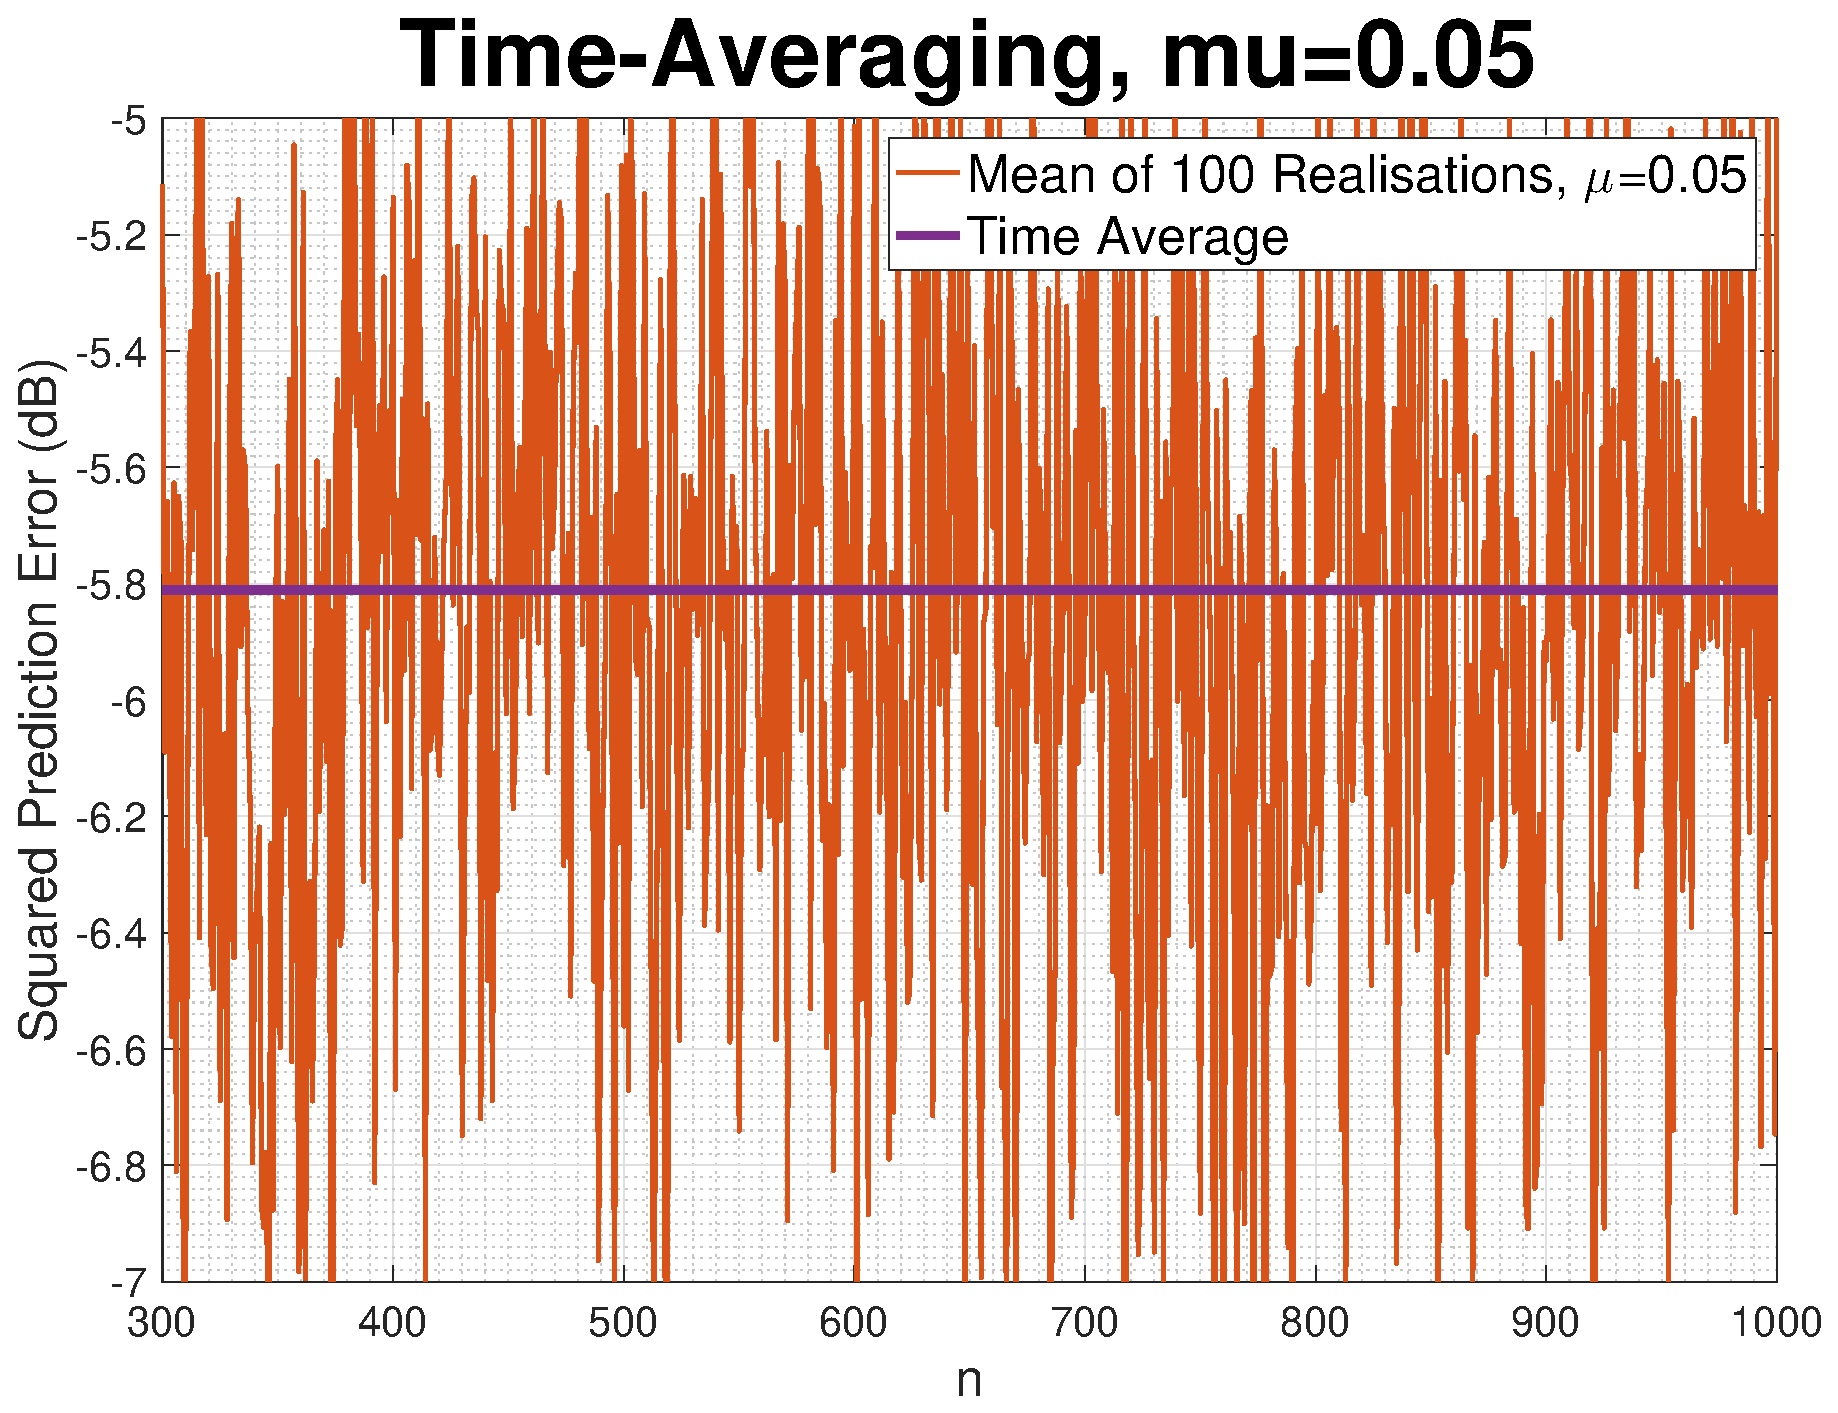
\includegraphics[width=0.32\textwidth]{part3/time_average_mu_05}
\caption{Time-Average of Steady State Error for $\mu=0.01$ and $\mu=0.05$}
\end{figure}


\begin{figure}[H]
\centering{}
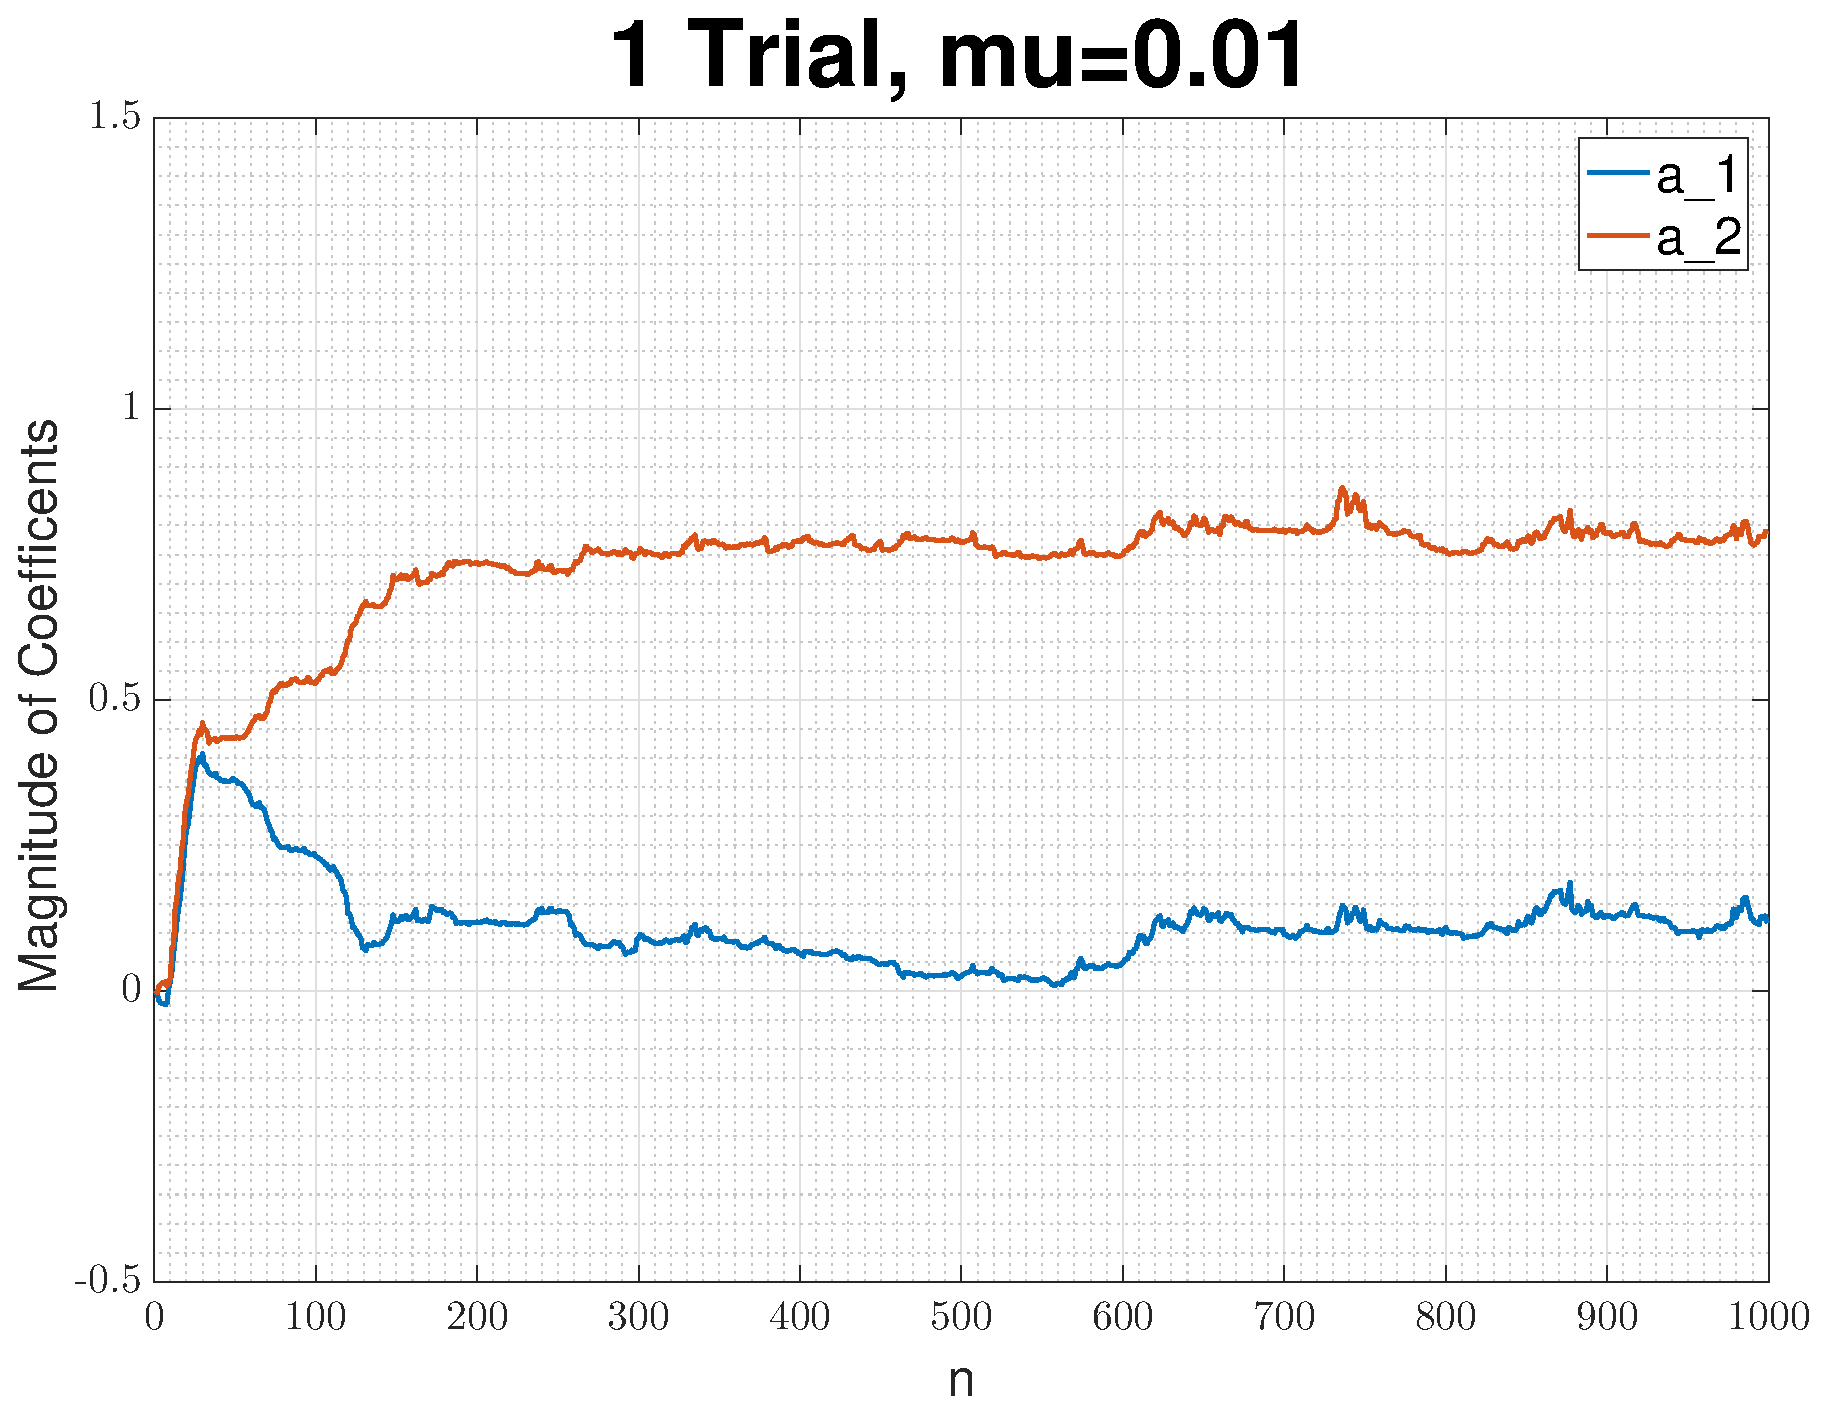
\includegraphics[width=0.32\textwidth]{part3/ar_coefficients_evolution_mu_01_1_trial}
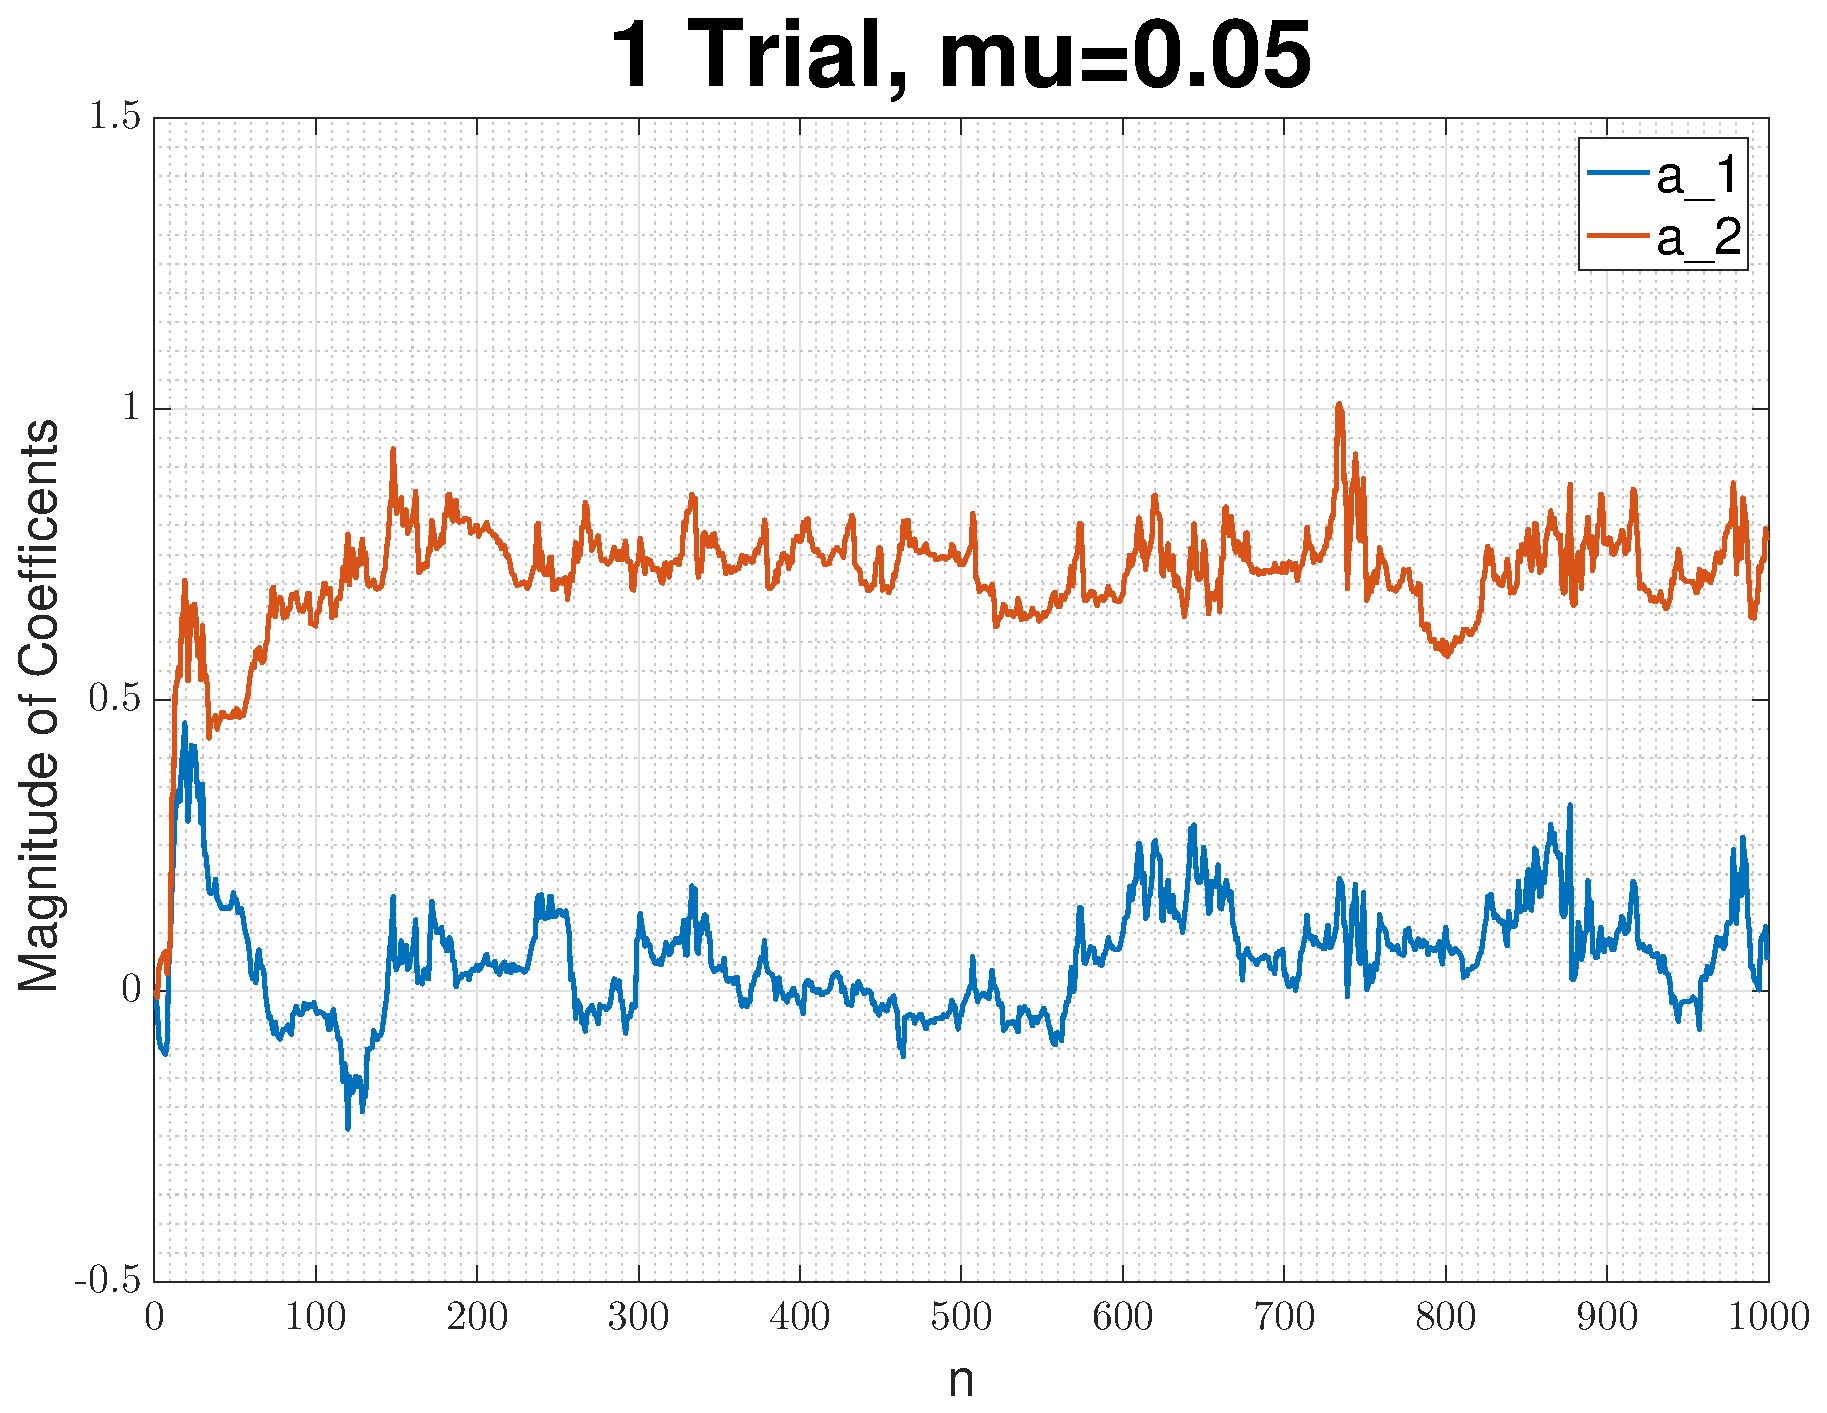
\includegraphics[width=0.32\textwidth]{part3/ar_coefficients_evolution_mu_05_1_trial}
\caption{Evolution of Coefficients for 1 Trial, for $\mu=0.01$ and $\mu=0.05$}
\end{figure}


\begin{figure}[H]
\centering{}
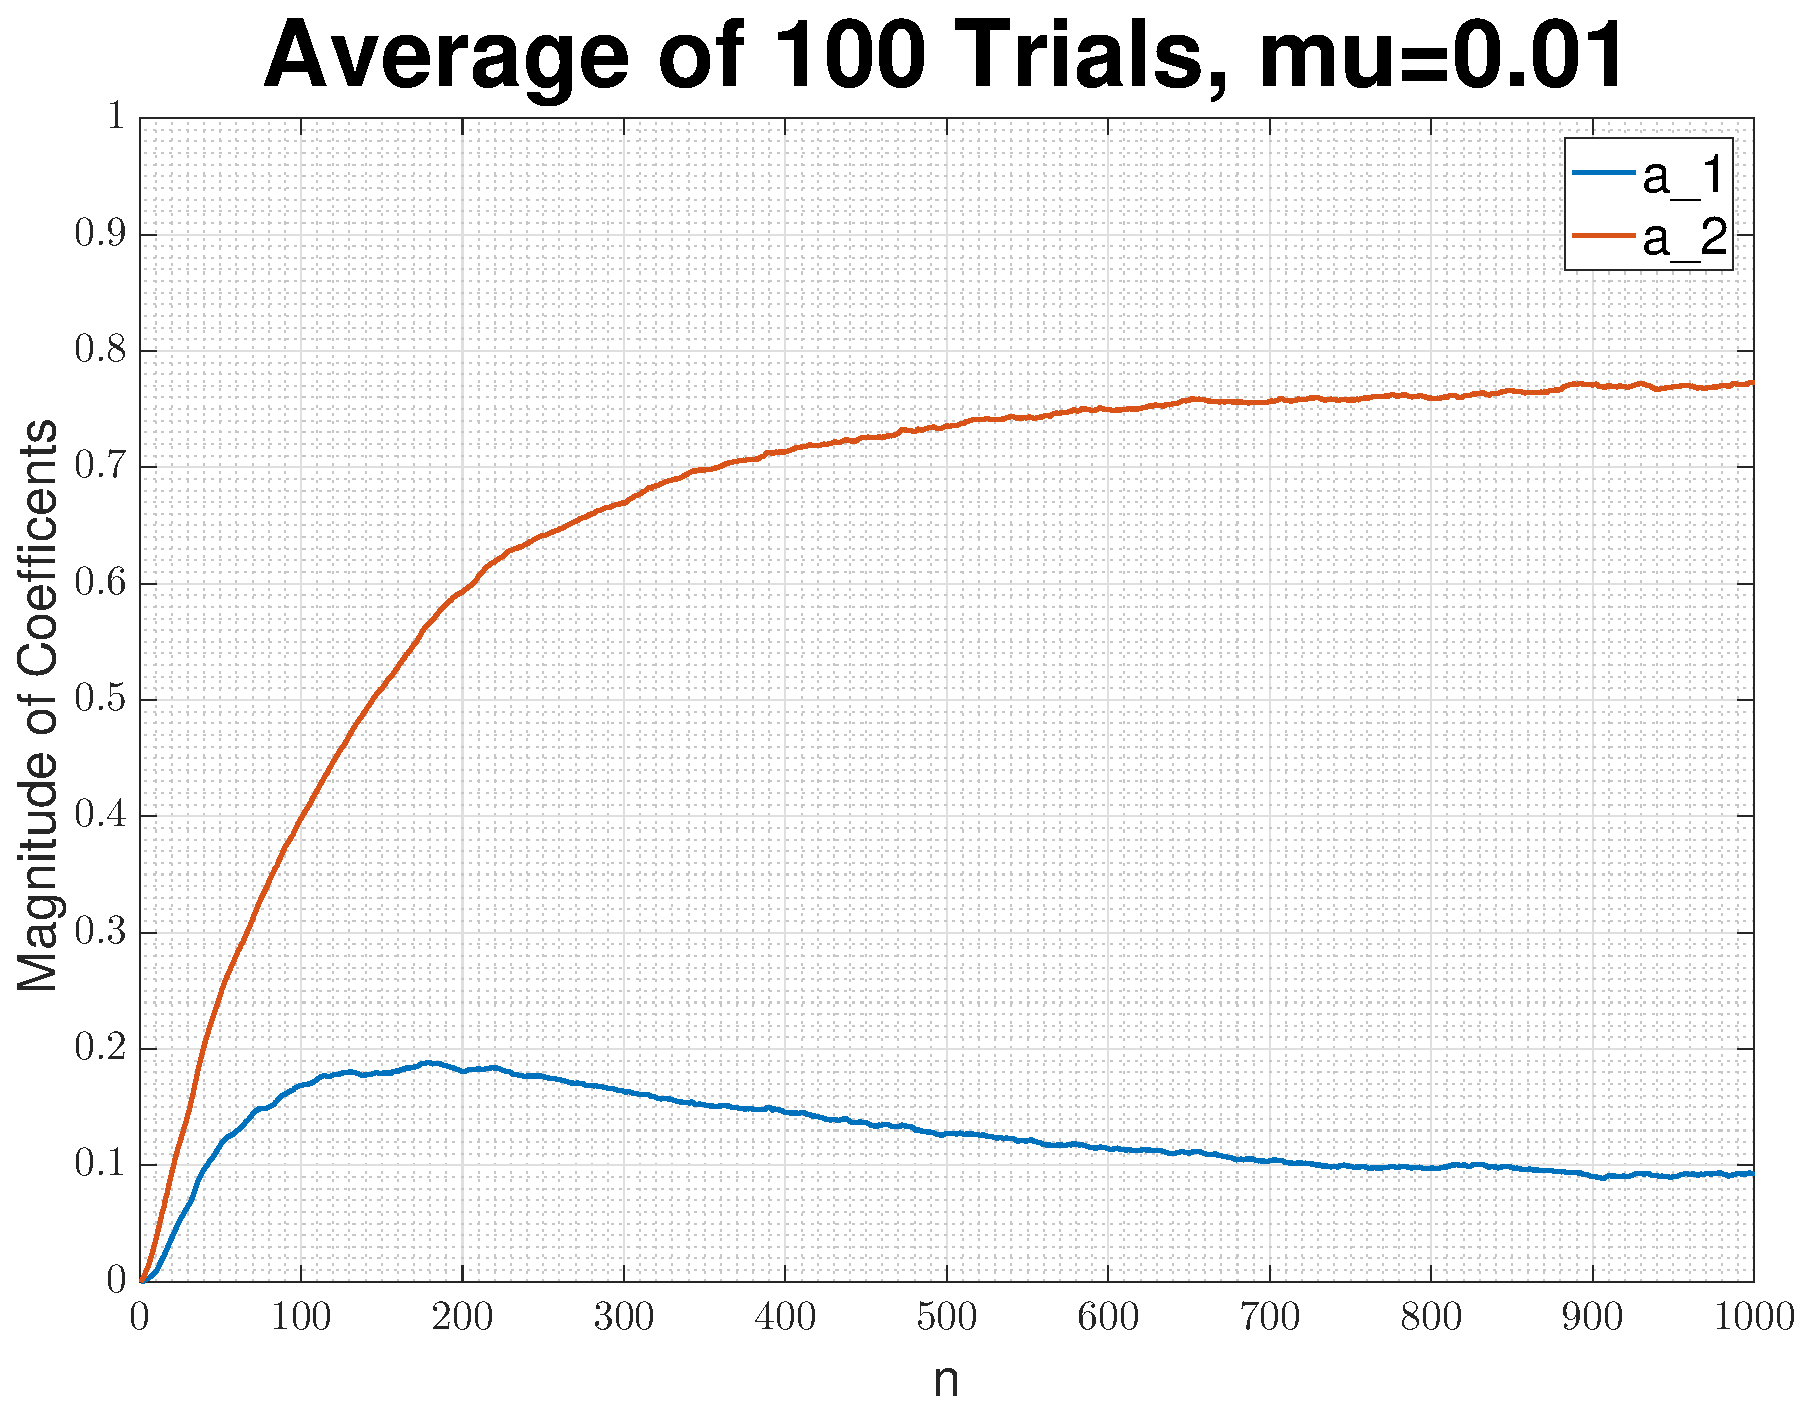
\includegraphics[width=0.32\textwidth]{part3/ar_coefficients_evolution_mu_01}
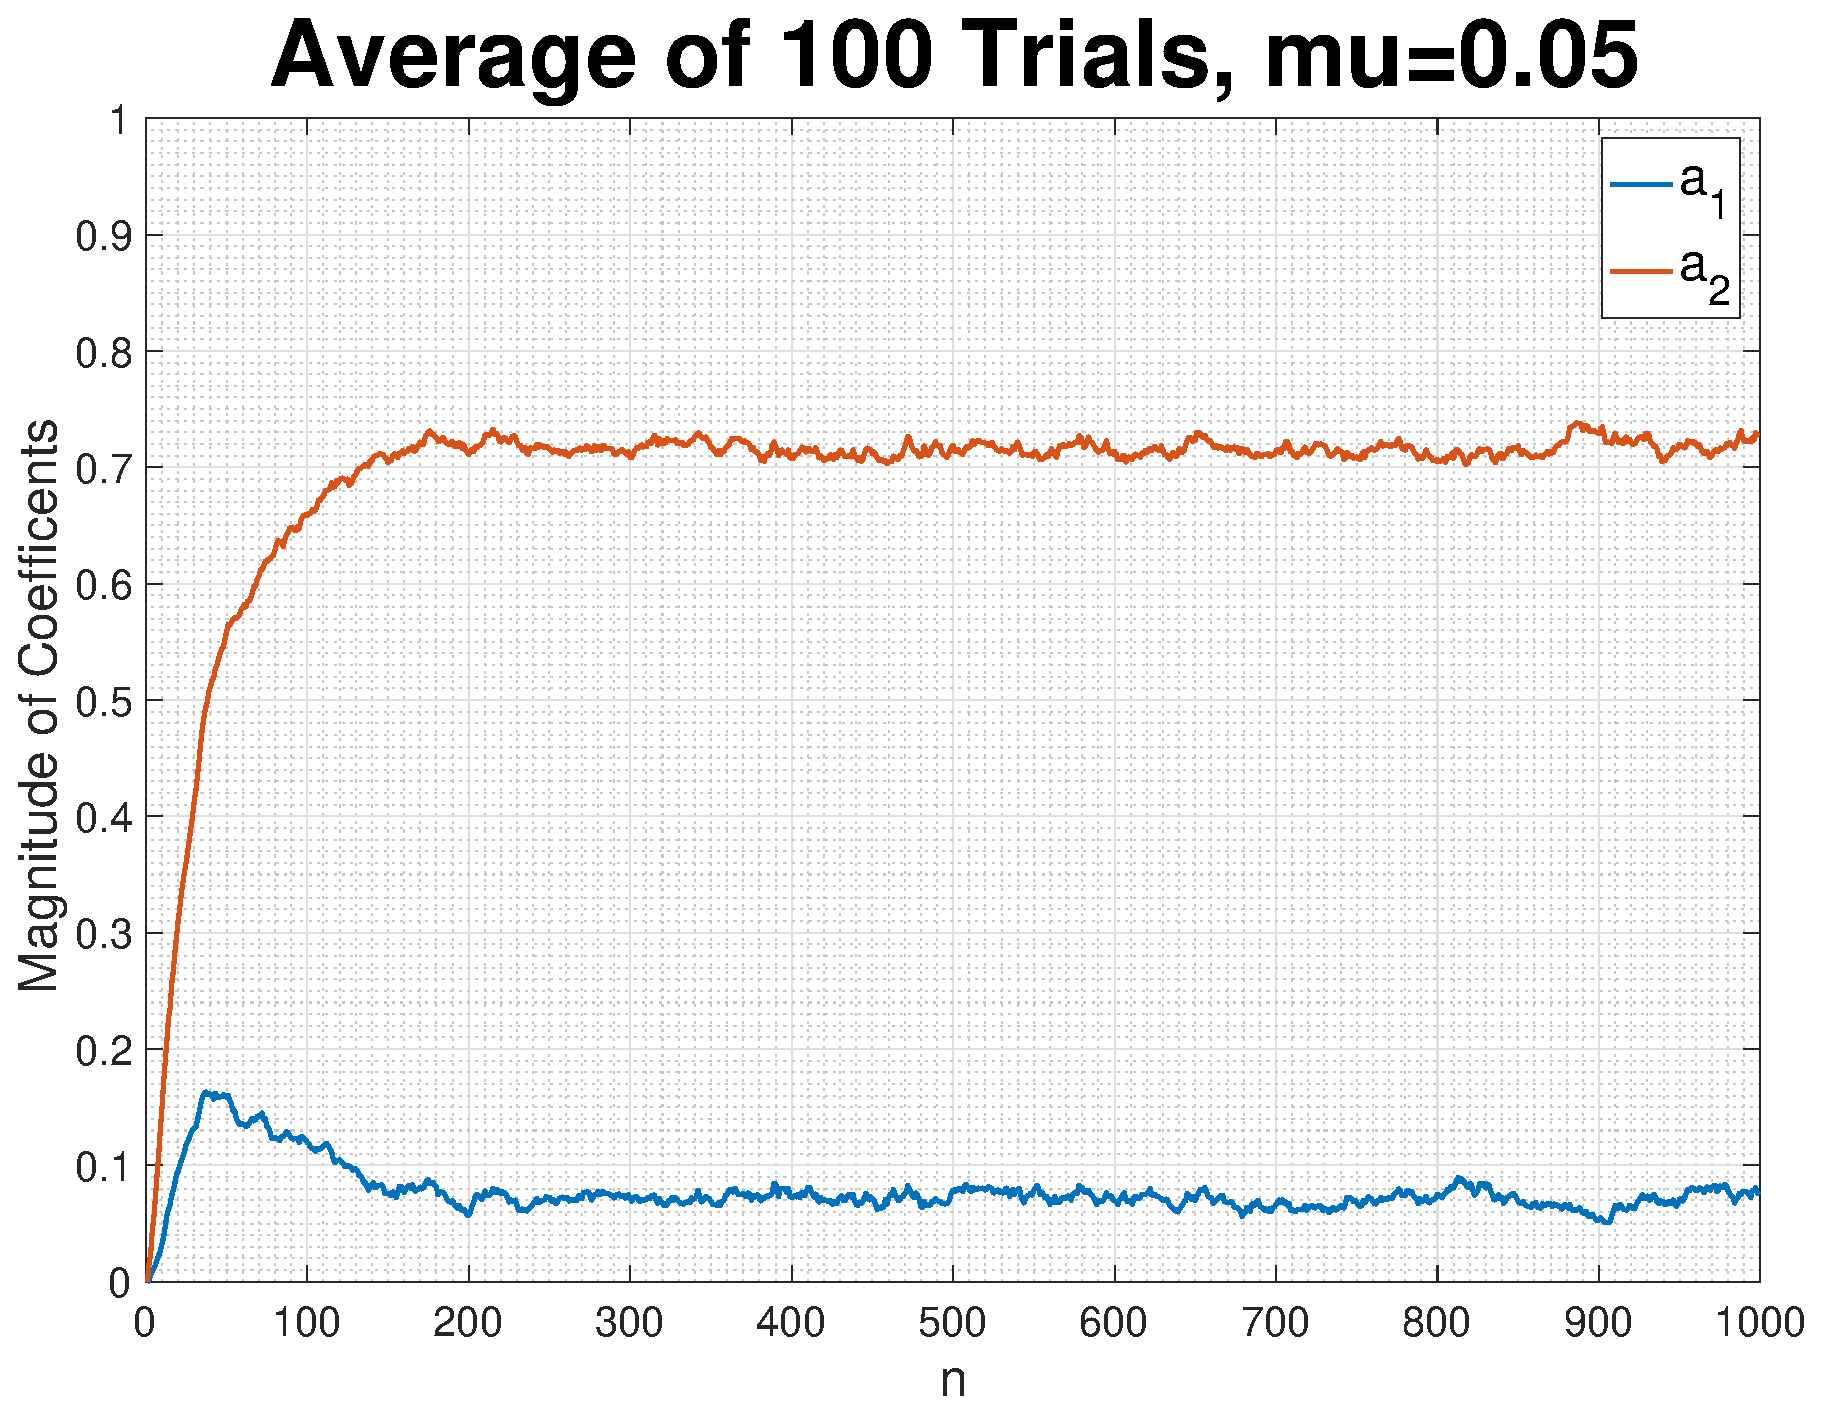
\includegraphics[width=0.32\textwidth]{part3/ar_coefficients_evolution_mu_05}
\caption{Evolution of Coefficients for 100 Trial, for $\mu=0.01$ and $\mu=0.05$}
\end{figure}

\begin{figure}[H]
\centering{}
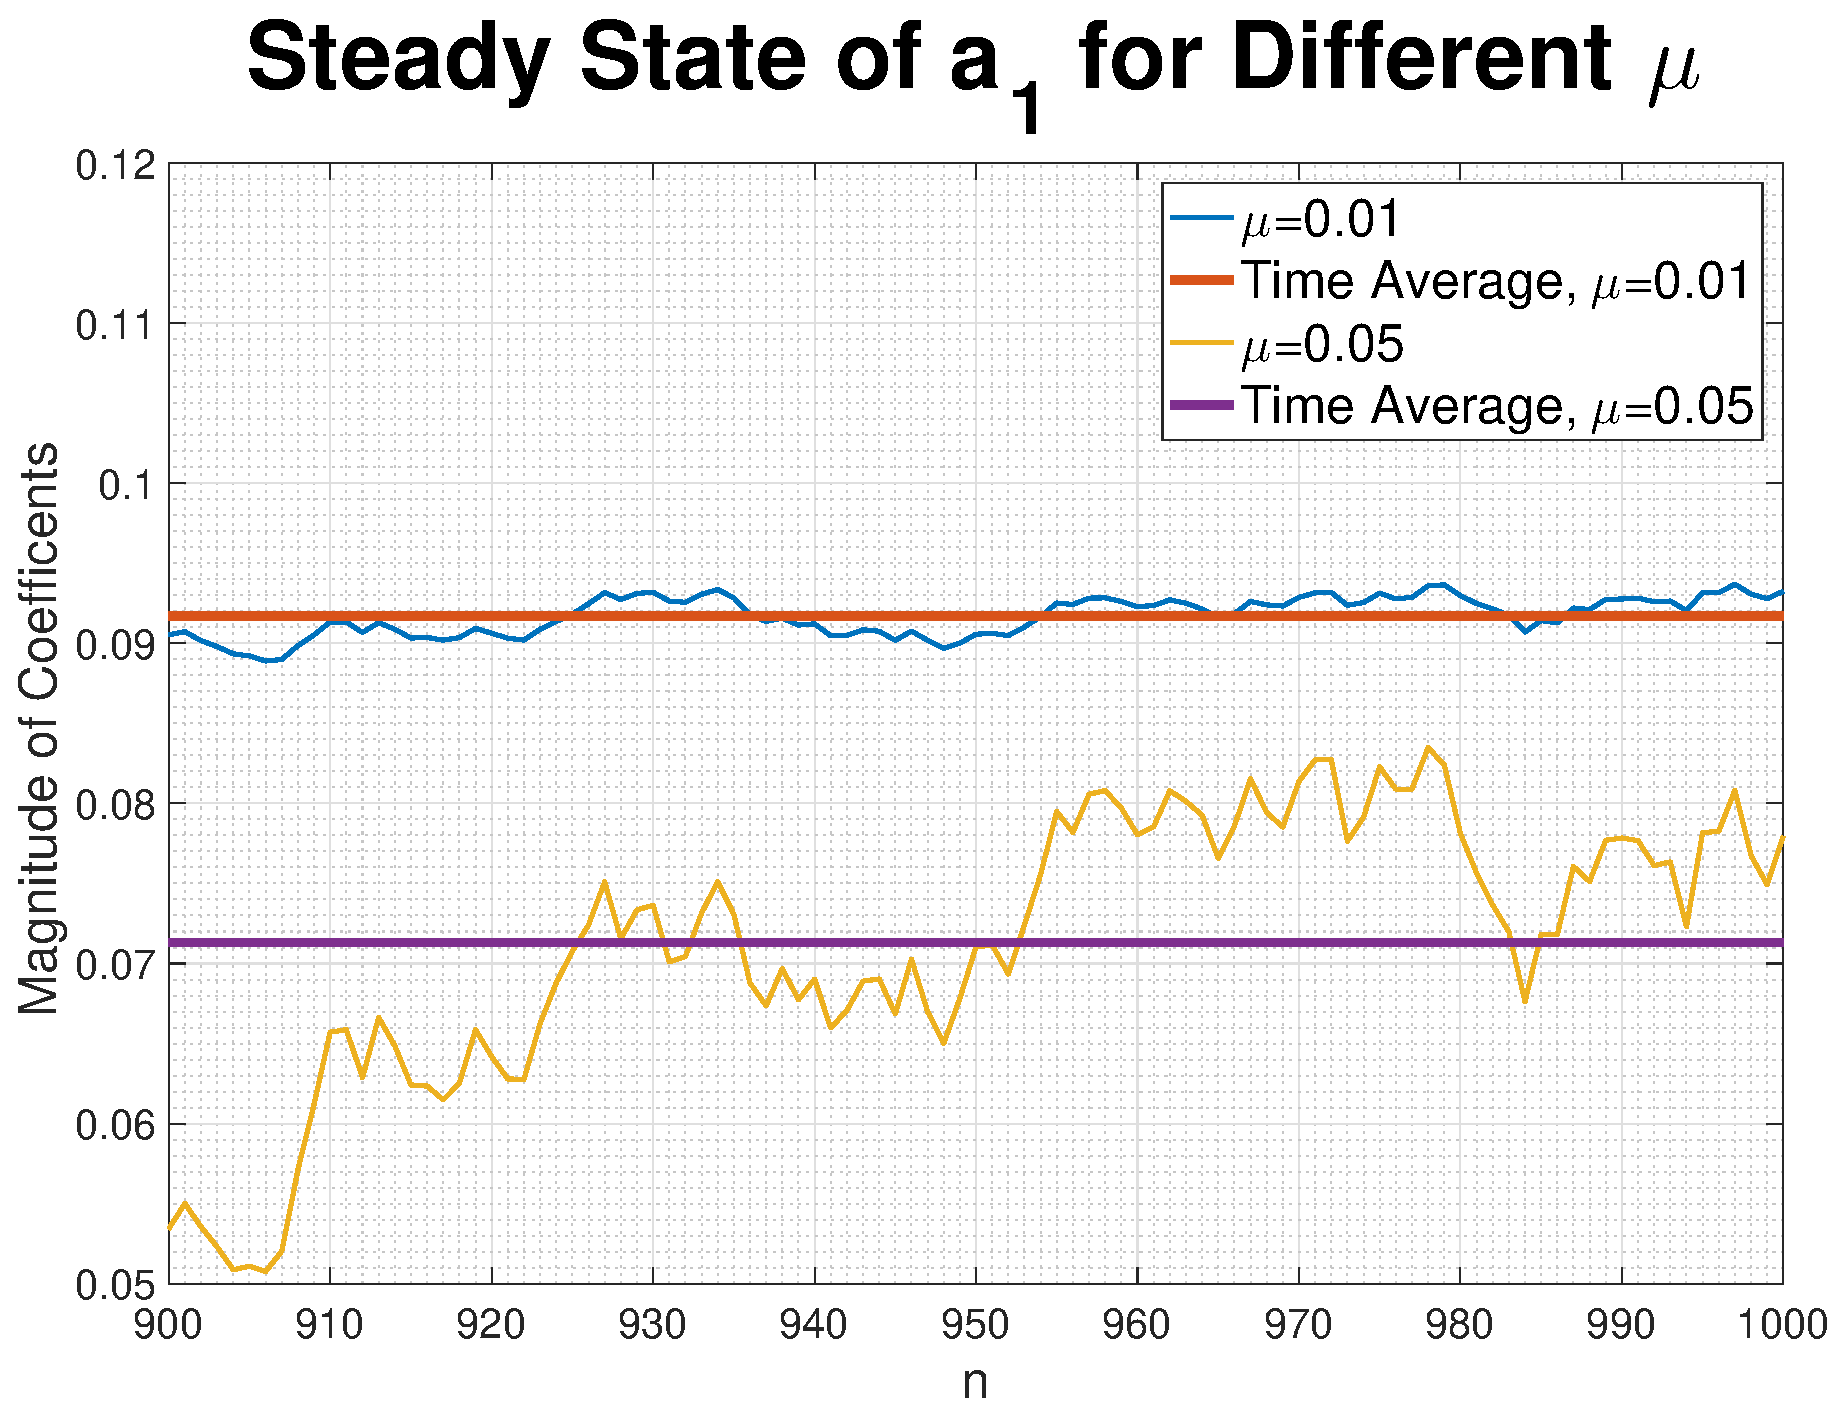
\includegraphics[width=0.32\textwidth]{part3/steady_state_ar_coeff_1}
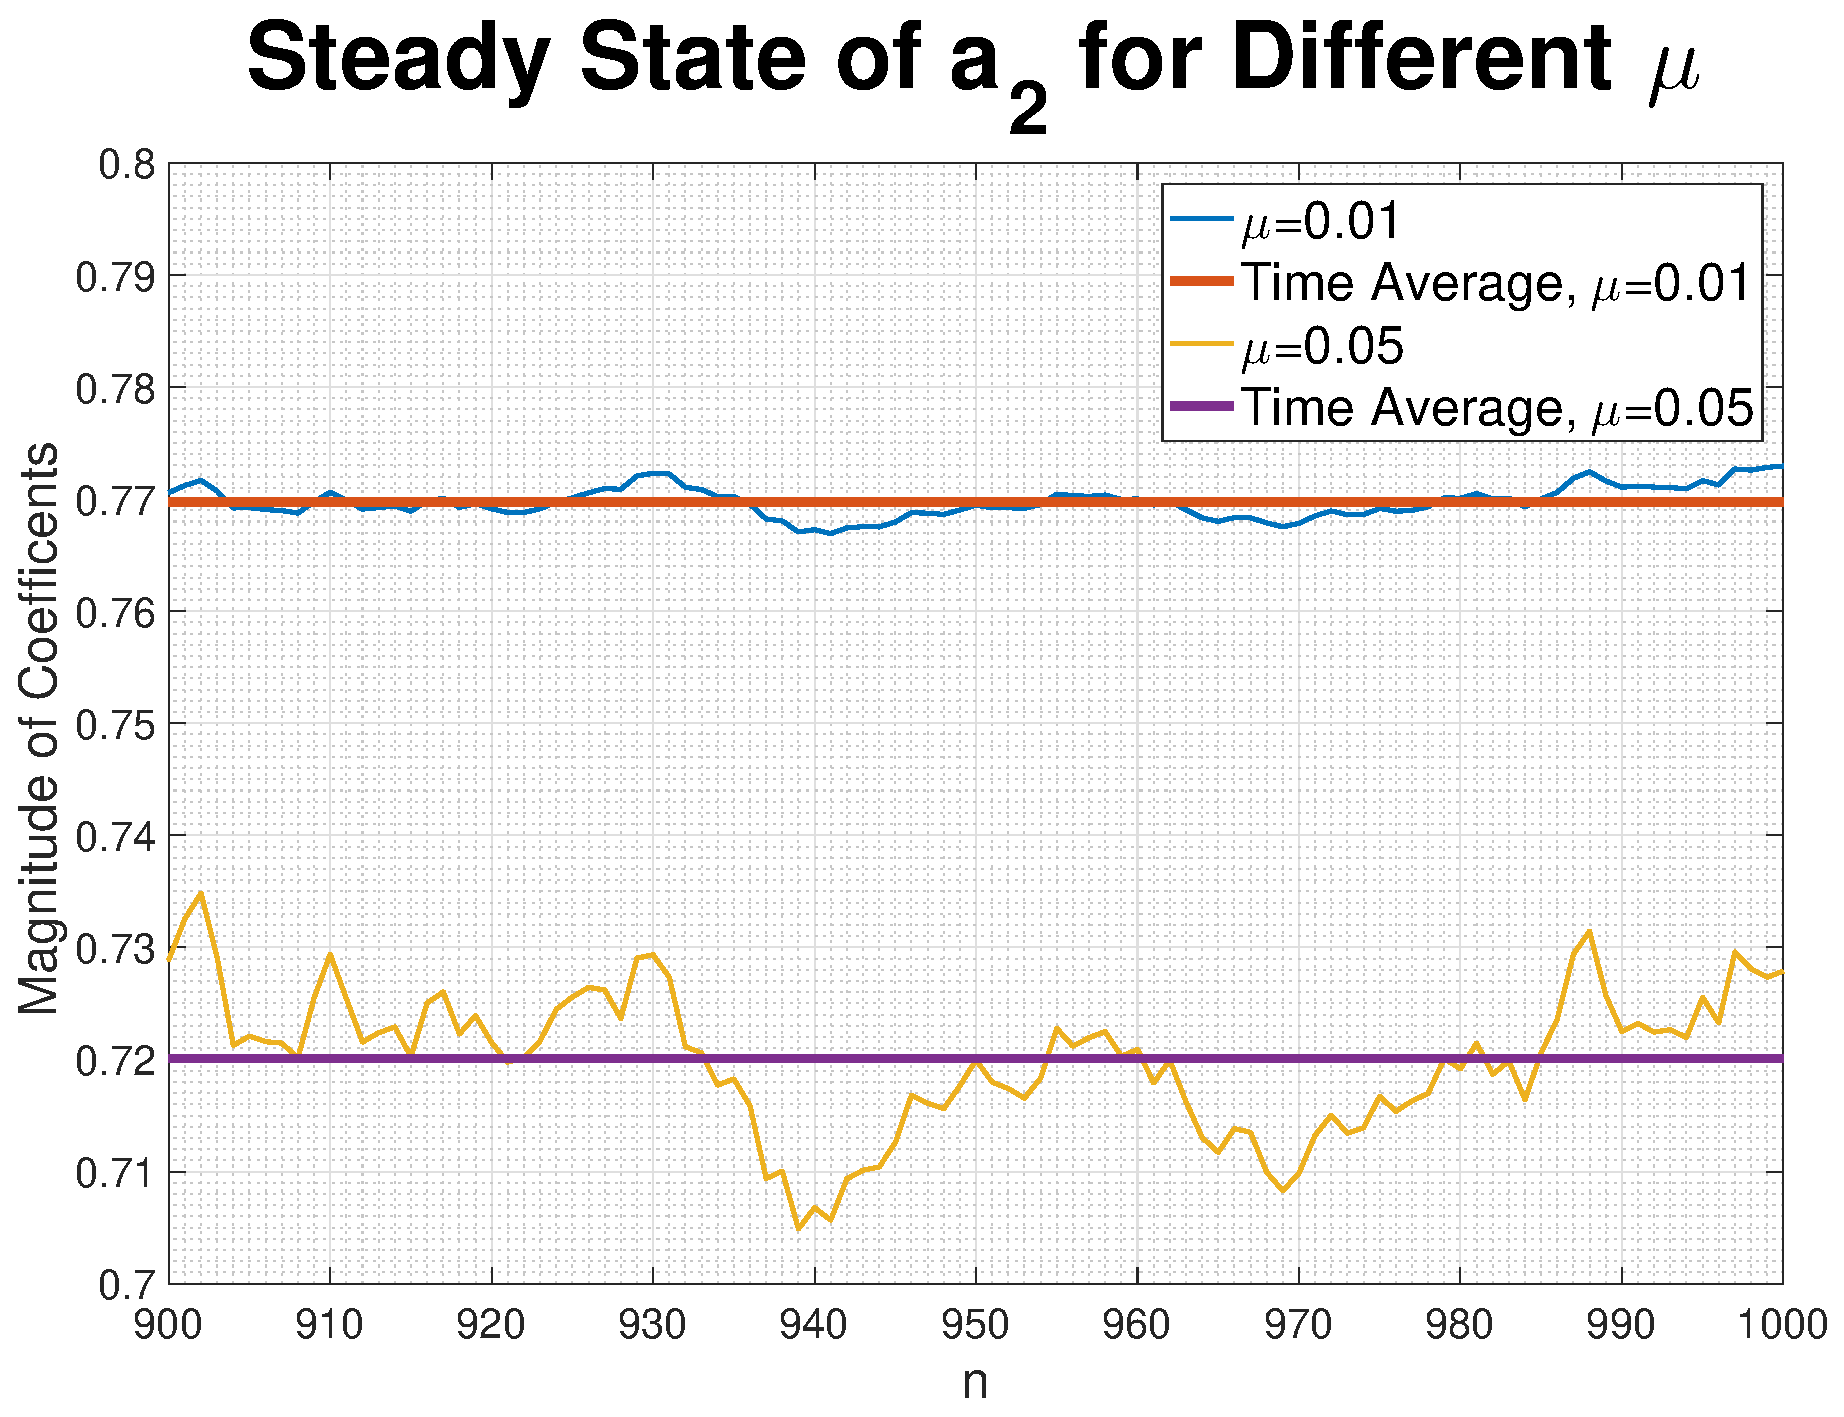
\includegraphics[width=0.32\textwidth]{part3/steady_state_ar_coeff_2}
\caption{Steady State Values of Coefficients $a_1$ and $a_2$, for $\mu=0.01$ and $\mu=0.05$}
\end{figure}

\begin{figure}[H]
\centering{}
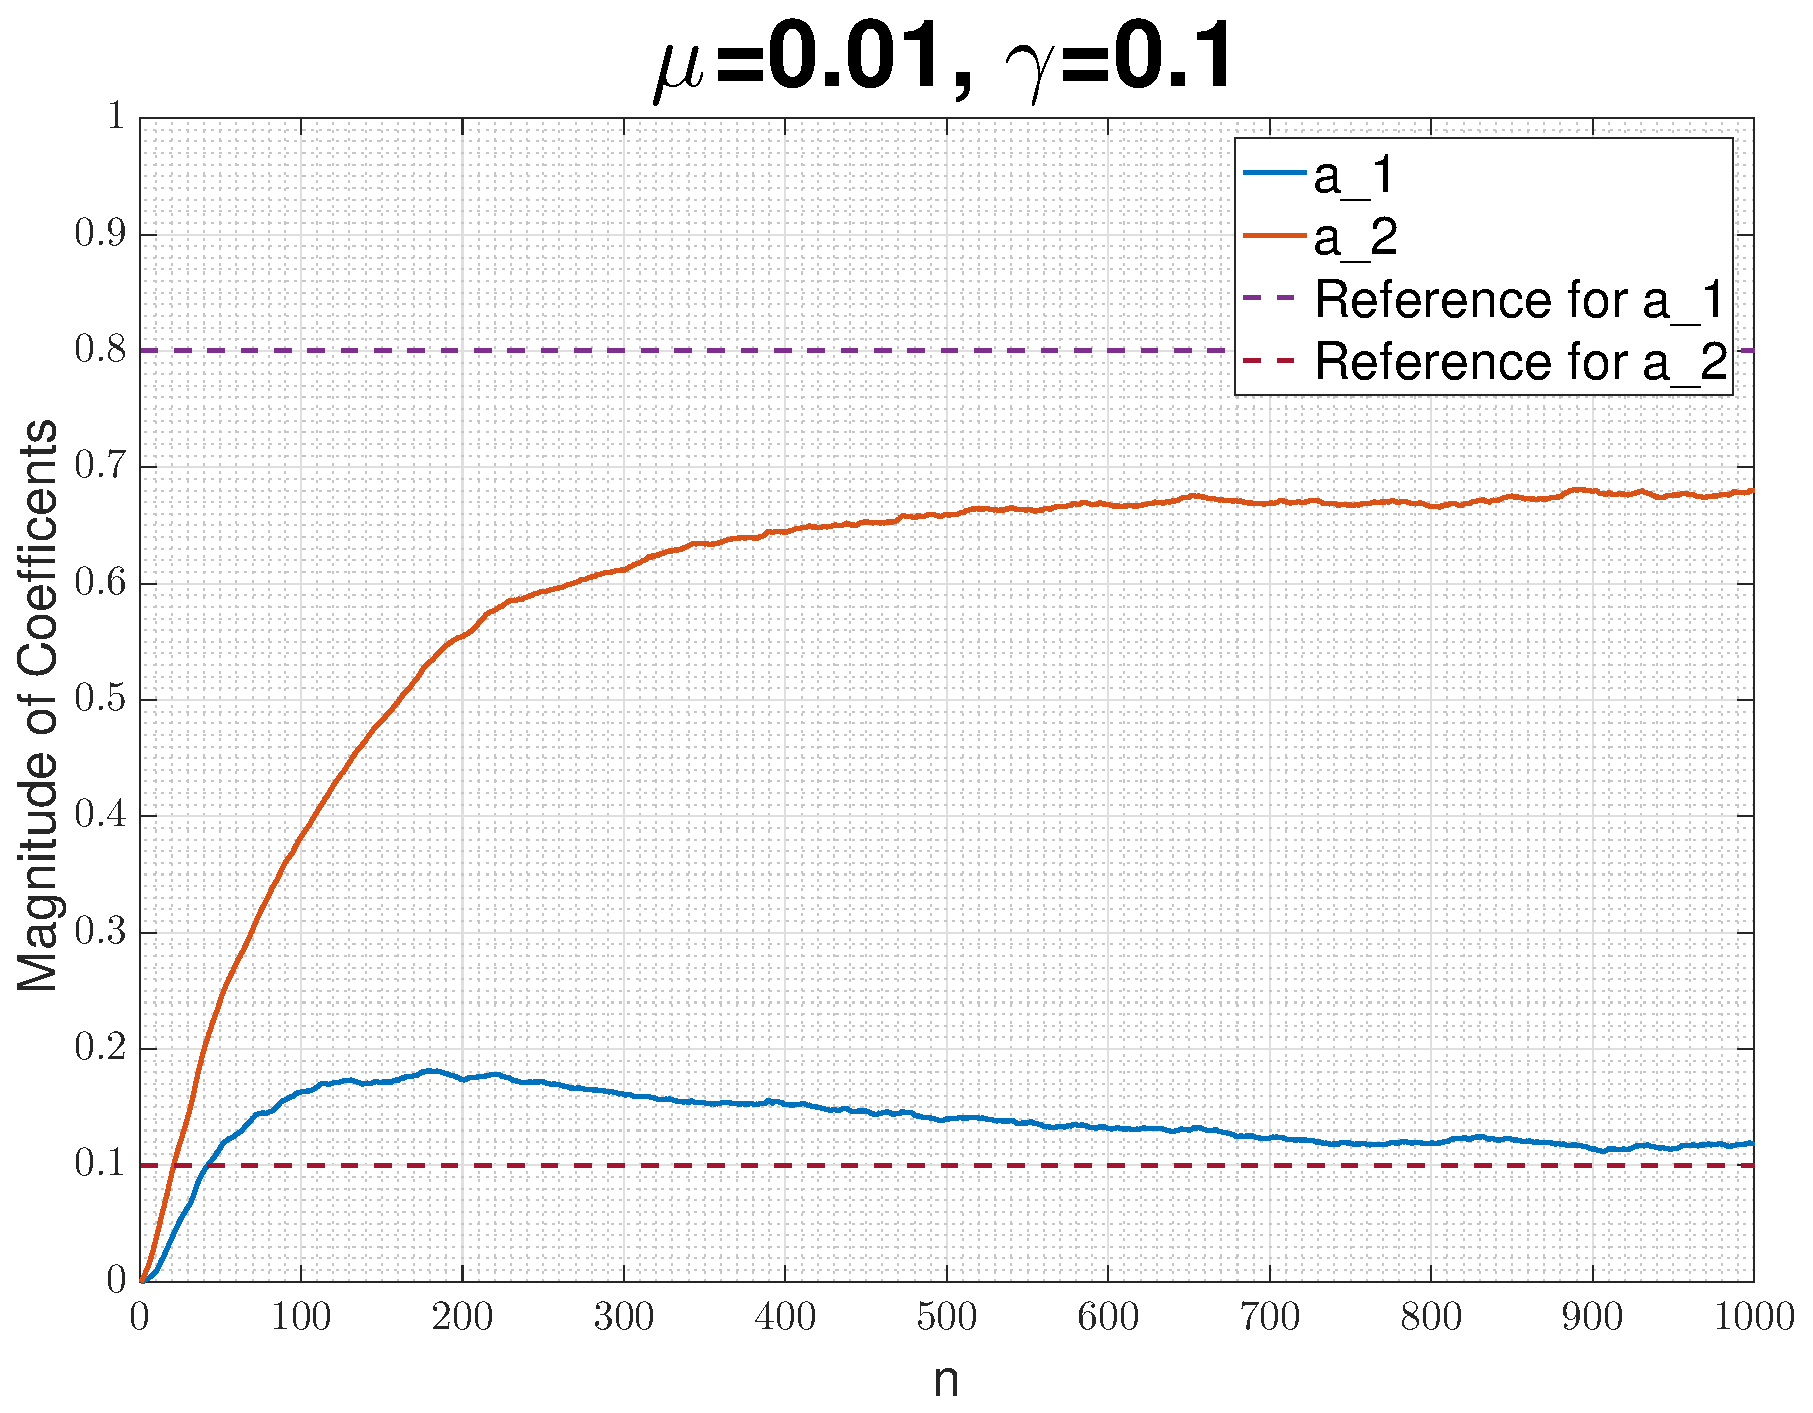
\includegraphics[width=0.32\textwidth]{part3/leaky_mu_01_gamma_01}
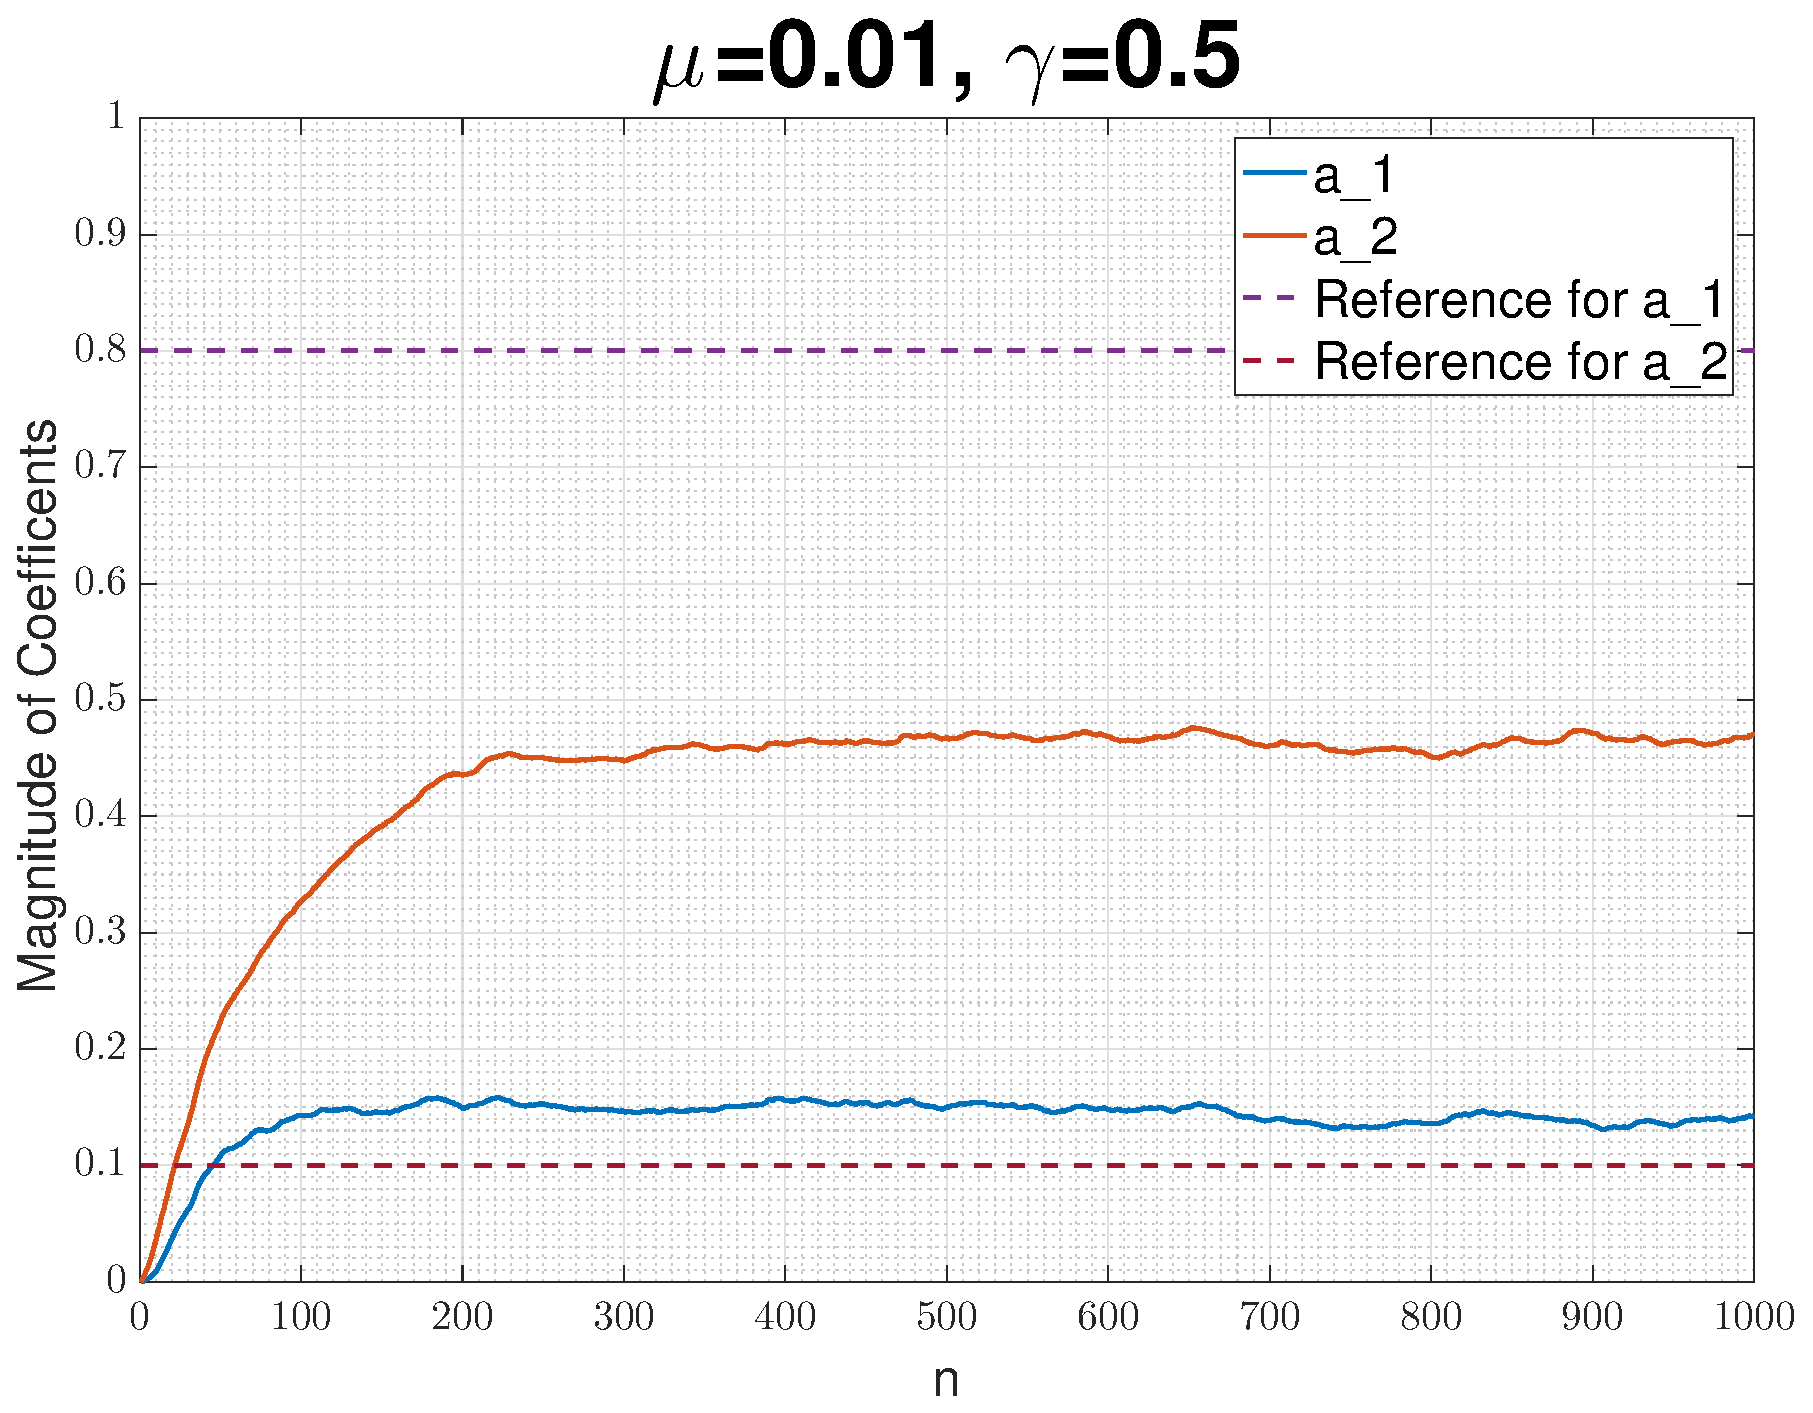
\includegraphics[width=0.32\textwidth]{part3/leaky_mu_01_gamma_05}
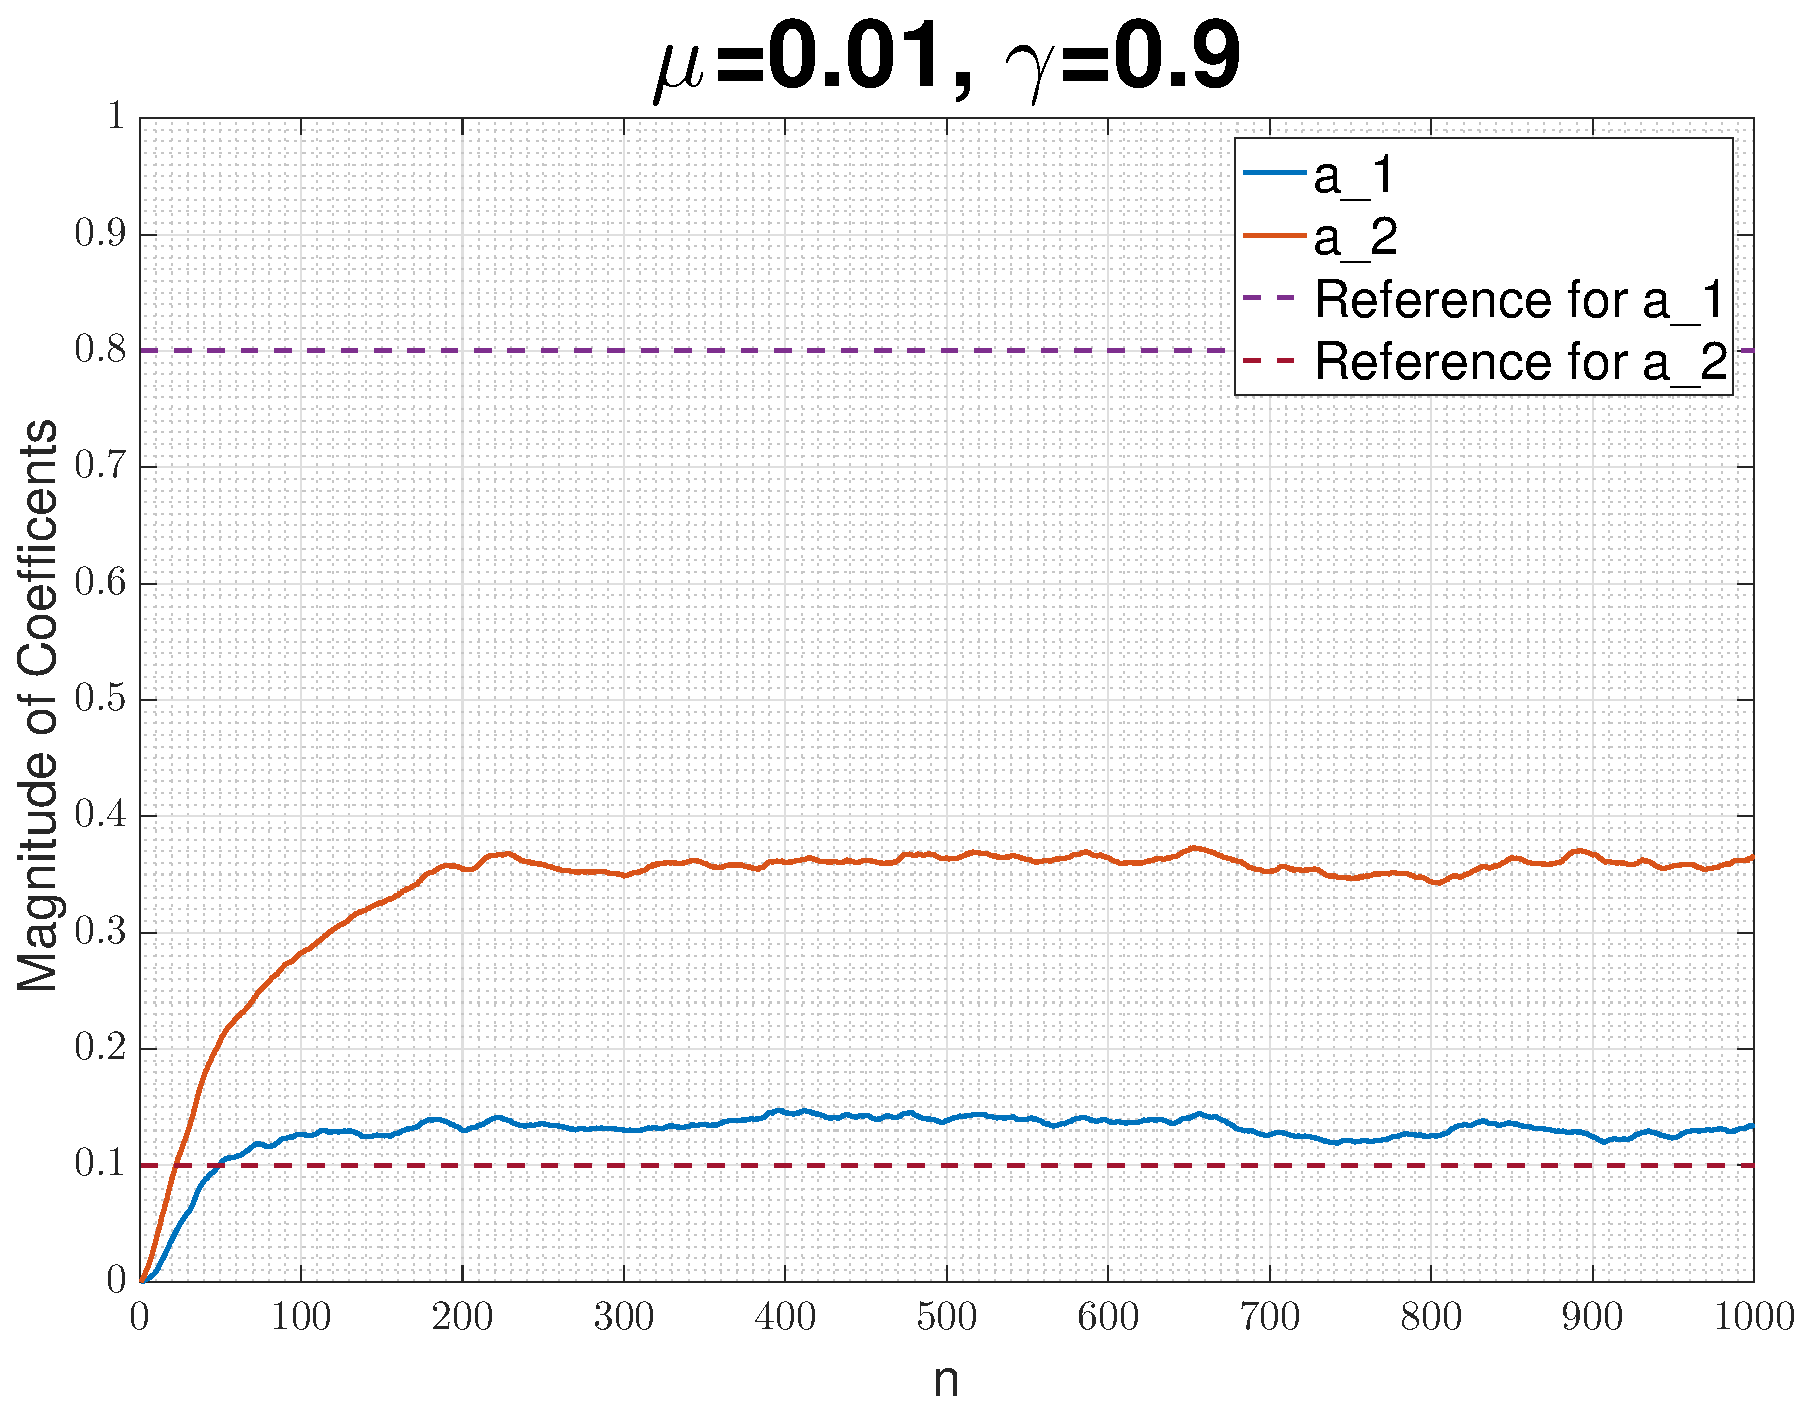
\includegraphics[width=0.32\textwidth]{part3/leaky_mu_01_gamma_09}
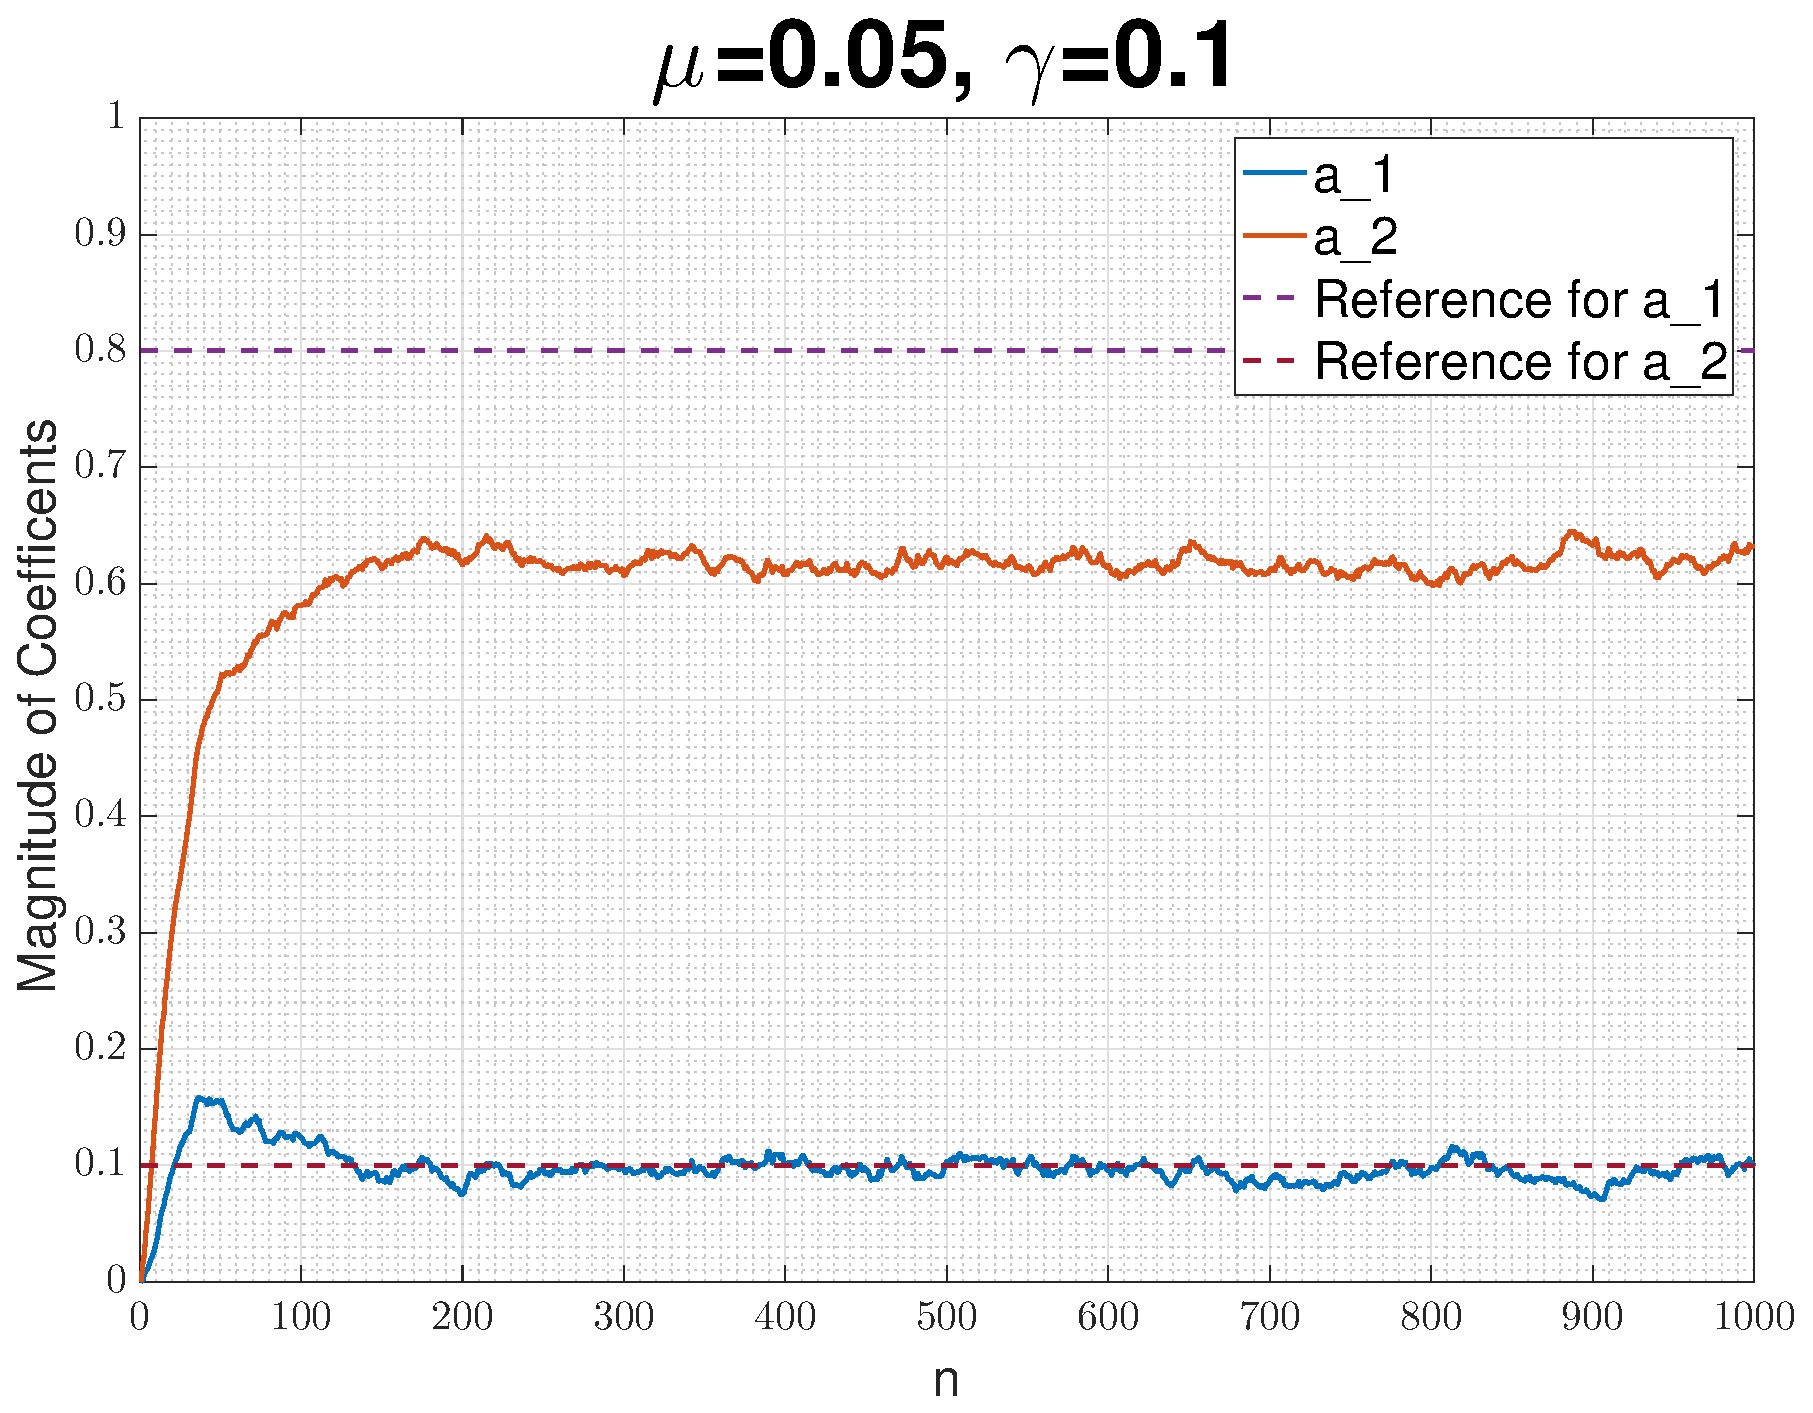
\includegraphics[width=0.32\textwidth]{part3/leaky_mu_05_gamma_01}
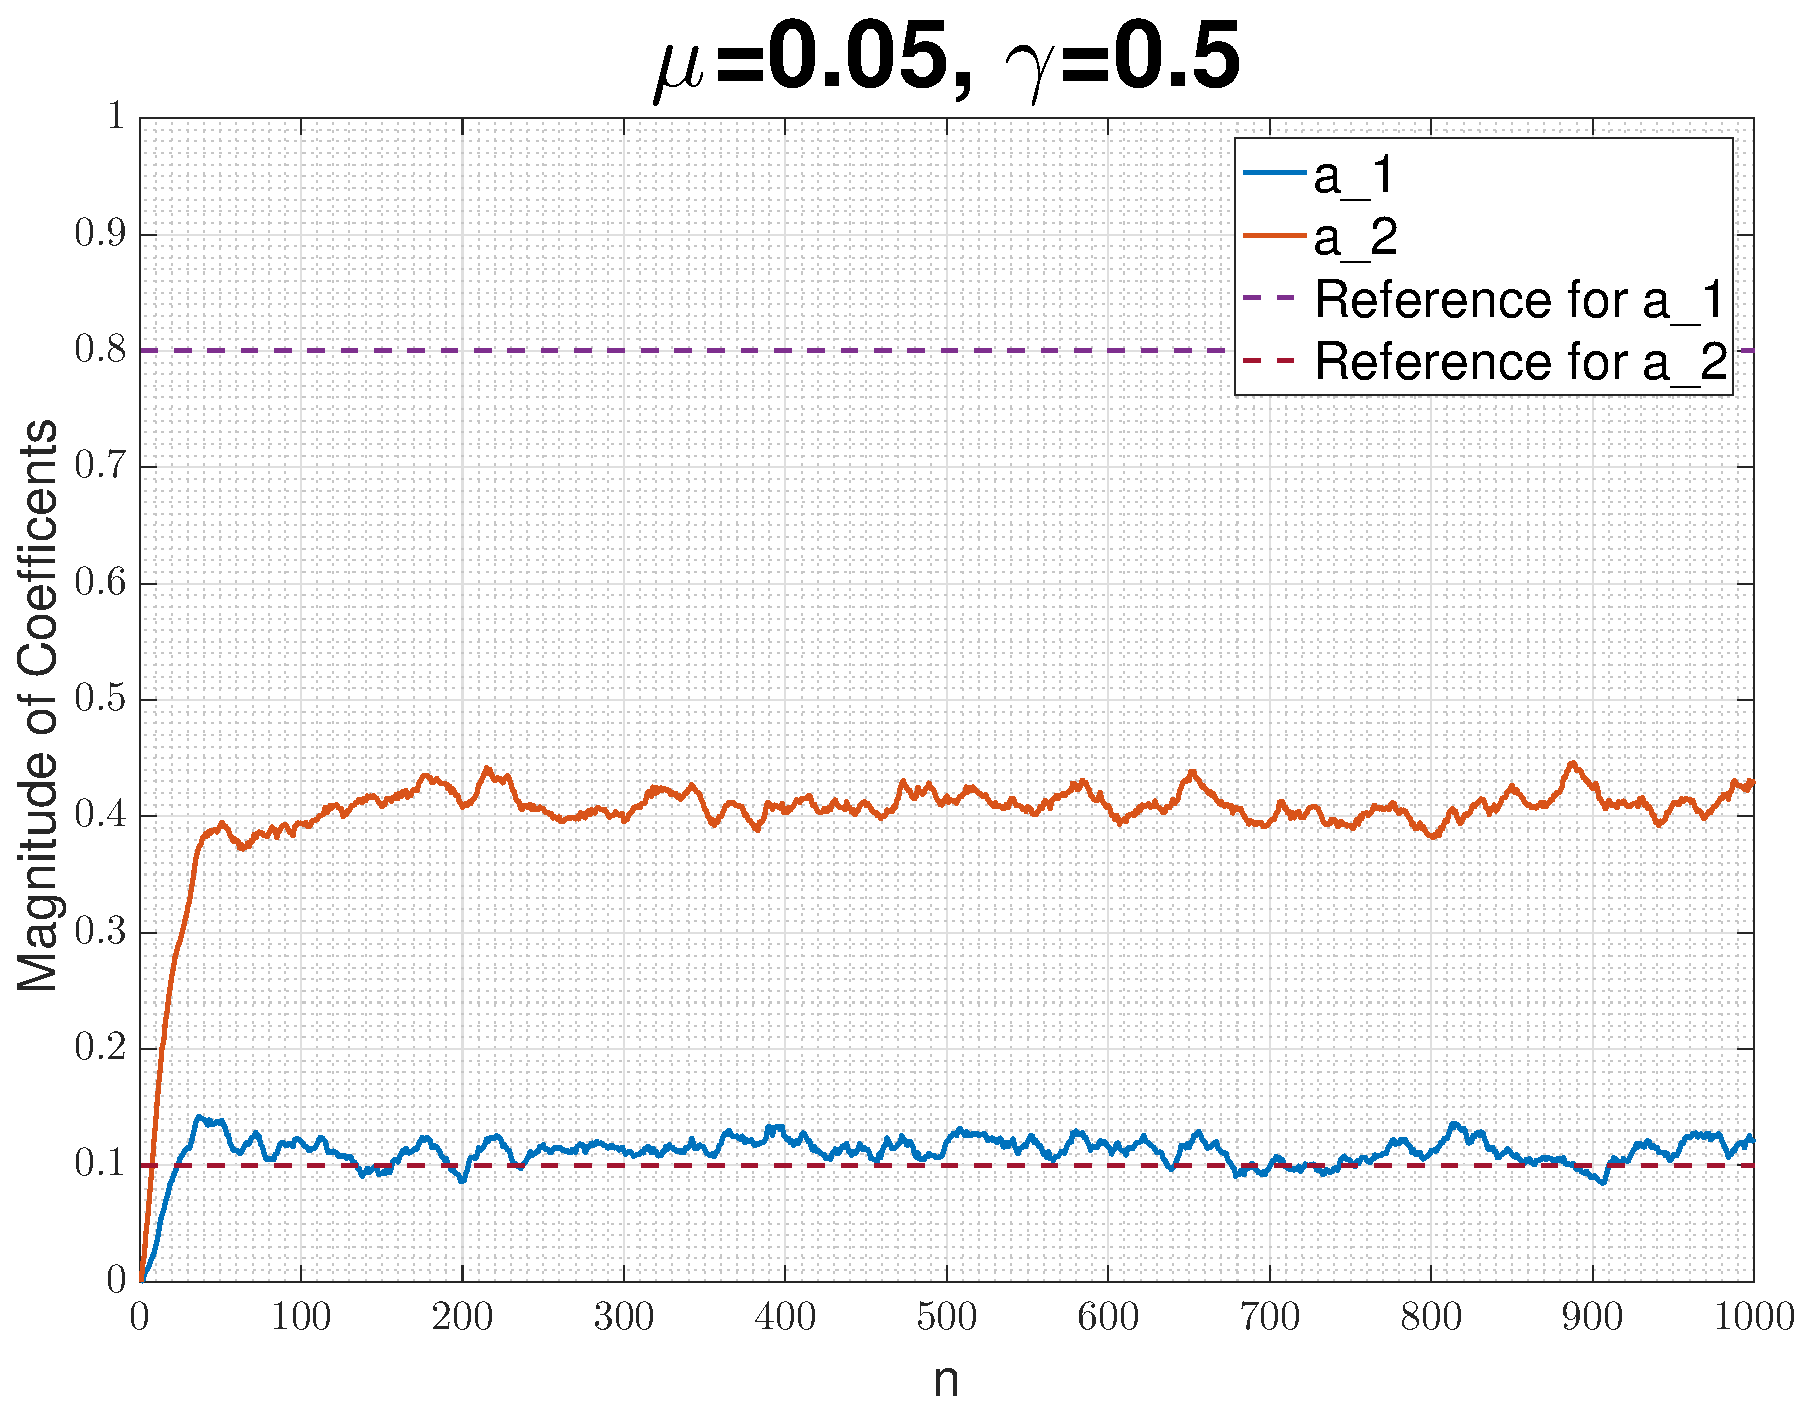
\includegraphics[width=0.32\textwidth]{part3/leaky_mu_05_gamma_05}
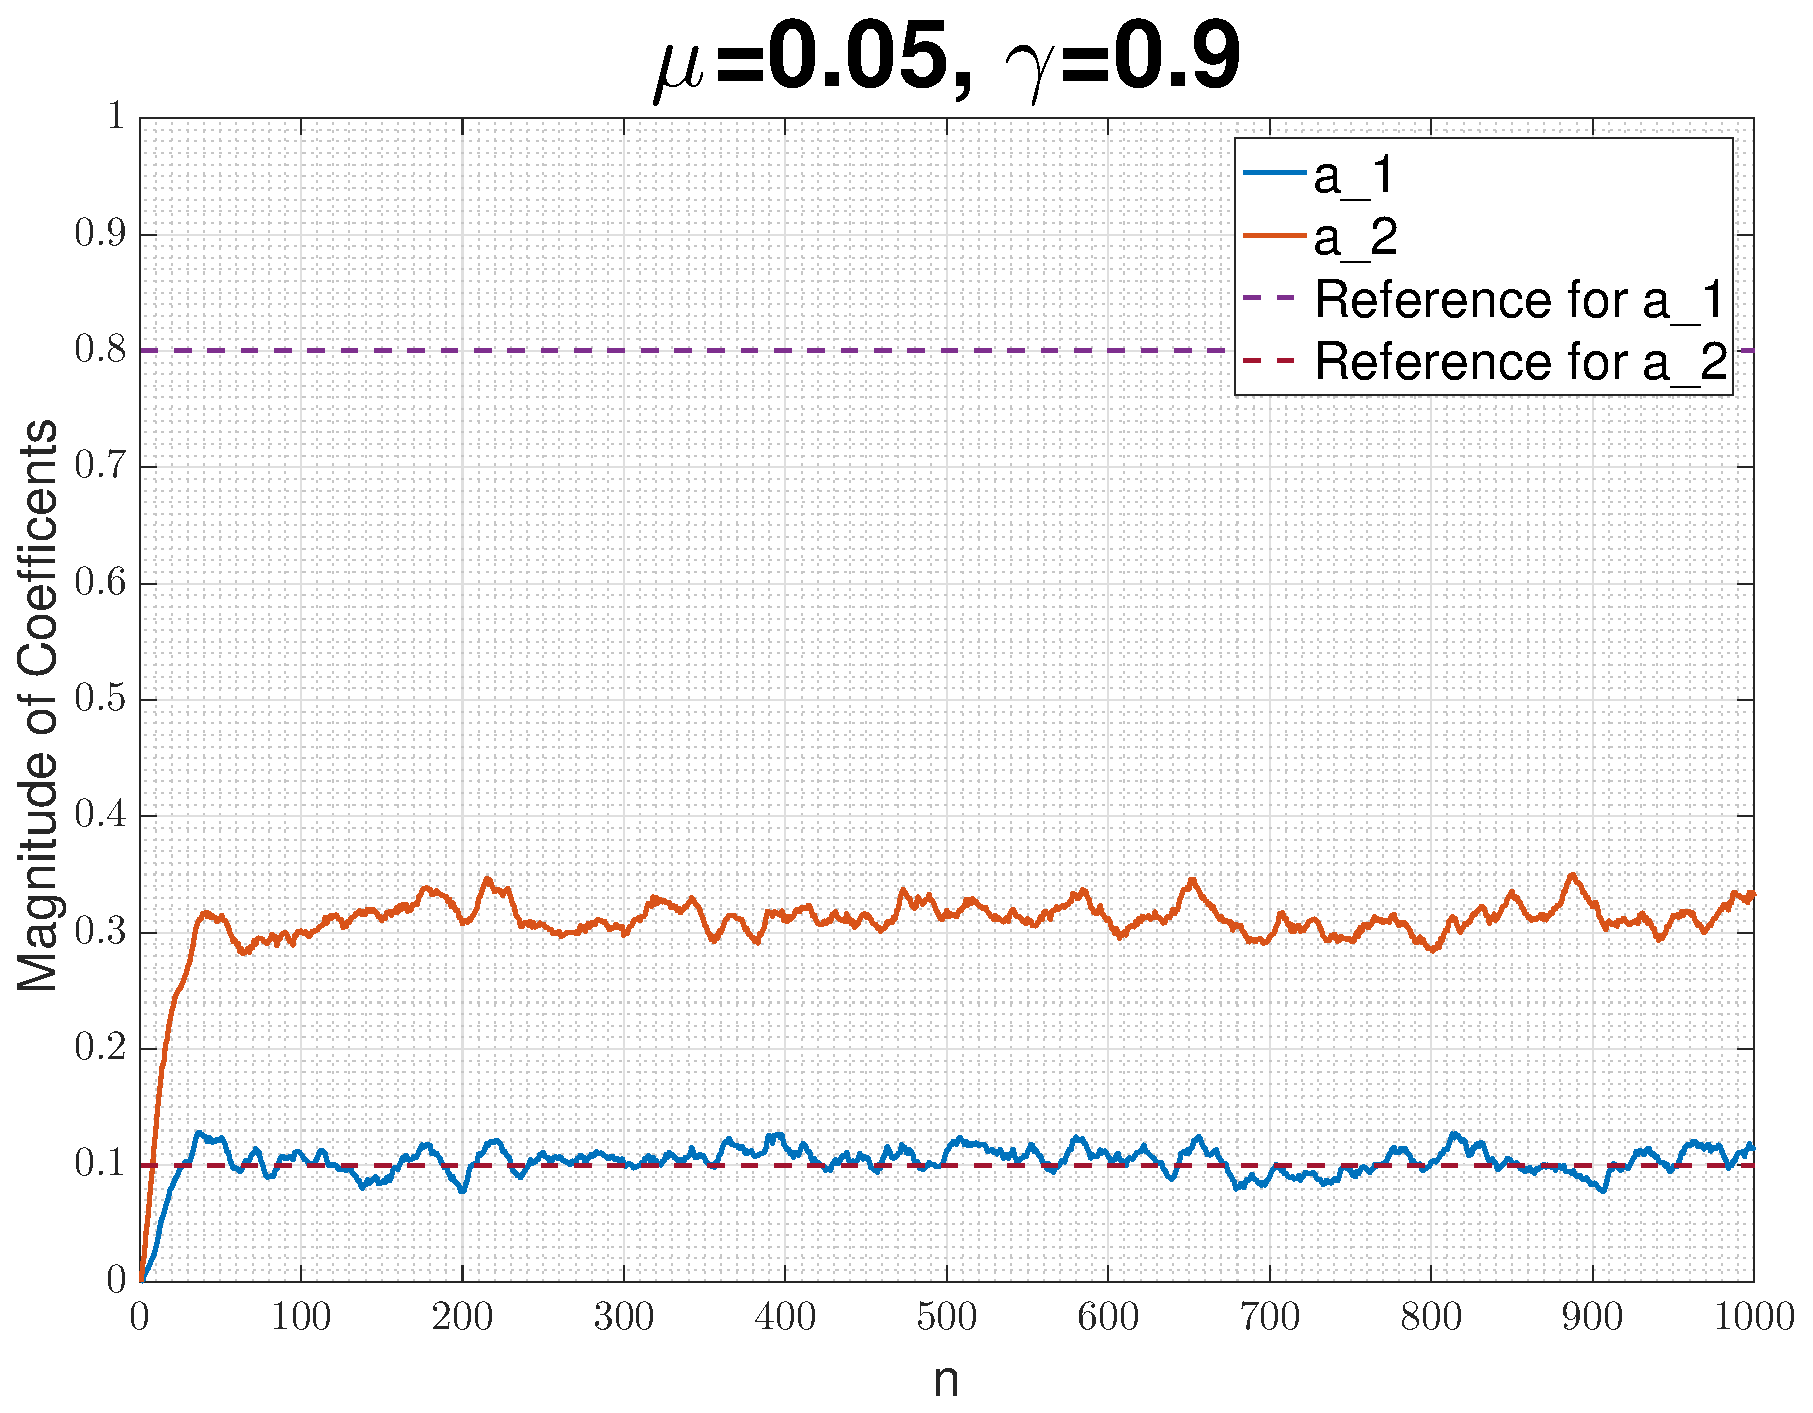
\includegraphics[width=0.32\textwidth]{part3/leaky_mu_05_gamma_09}
\caption{Effect of increasing $\gamma$ on the Steady State Values of Coefficients $a_1$ and $a_2$, for $\mu=0.01$ and $\mu=0.05$}
\end{figure}


\begin{figure}[H]
\centering{}
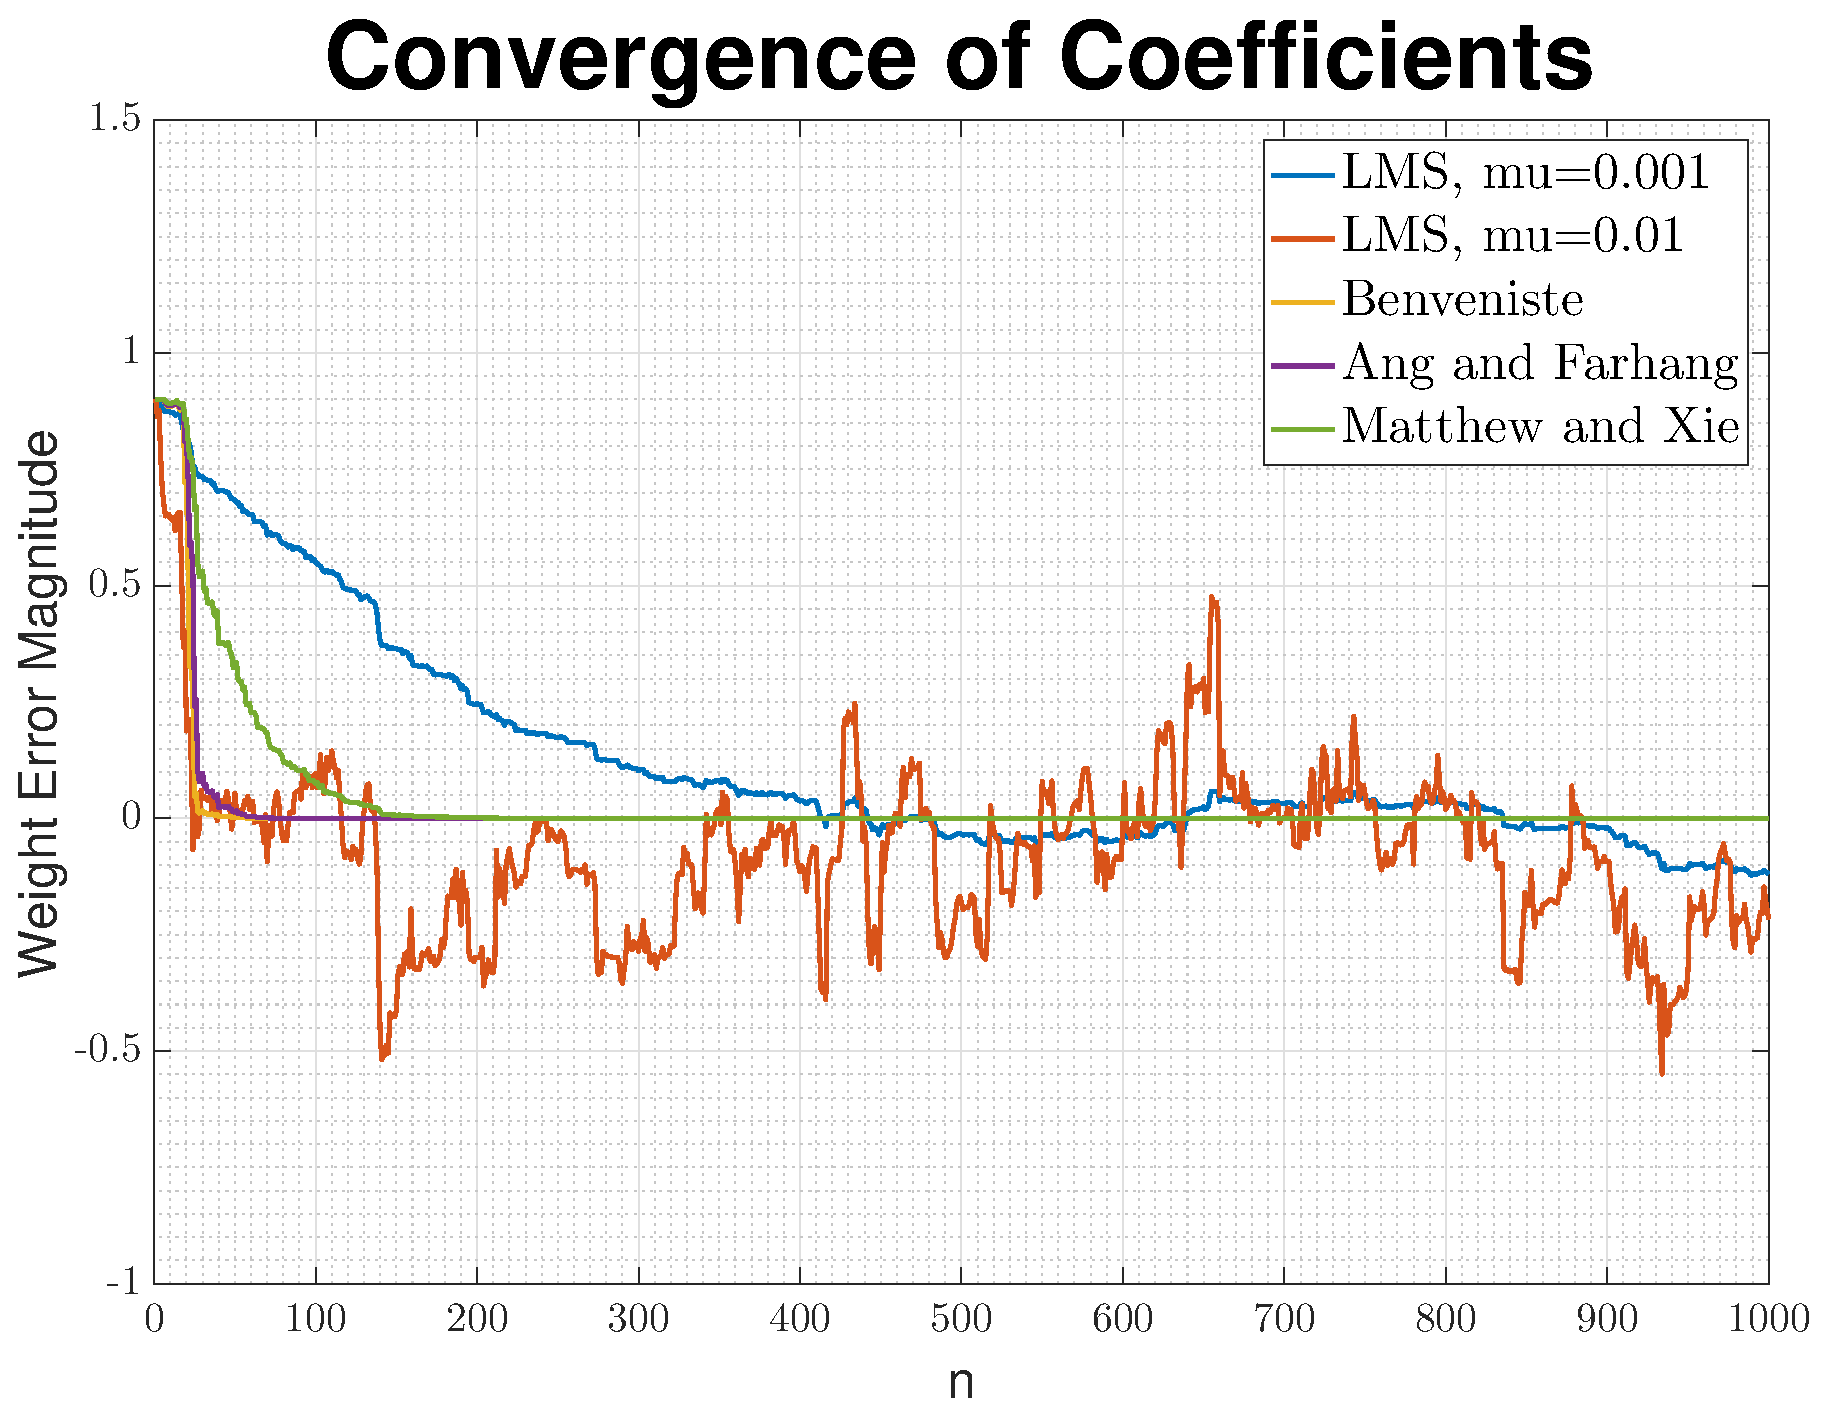
\includegraphics[width=0.32\textwidth]{part3/convergence_of_weights}
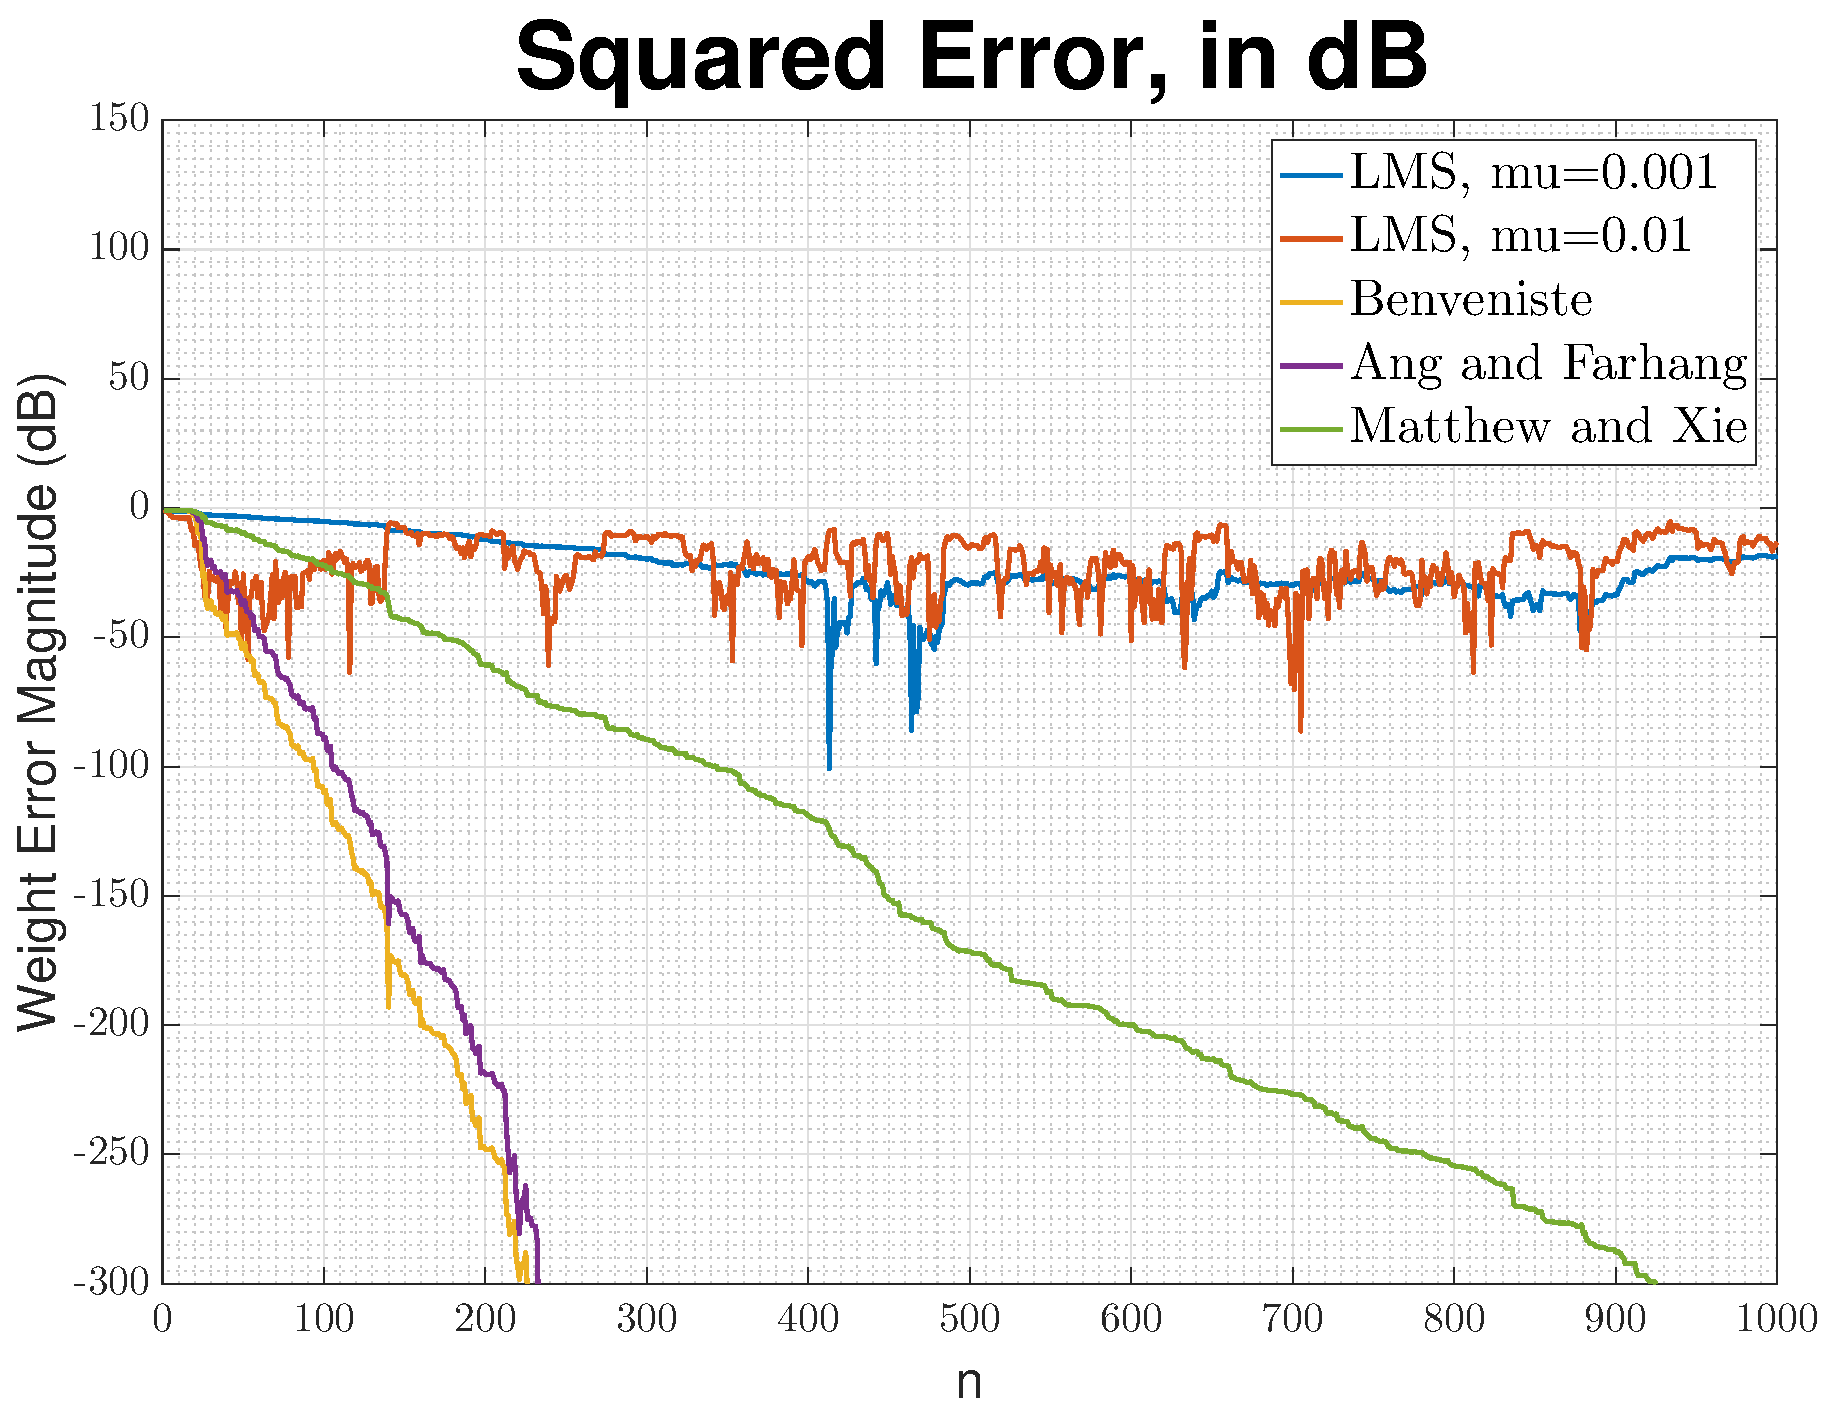
\includegraphics[width=0.32\textwidth]{part3/convergence_of_weights_db}
\caption{Comparison of Convergence Time using Adaptive Step Sizes and Standard LMS Algorithms}
\end{figure}


\begin{figure}[H]
\centering{}
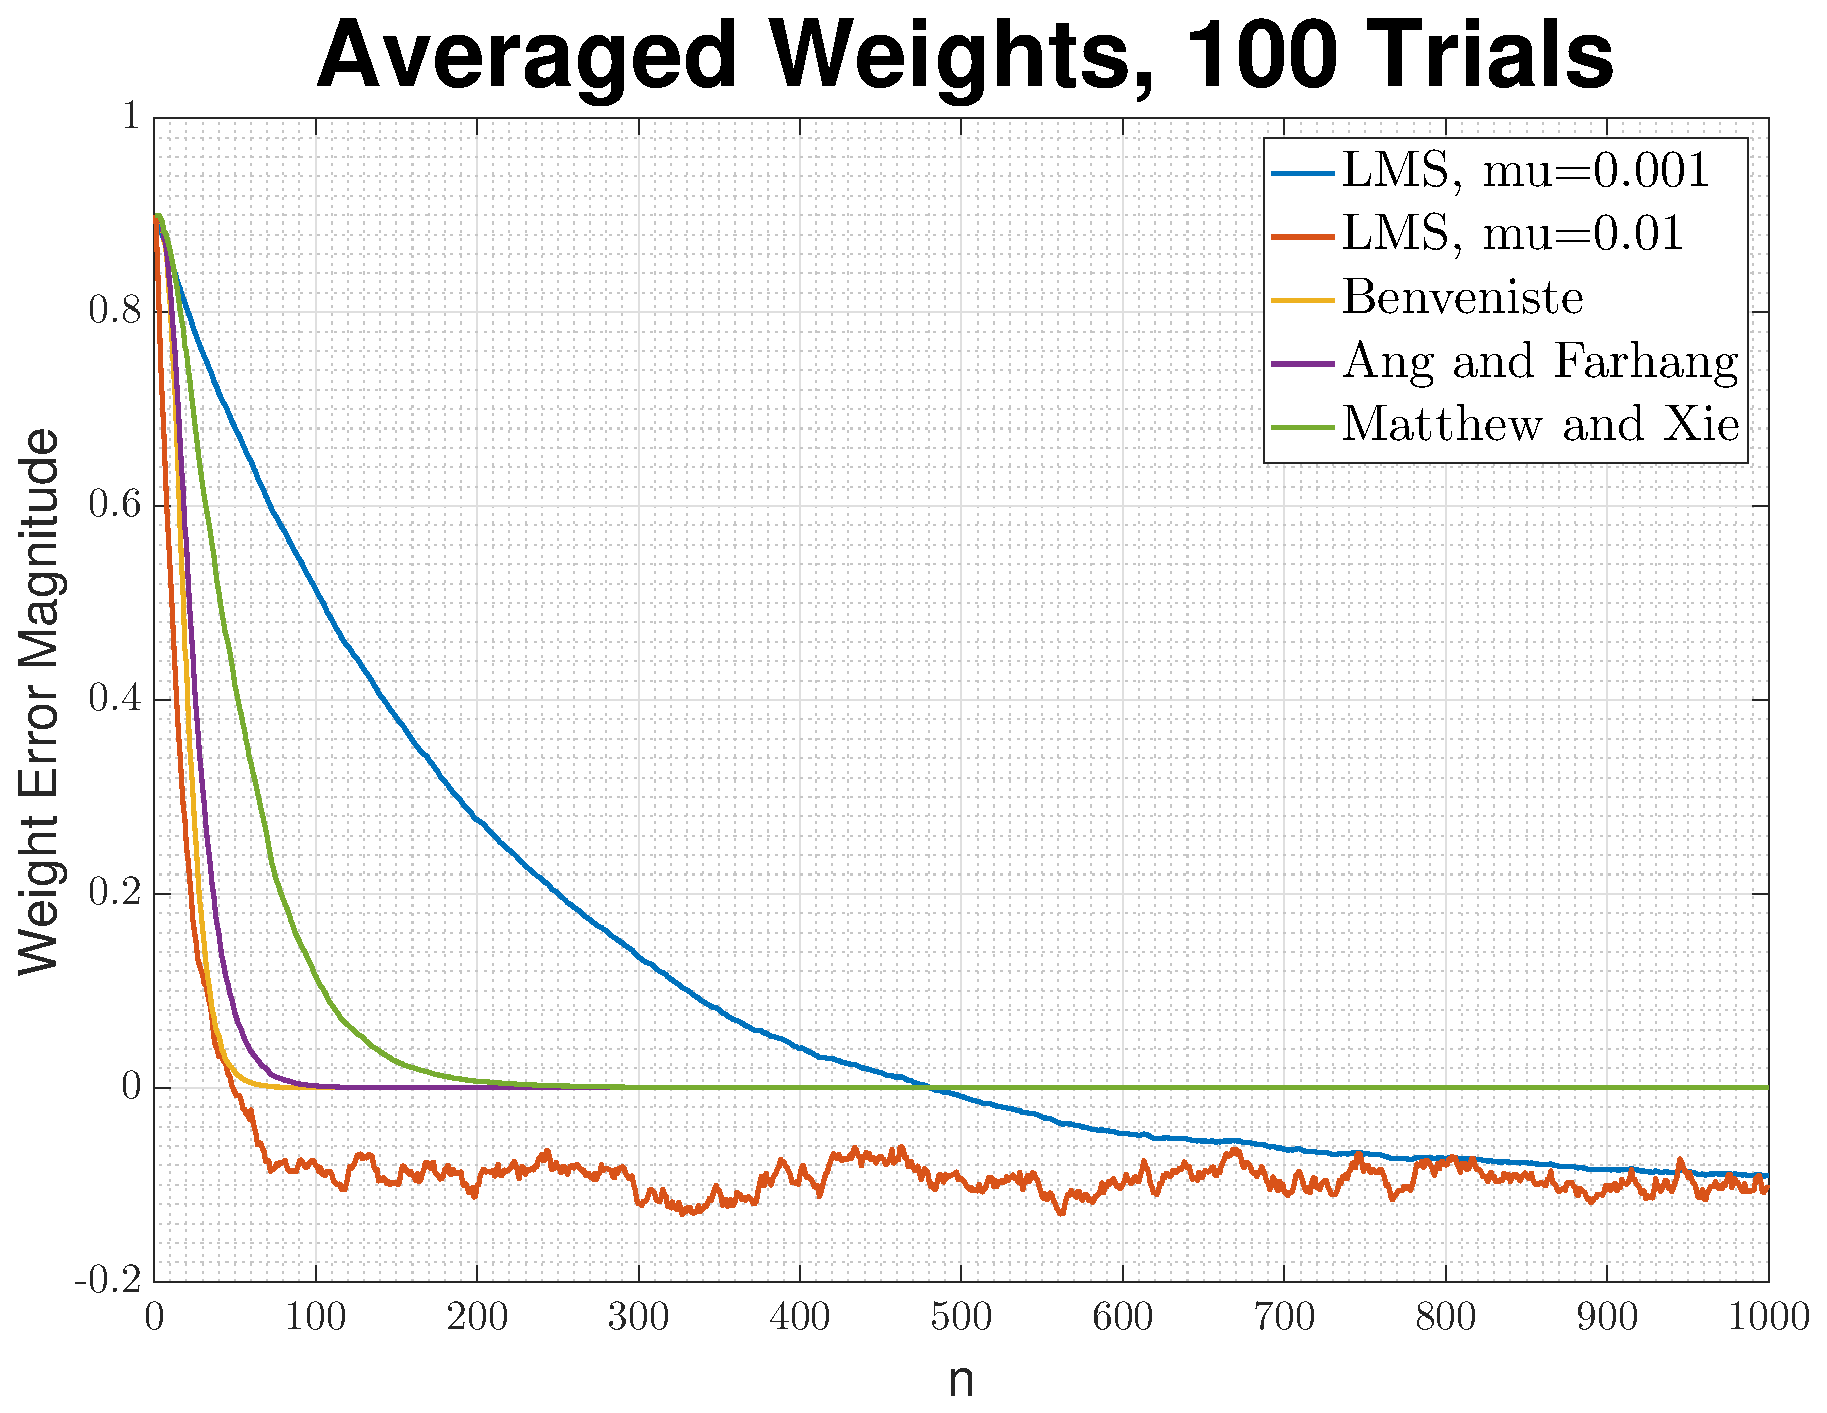
\includegraphics[width=0.32\textwidth]{part3/convergence_of_weights_averaged}
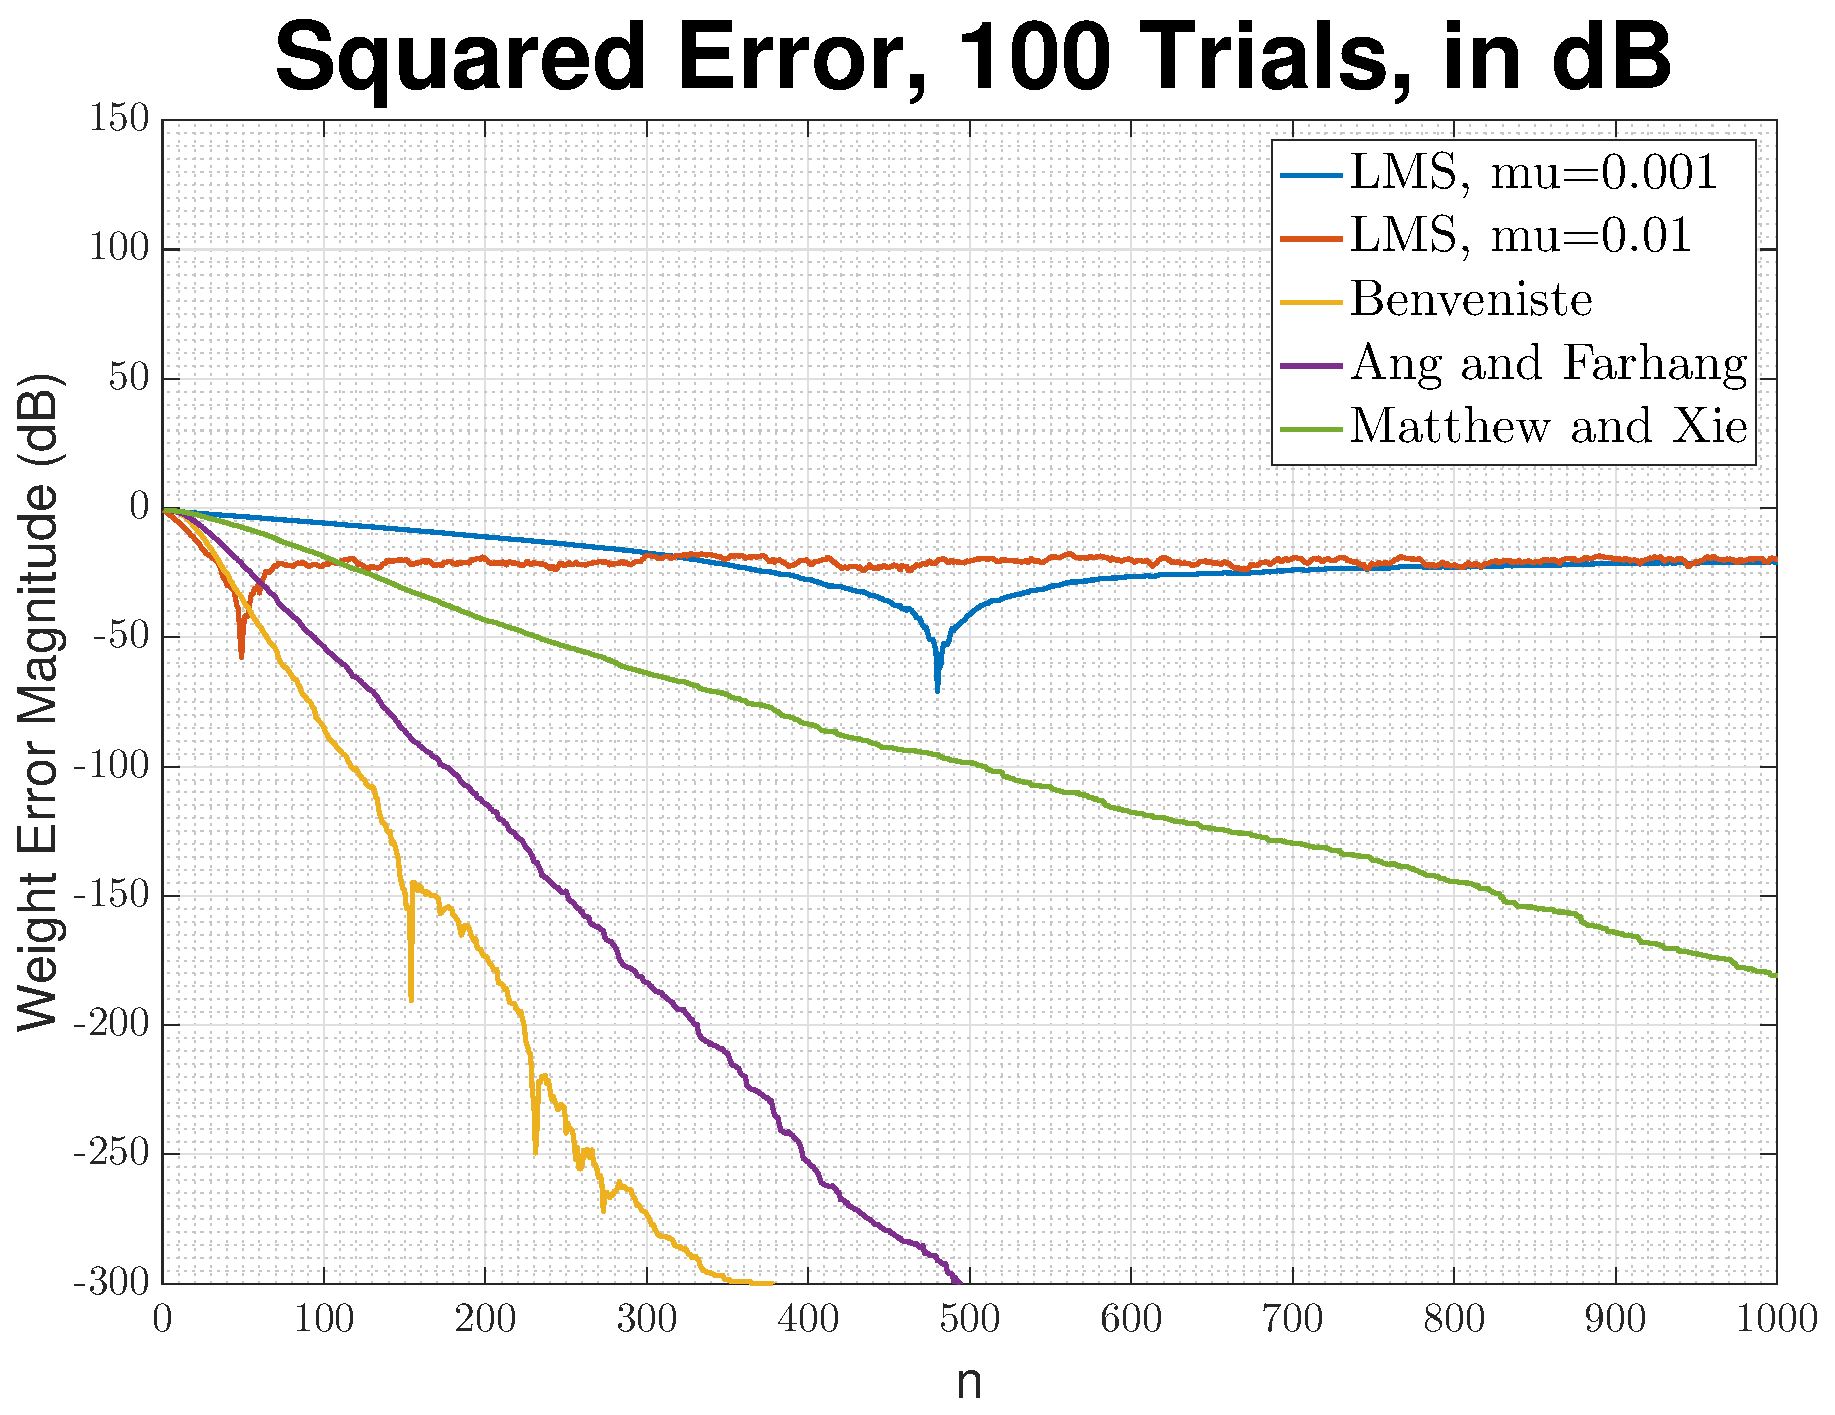
\includegraphics[width=0.32\textwidth]{part3/convergence_of_weights_averaged_db}
\caption{Studying Convergence Time by Averaging Weights over 100 Random Realisations}
\end{figure}


\begin{figure}[H]
\centering{}
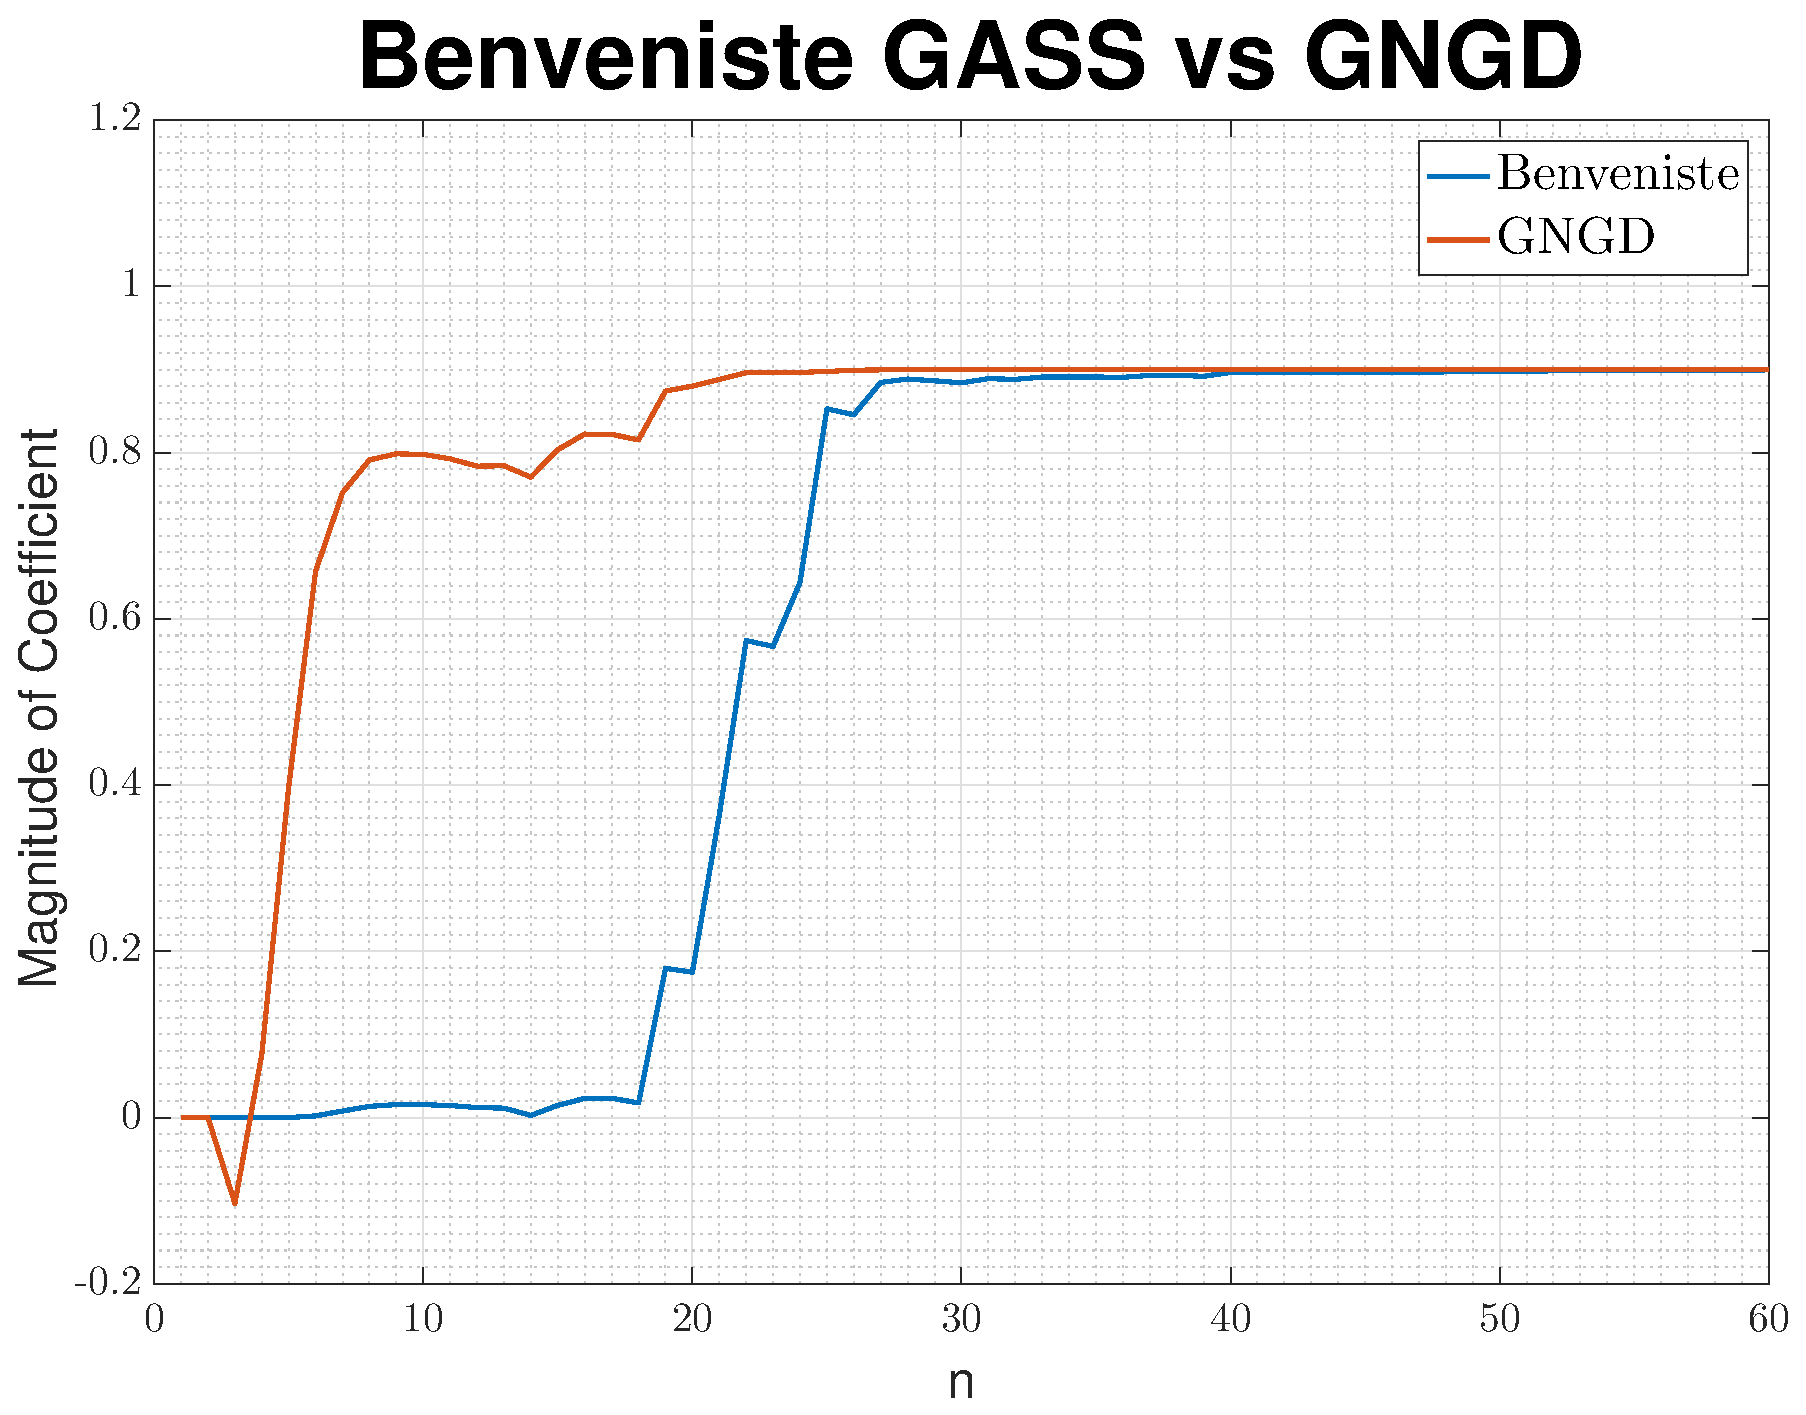
\includegraphics[width=0.32\textwidth]{part3/compare_benveniste_gngd}
\caption{Comparing Convergence Speed of GNGD and Benveniste's GASS Algorithms}
\end{figure}


\begin{figure}[H]
\centering{}
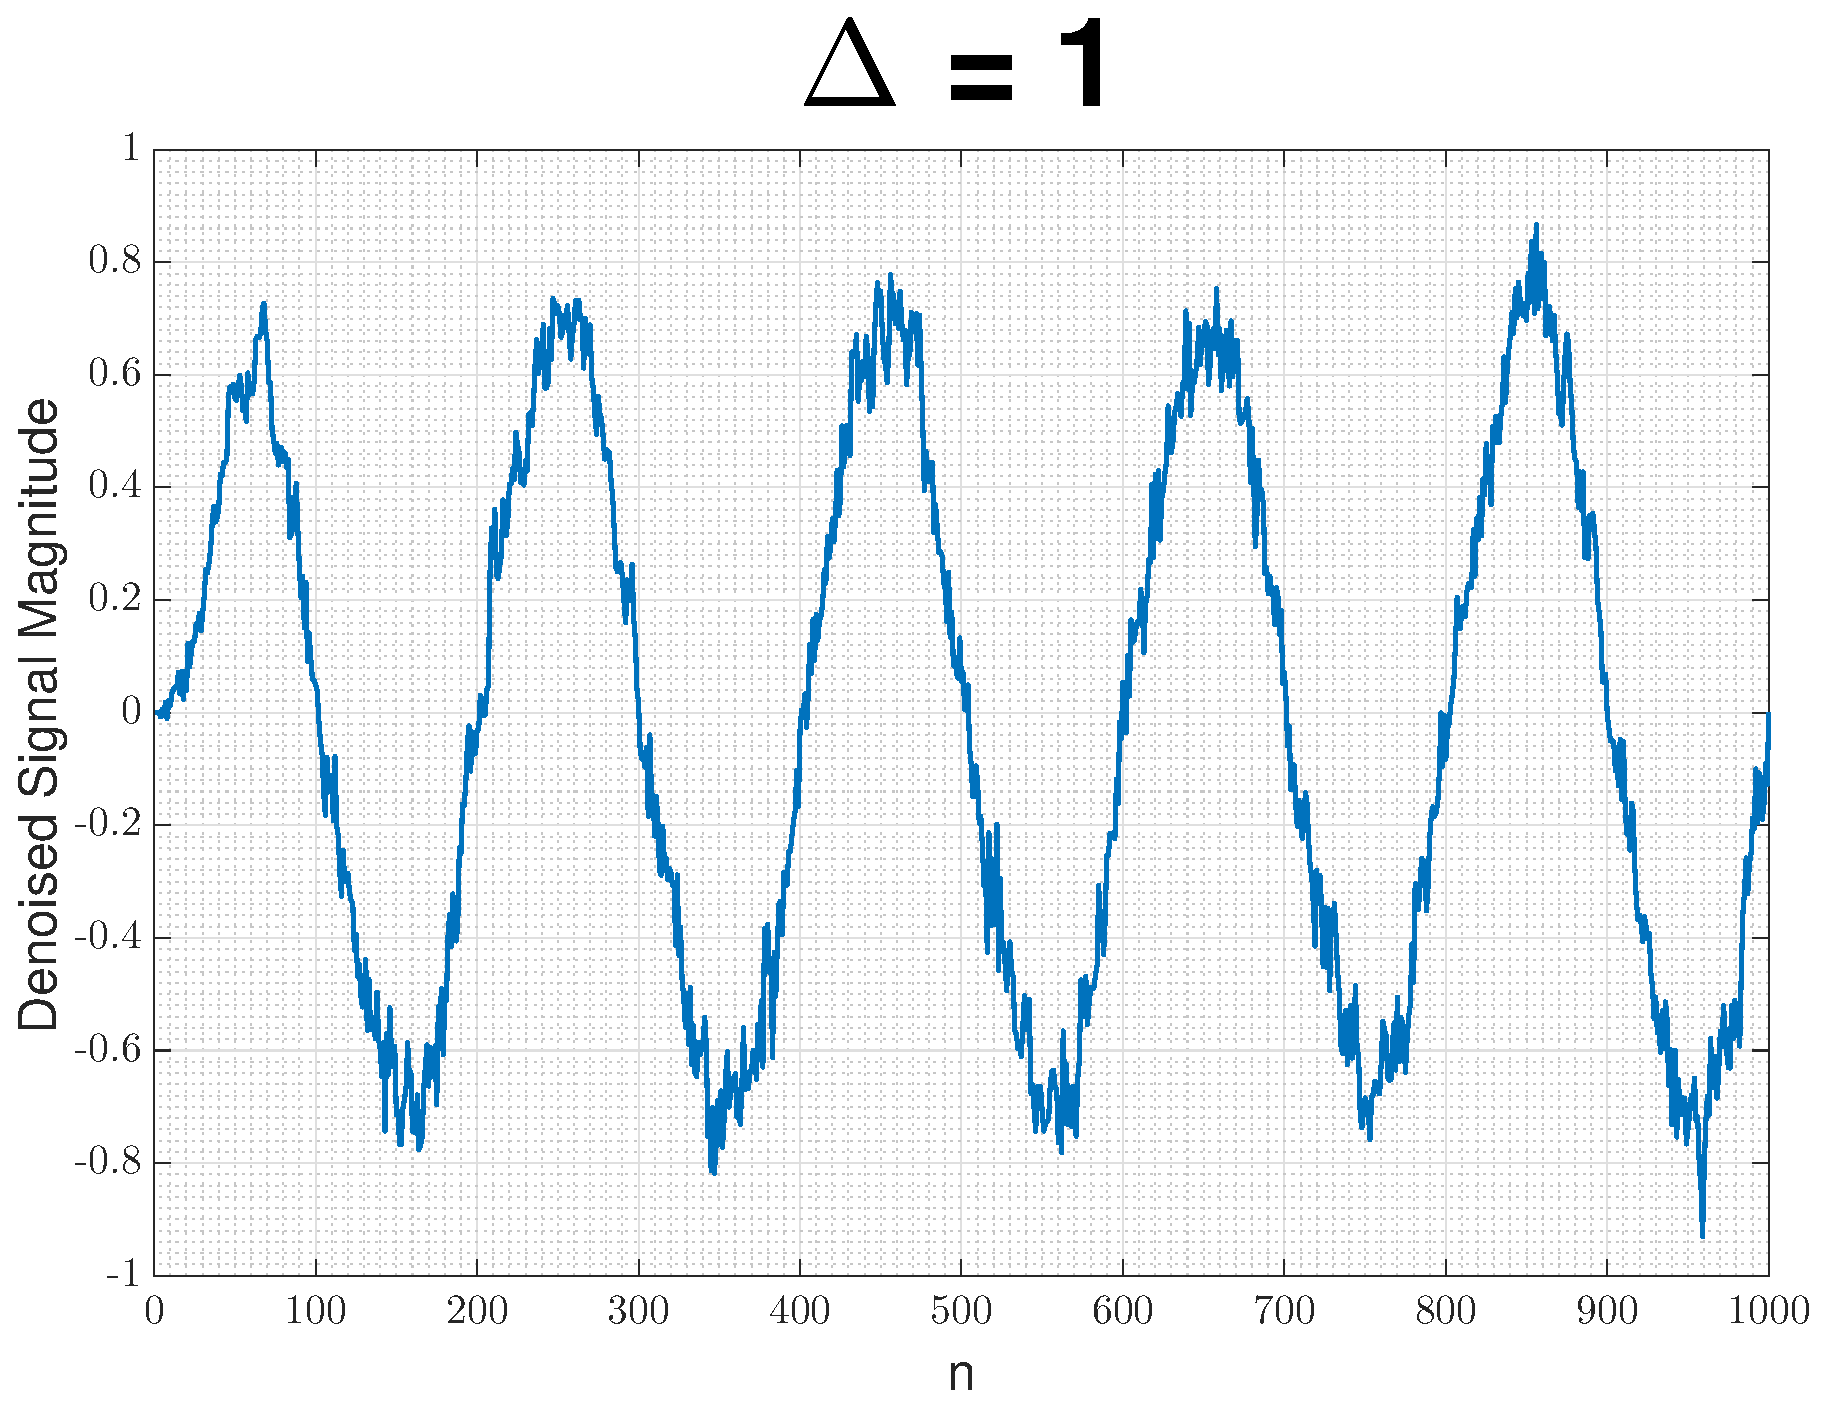
\includegraphics[width=0.24\textwidth]{part3/delay_1}
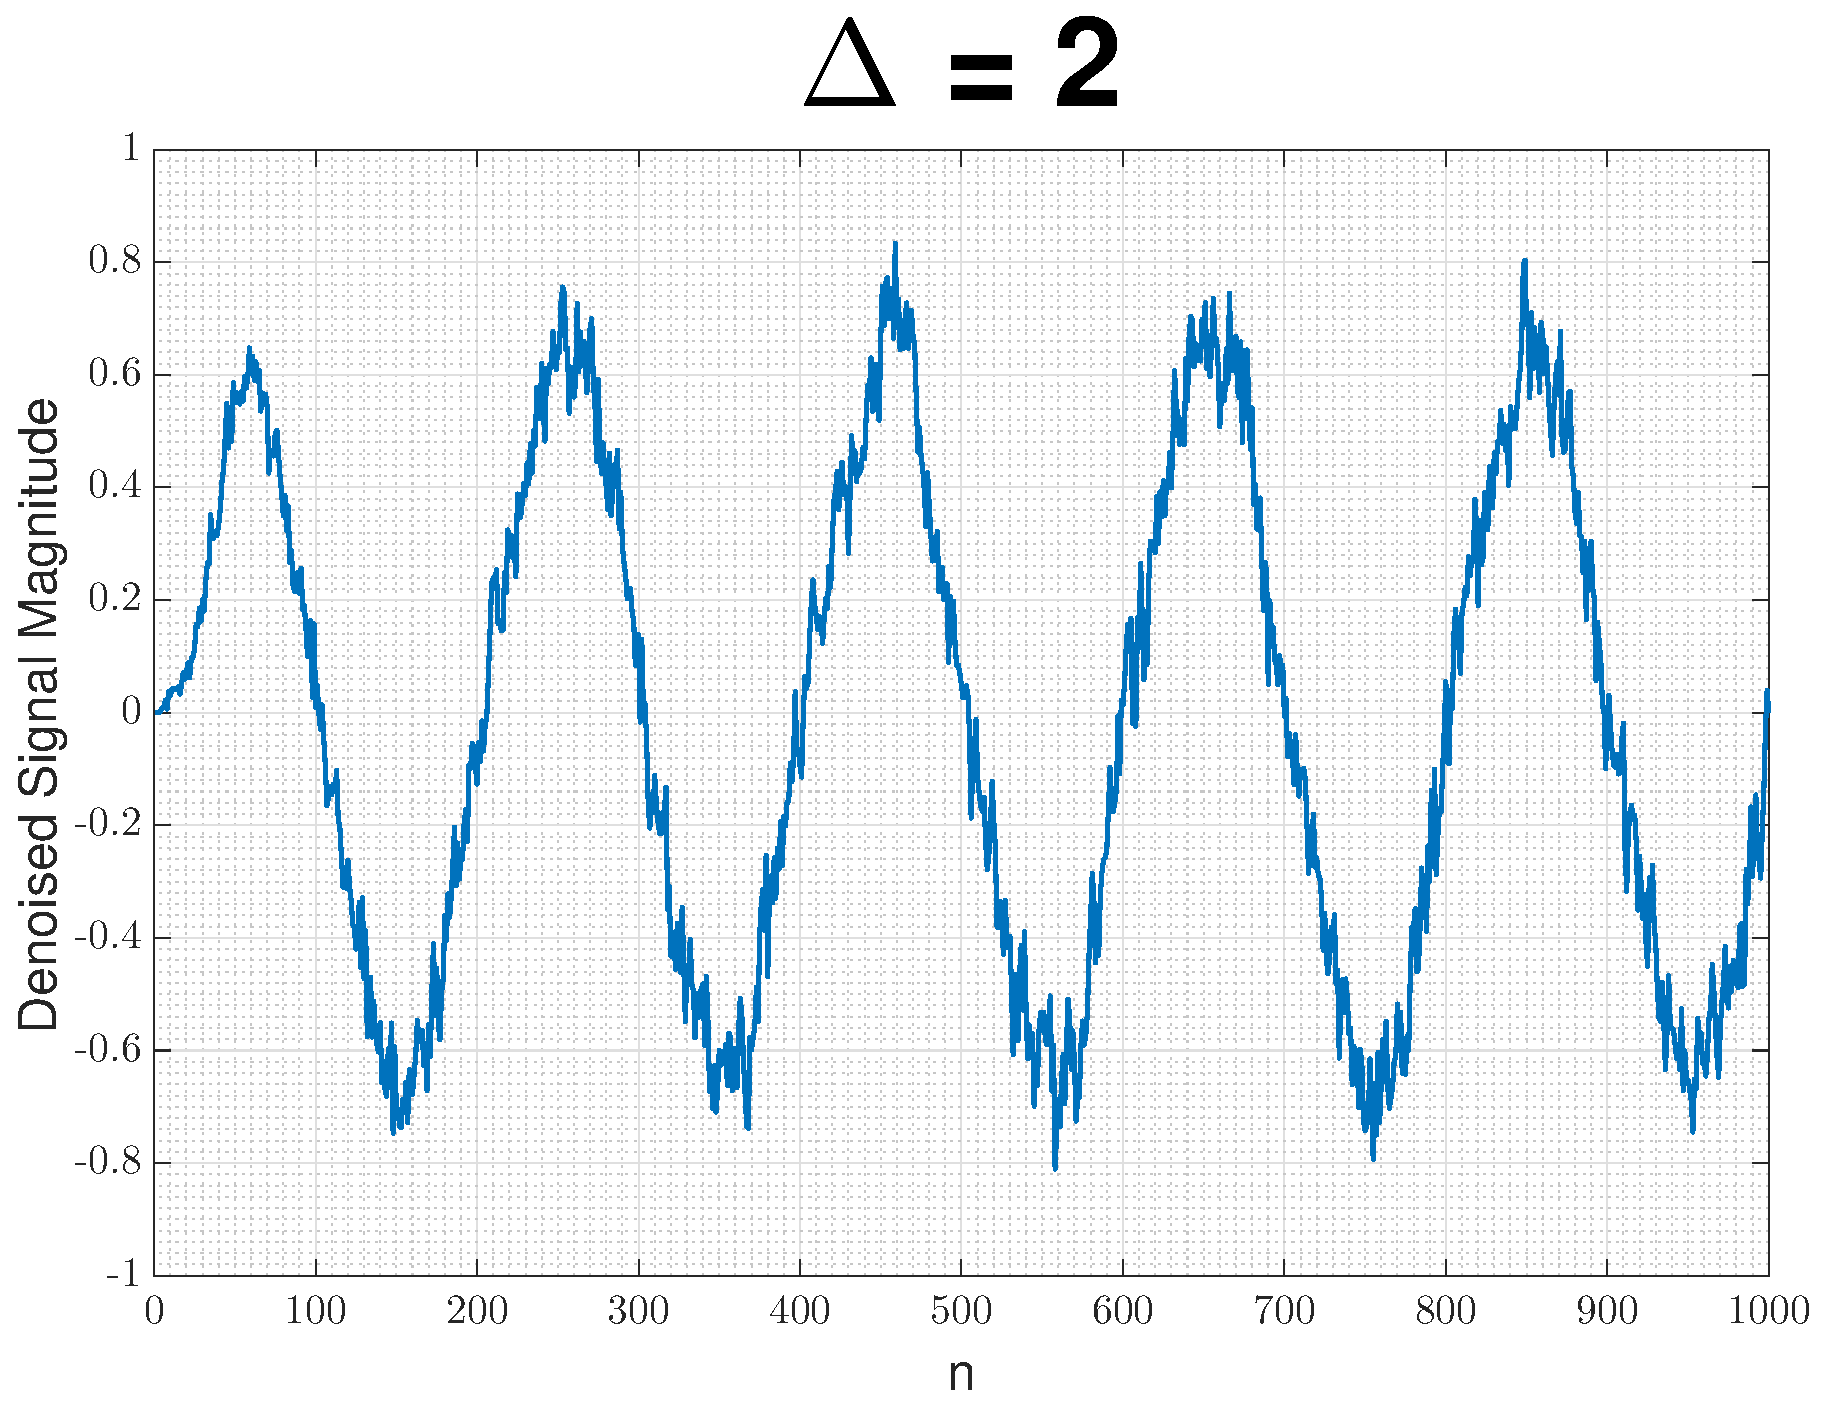
\includegraphics[width=0.24\textwidth]{part3/delay_2}
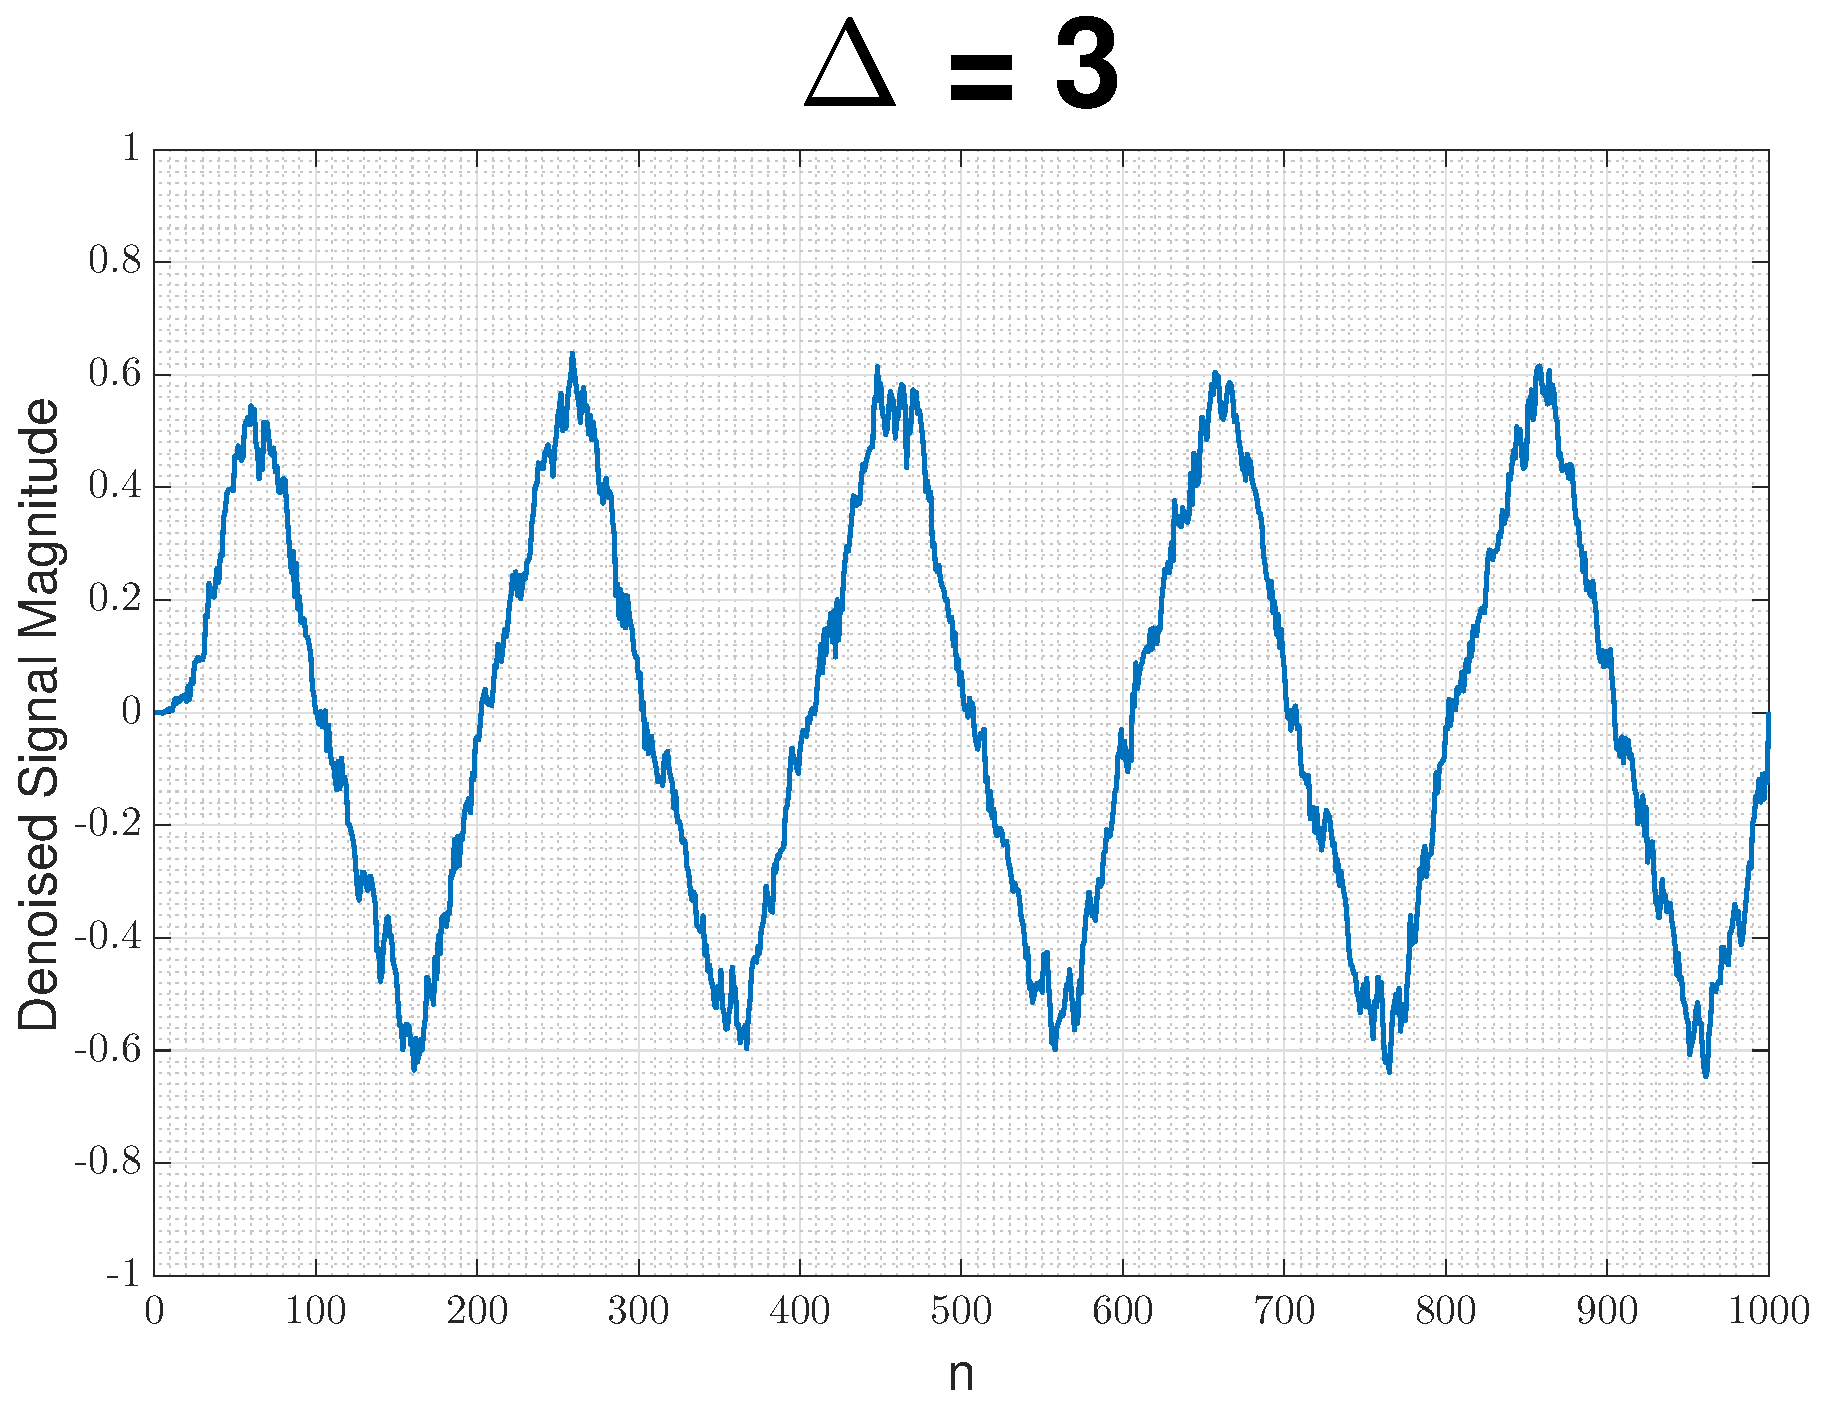
\includegraphics[width=0.24\textwidth]{part3/delay_3}
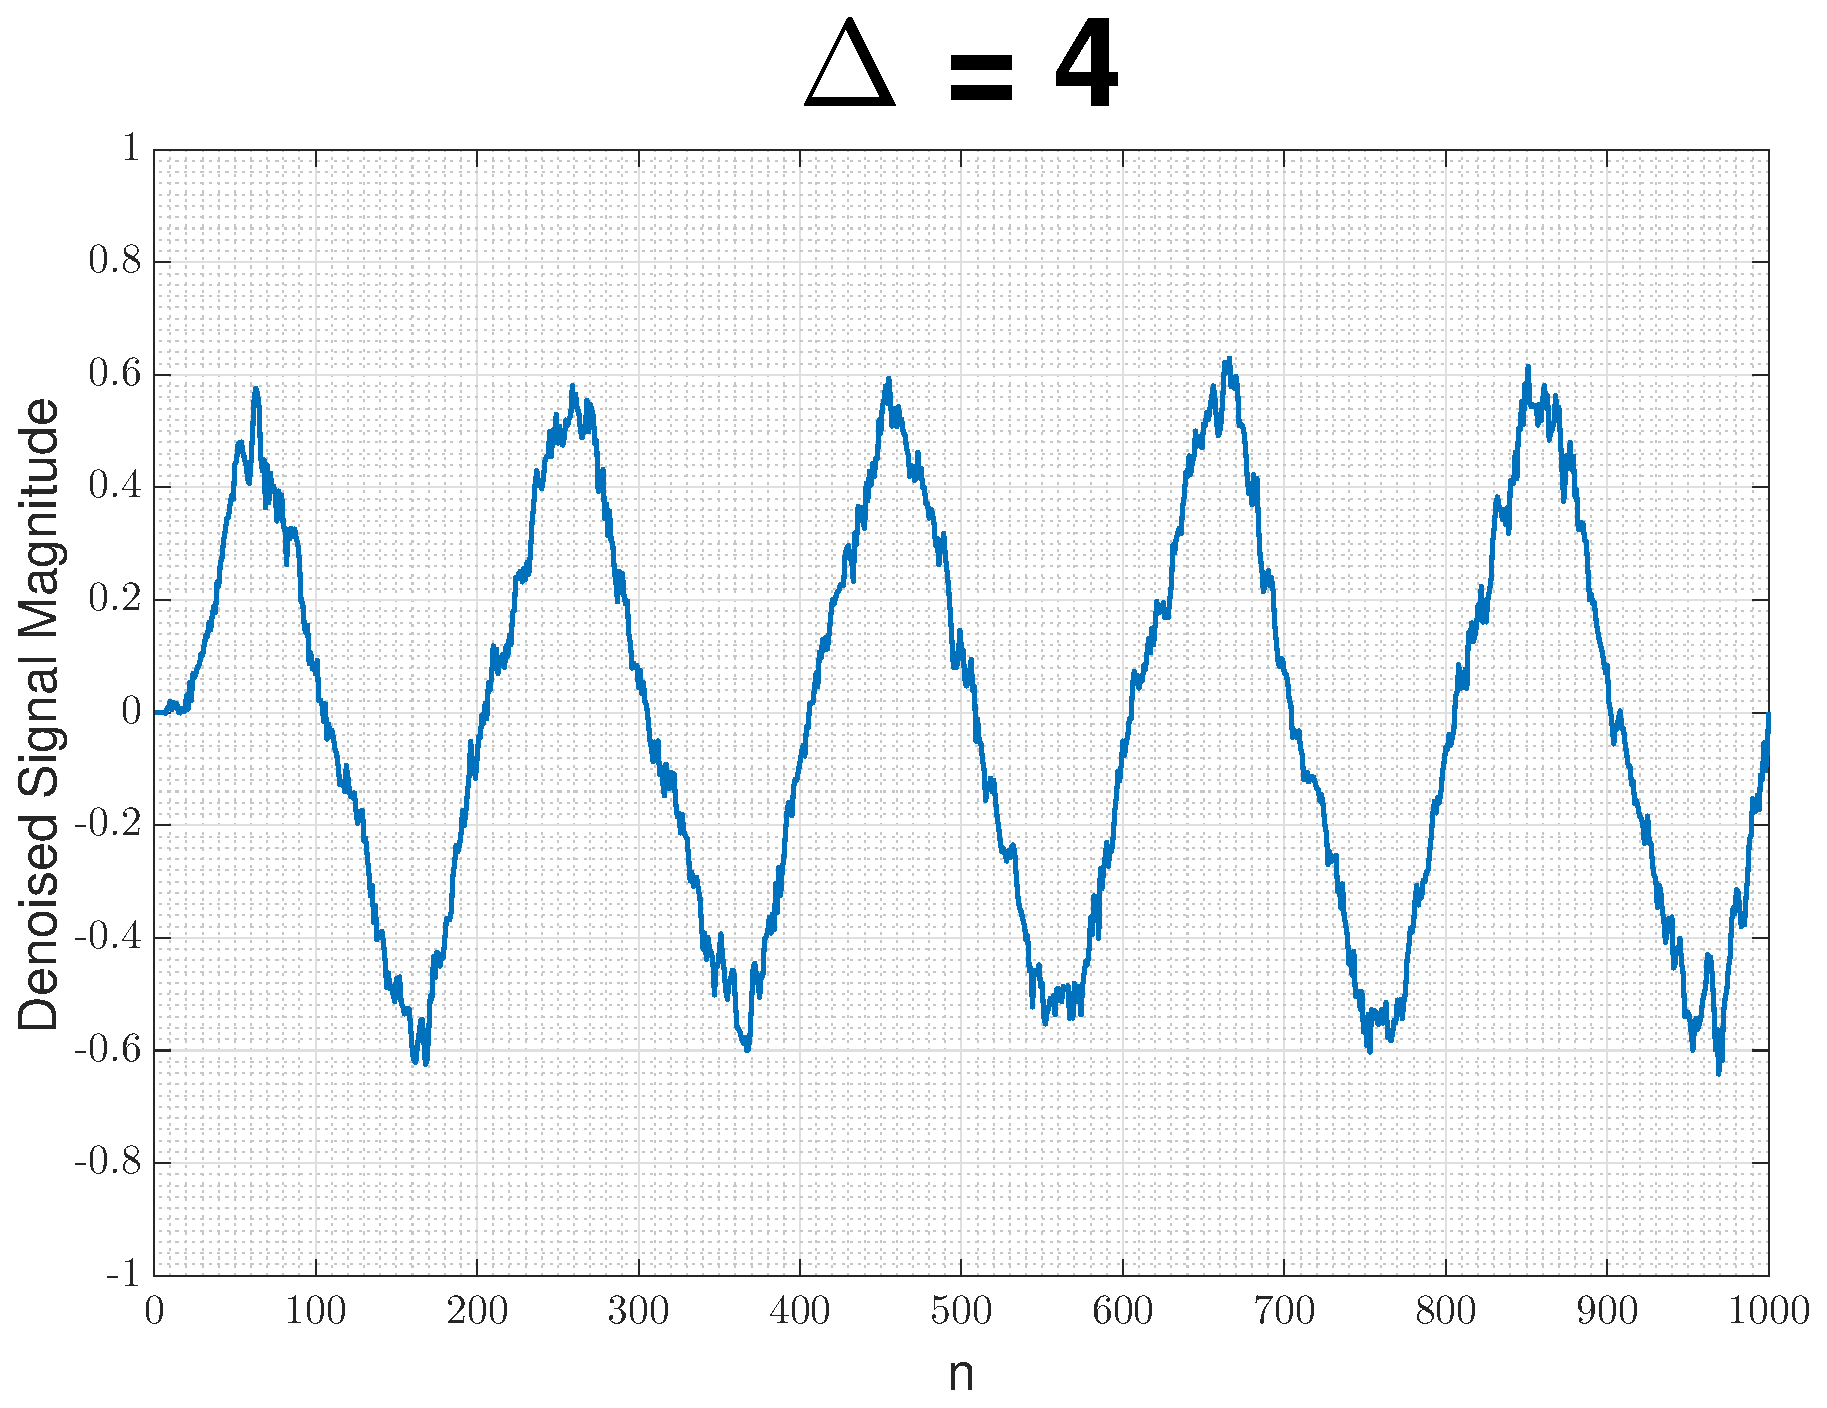
\includegraphics[width=0.24\textwidth]{part3/delay_4}
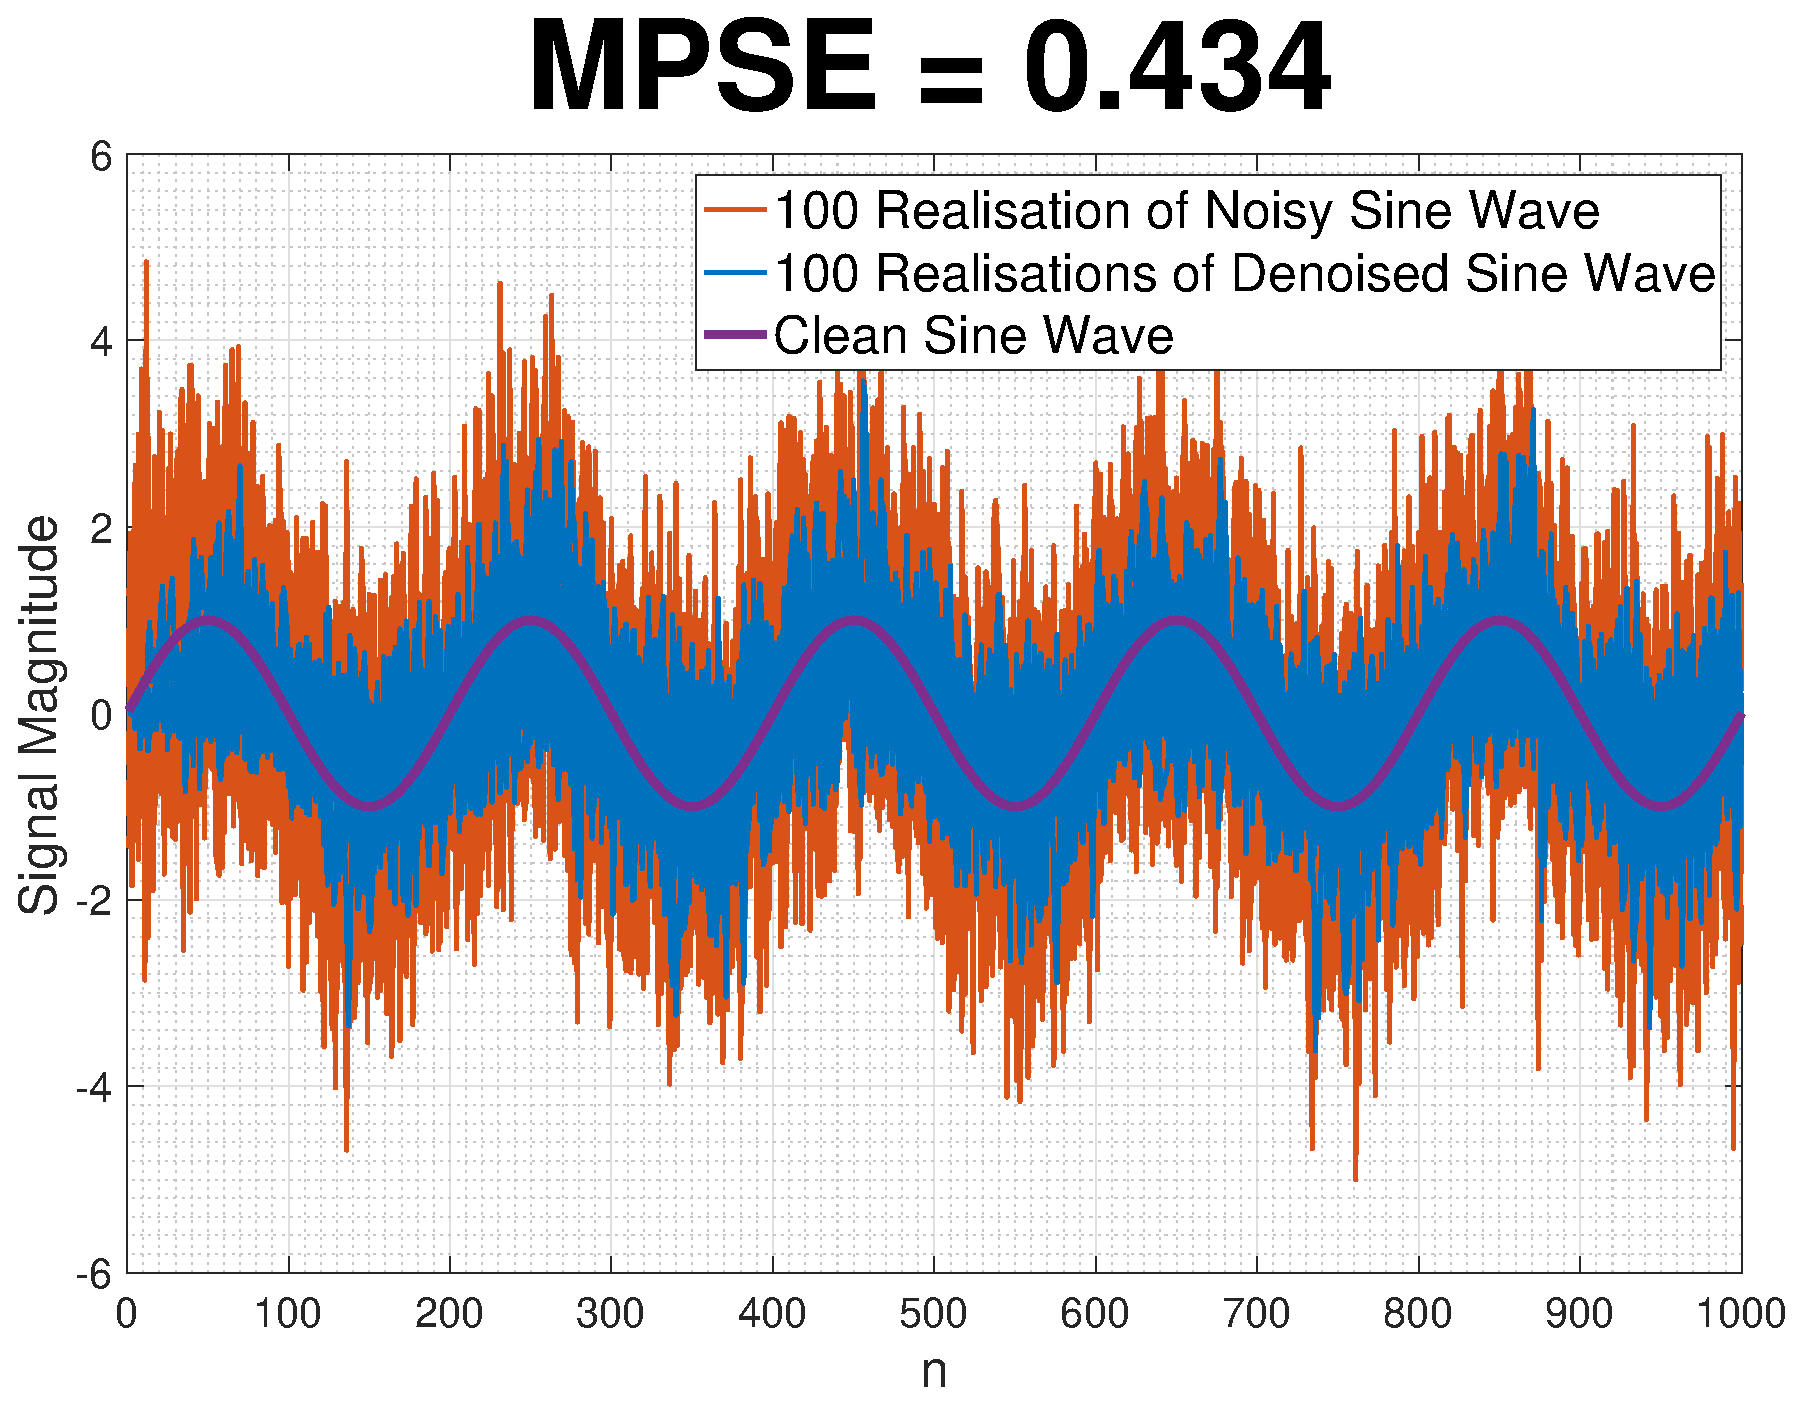
\includegraphics[width=0.24\textwidth]{part3/mpse_delay_1}
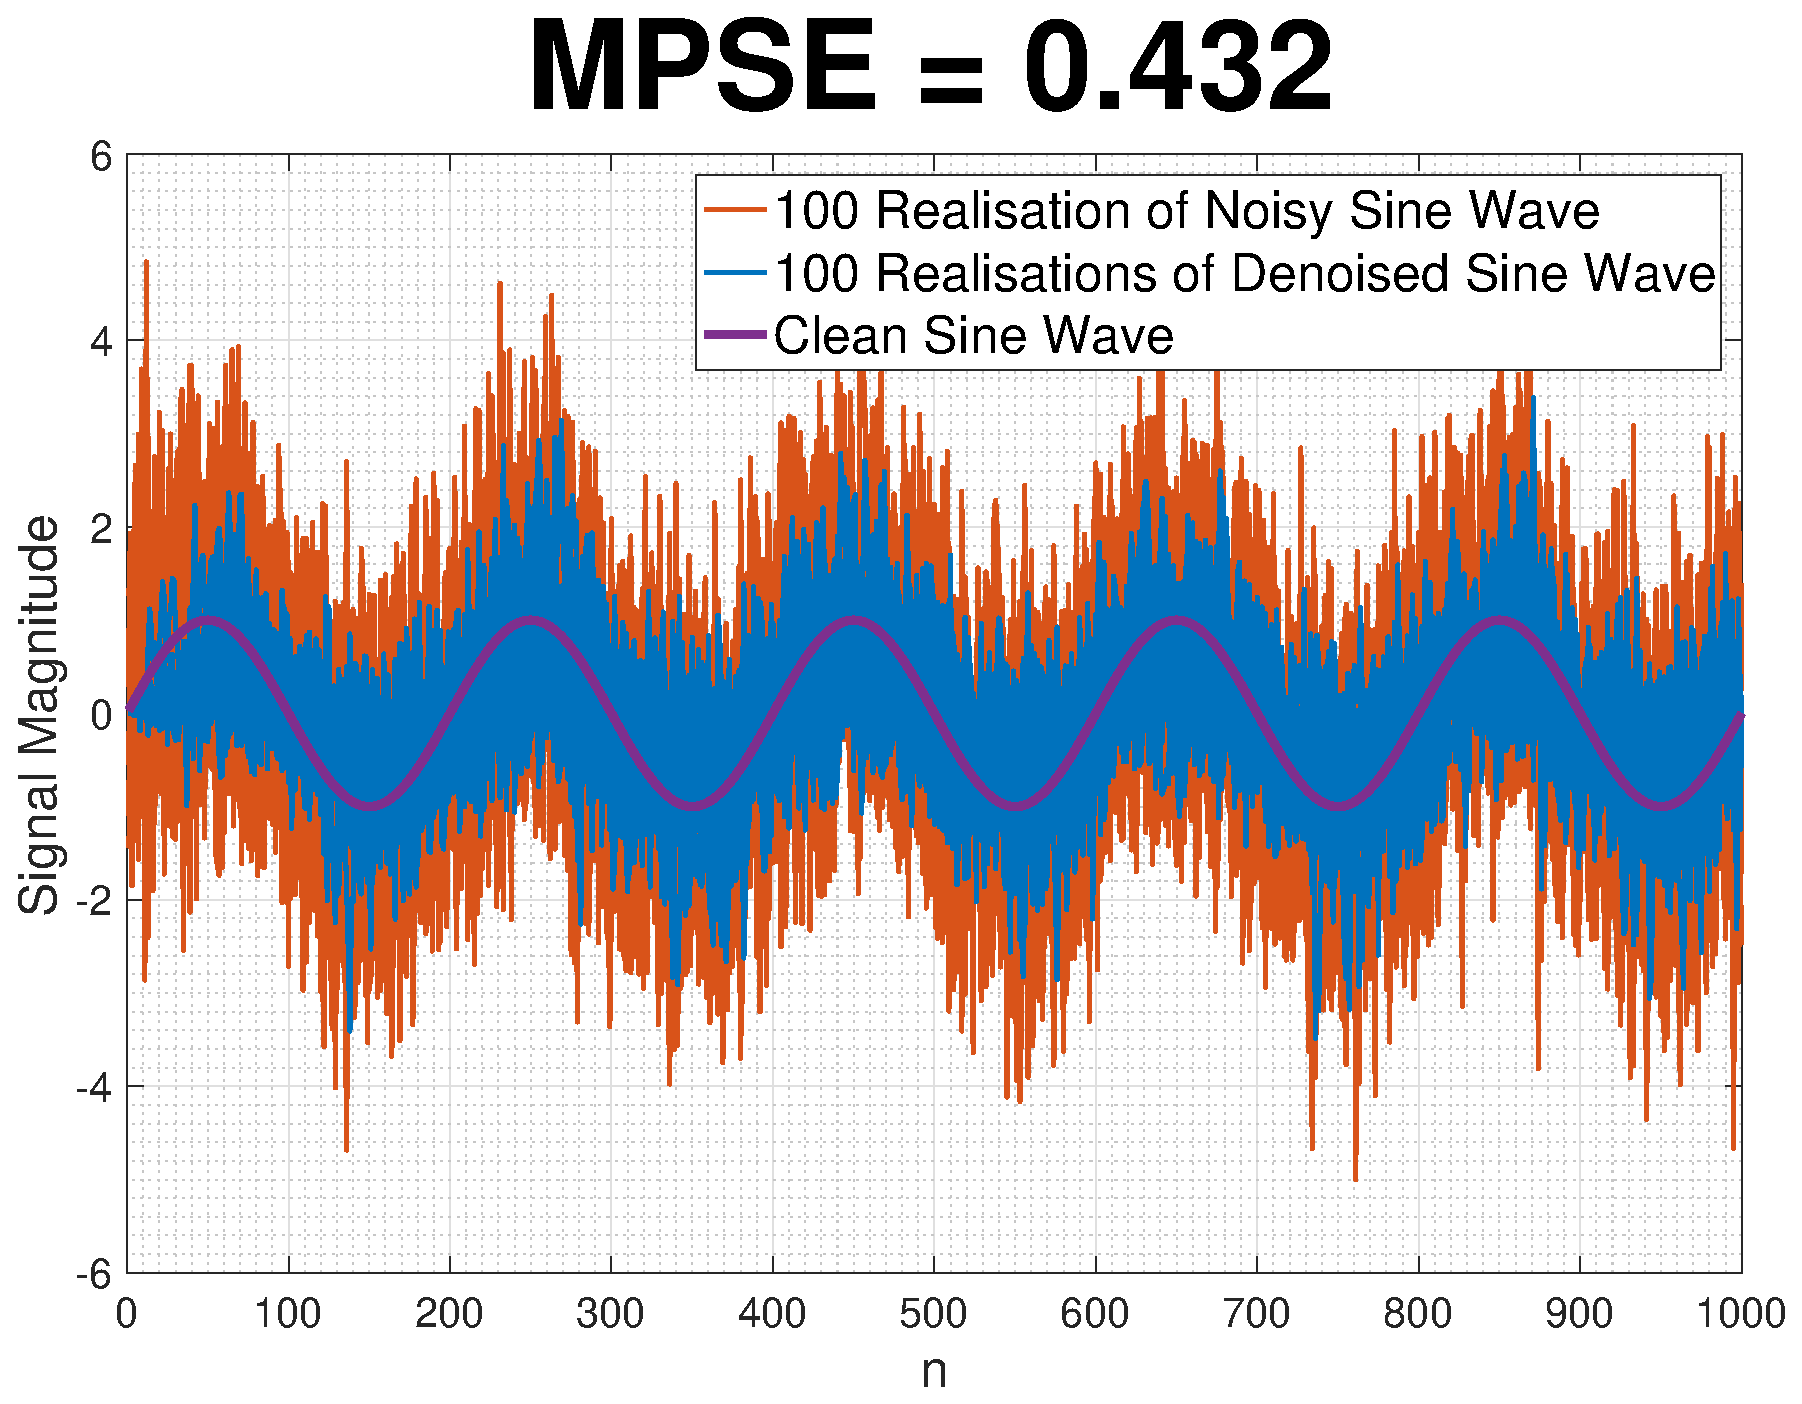
\includegraphics[width=0.24\textwidth]{part3/mpse_delay_2}
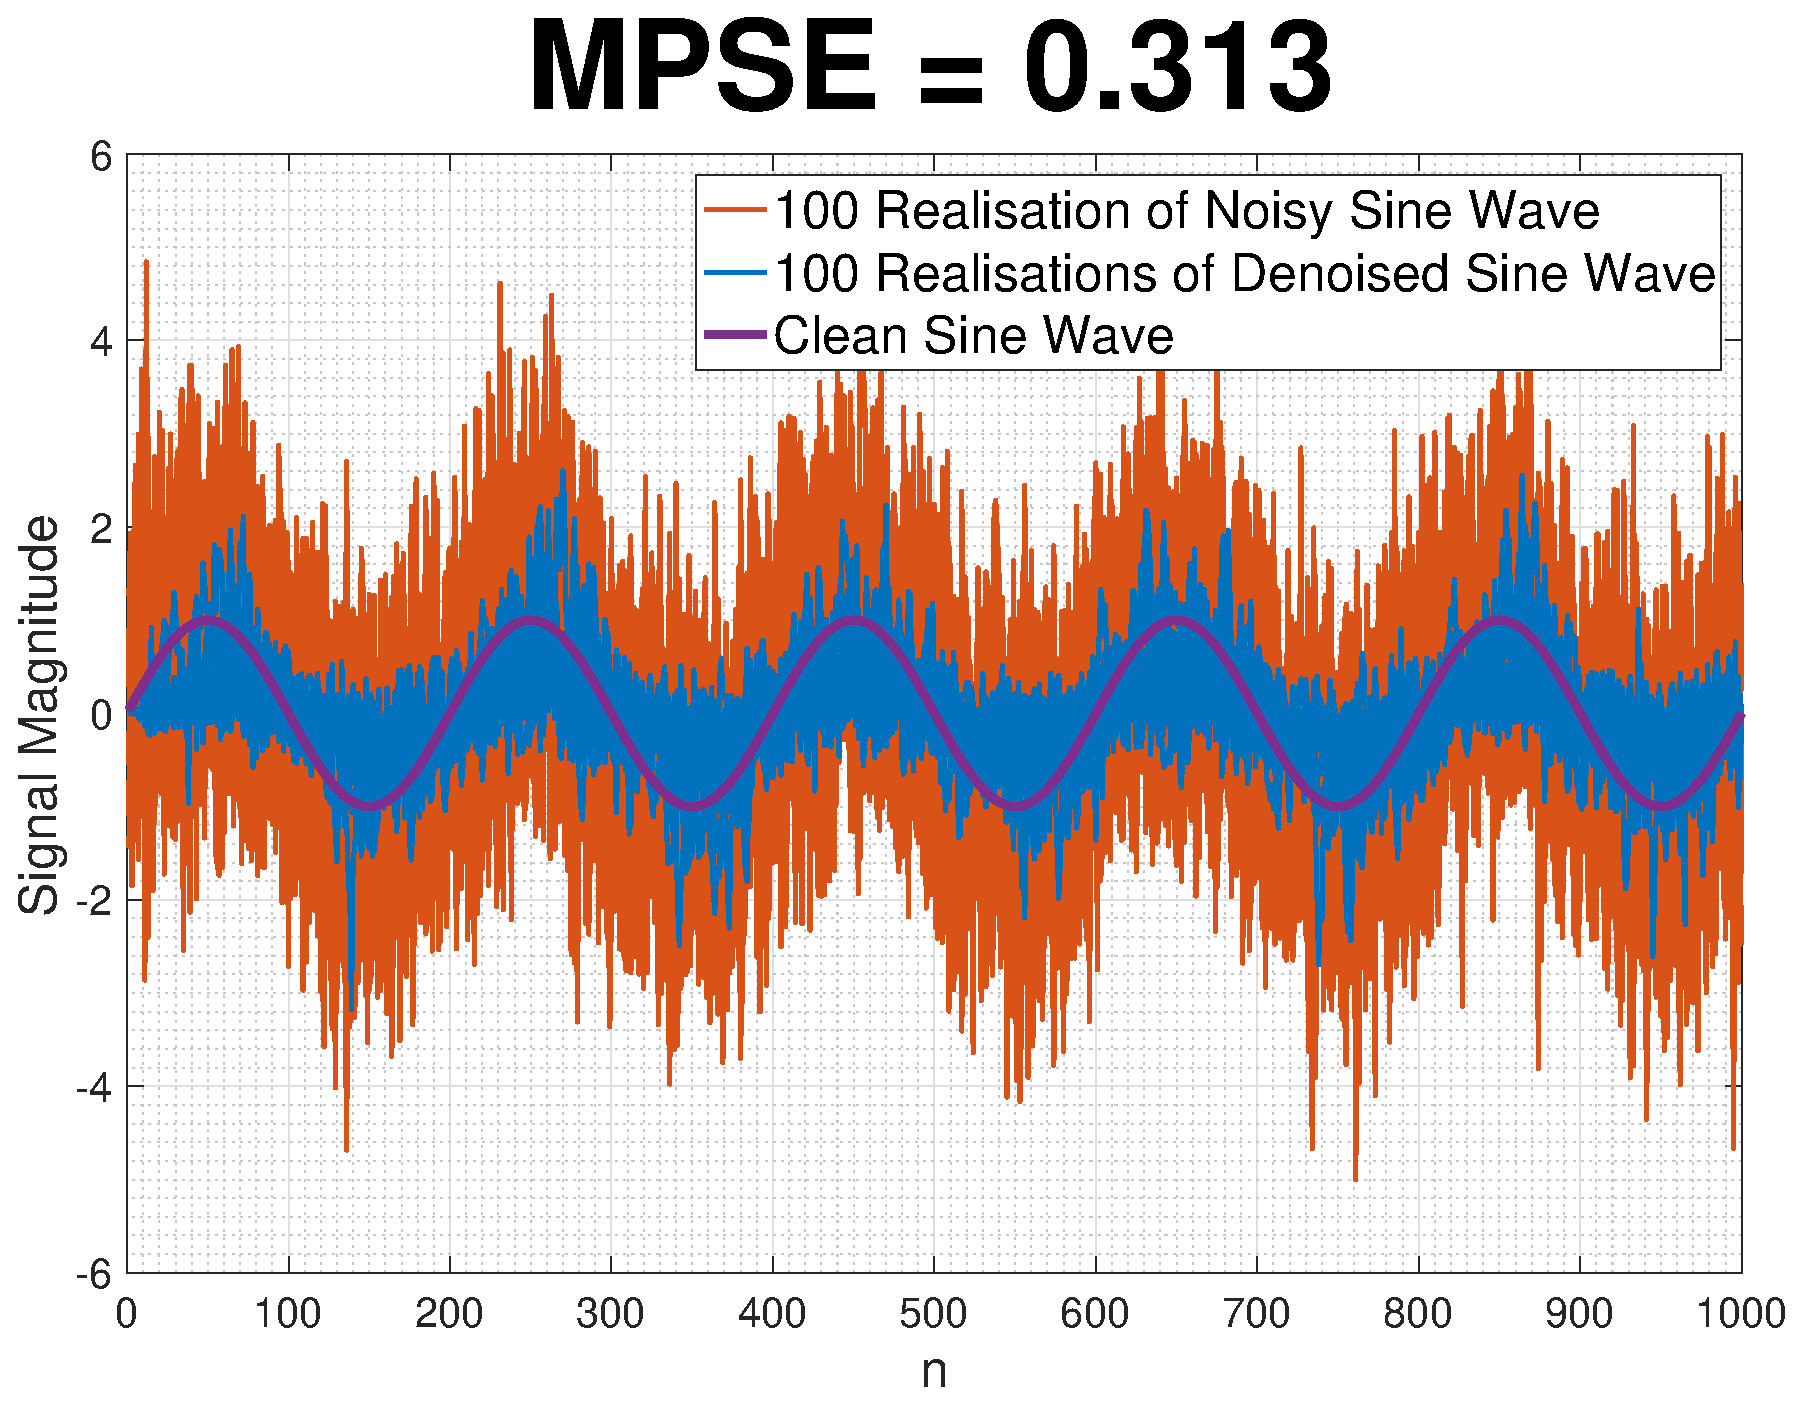
\includegraphics[width=0.24\textwidth]{part3/mpse_delay_3}
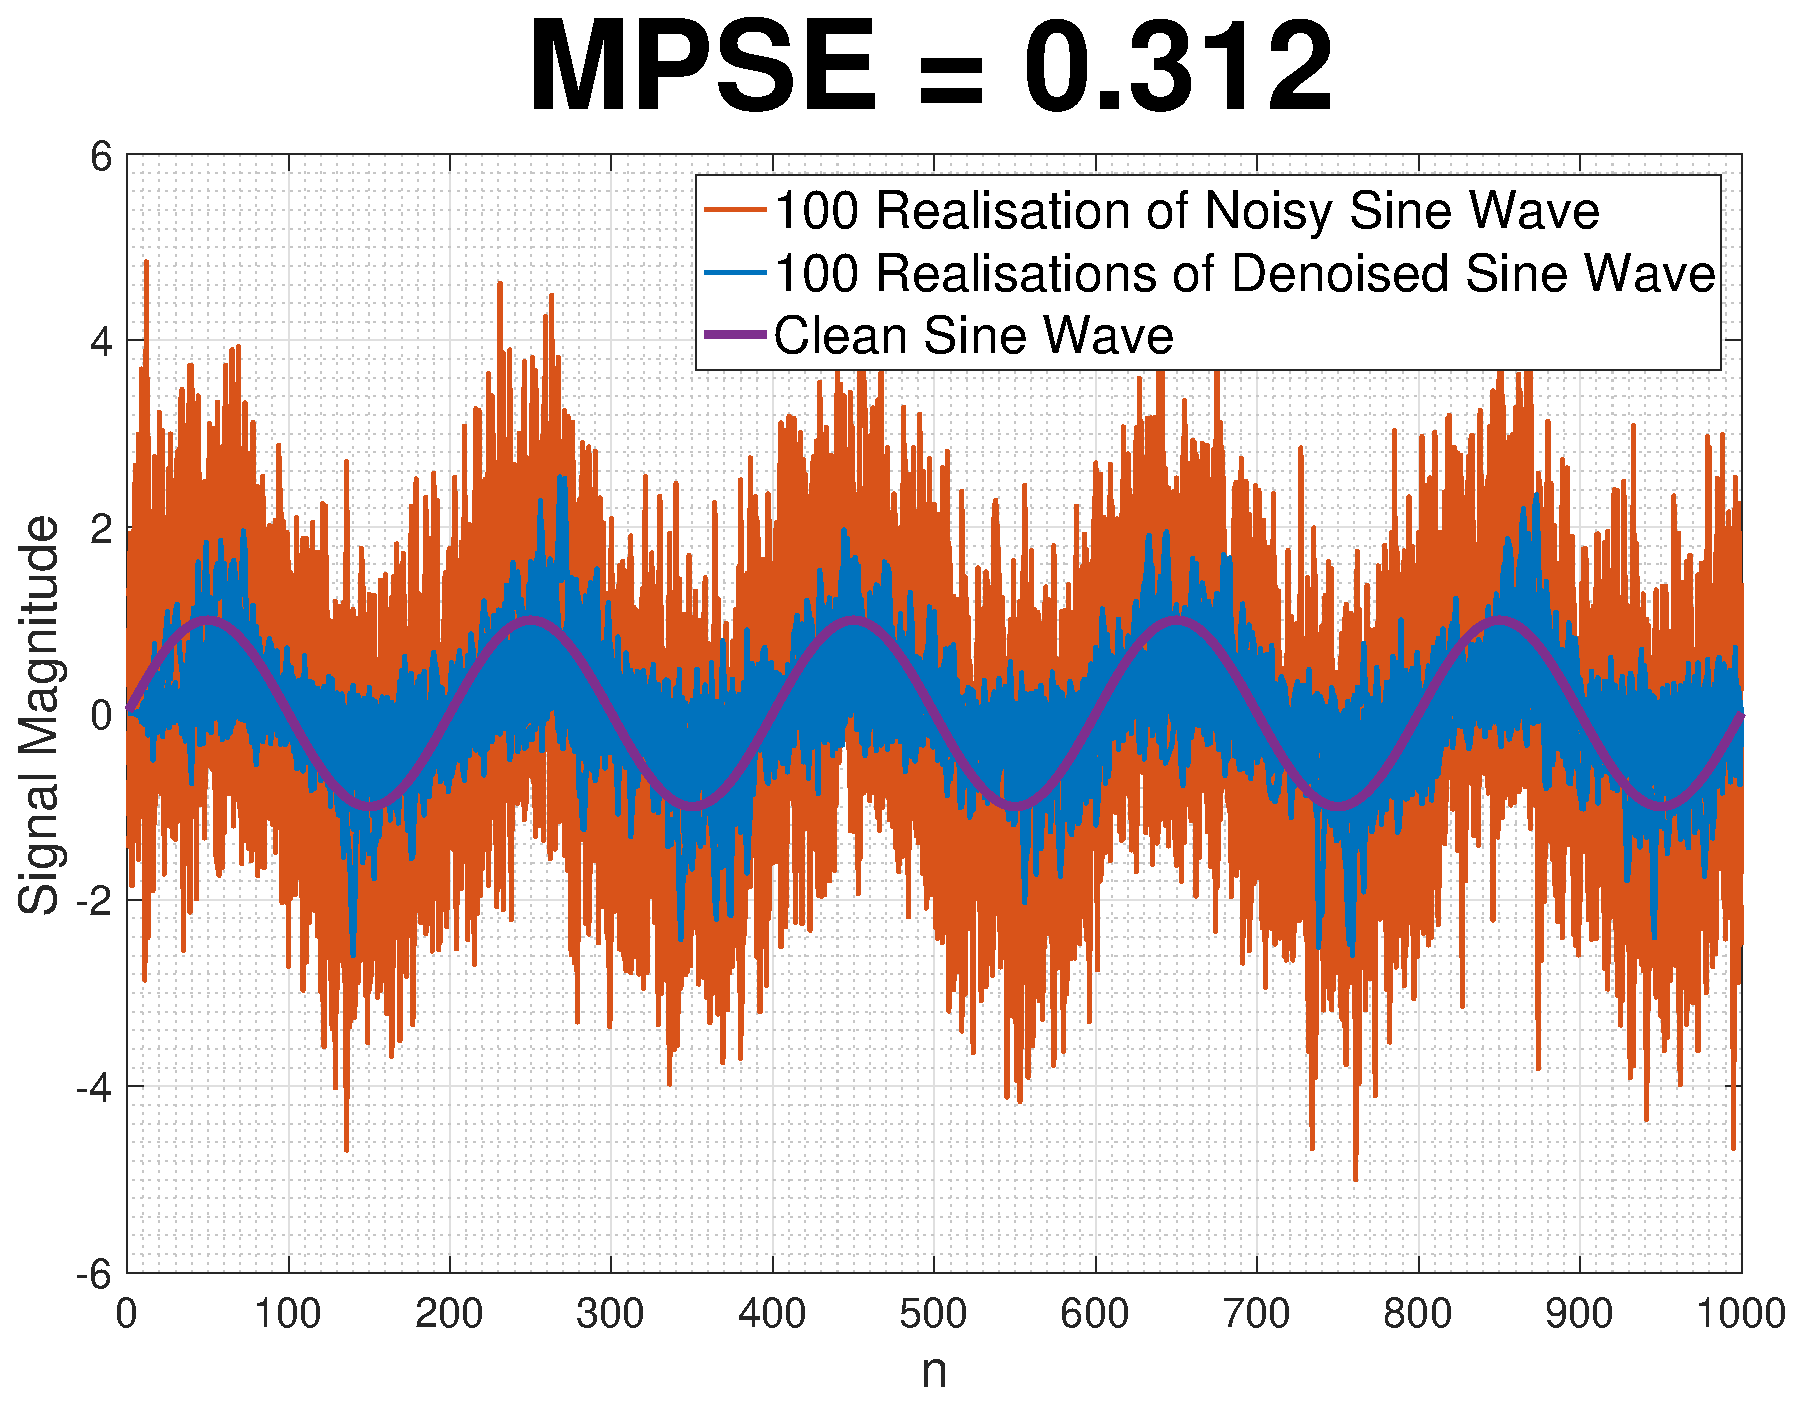
\includegraphics[width=0.24\textwidth]{part3/mpse_delay_4}
\caption{Determining Ideal Value for $\Delta$ to be used in the Adaptive Line Enhancement Algorithm}
\end{figure}

\begin{figure}[H]
\centering{}
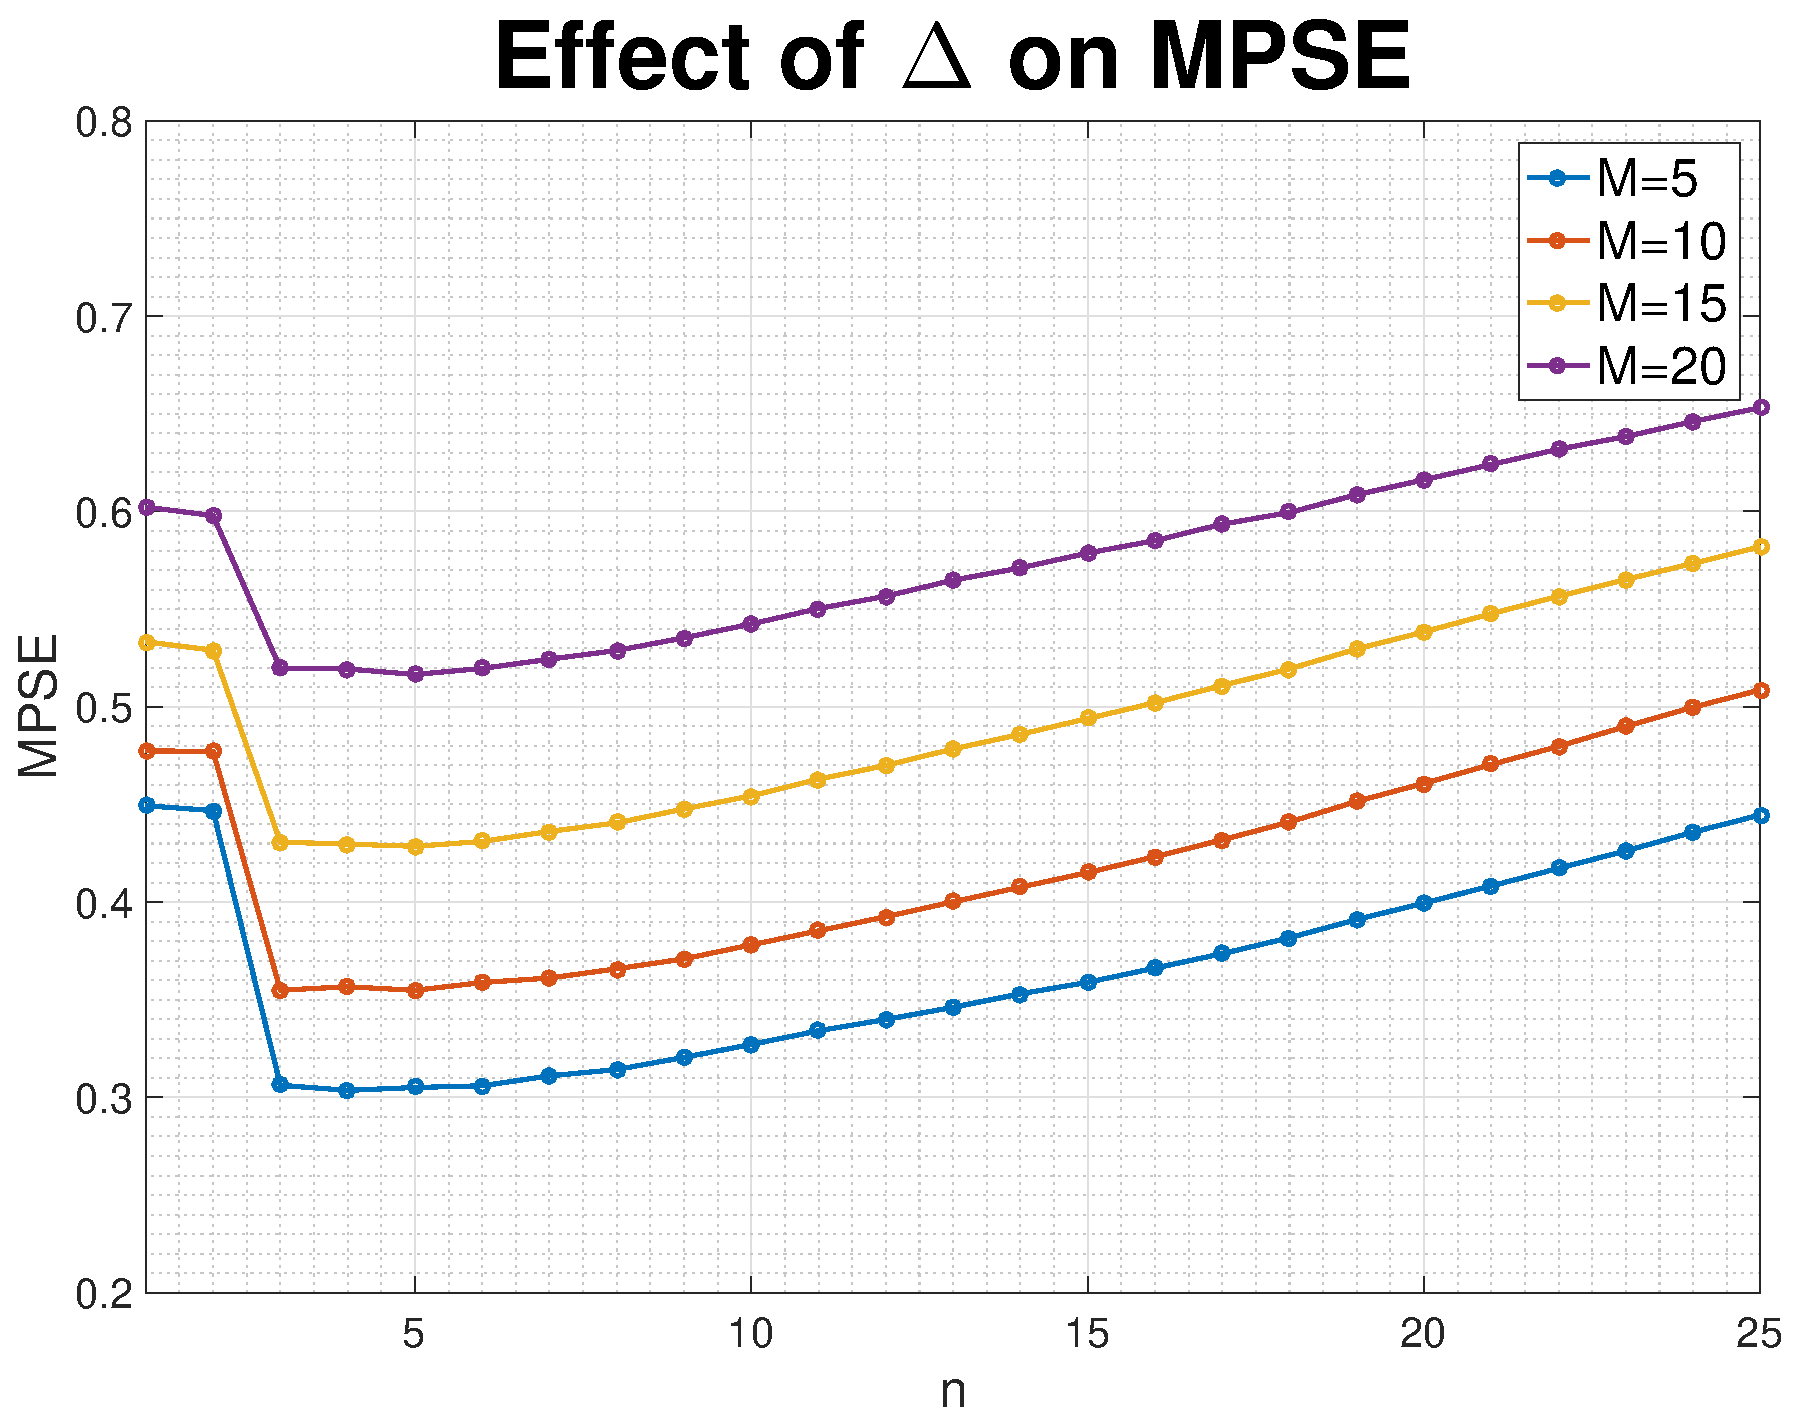
\includegraphics[width=0.32\textwidth]{part3/delay_vs_mpse}
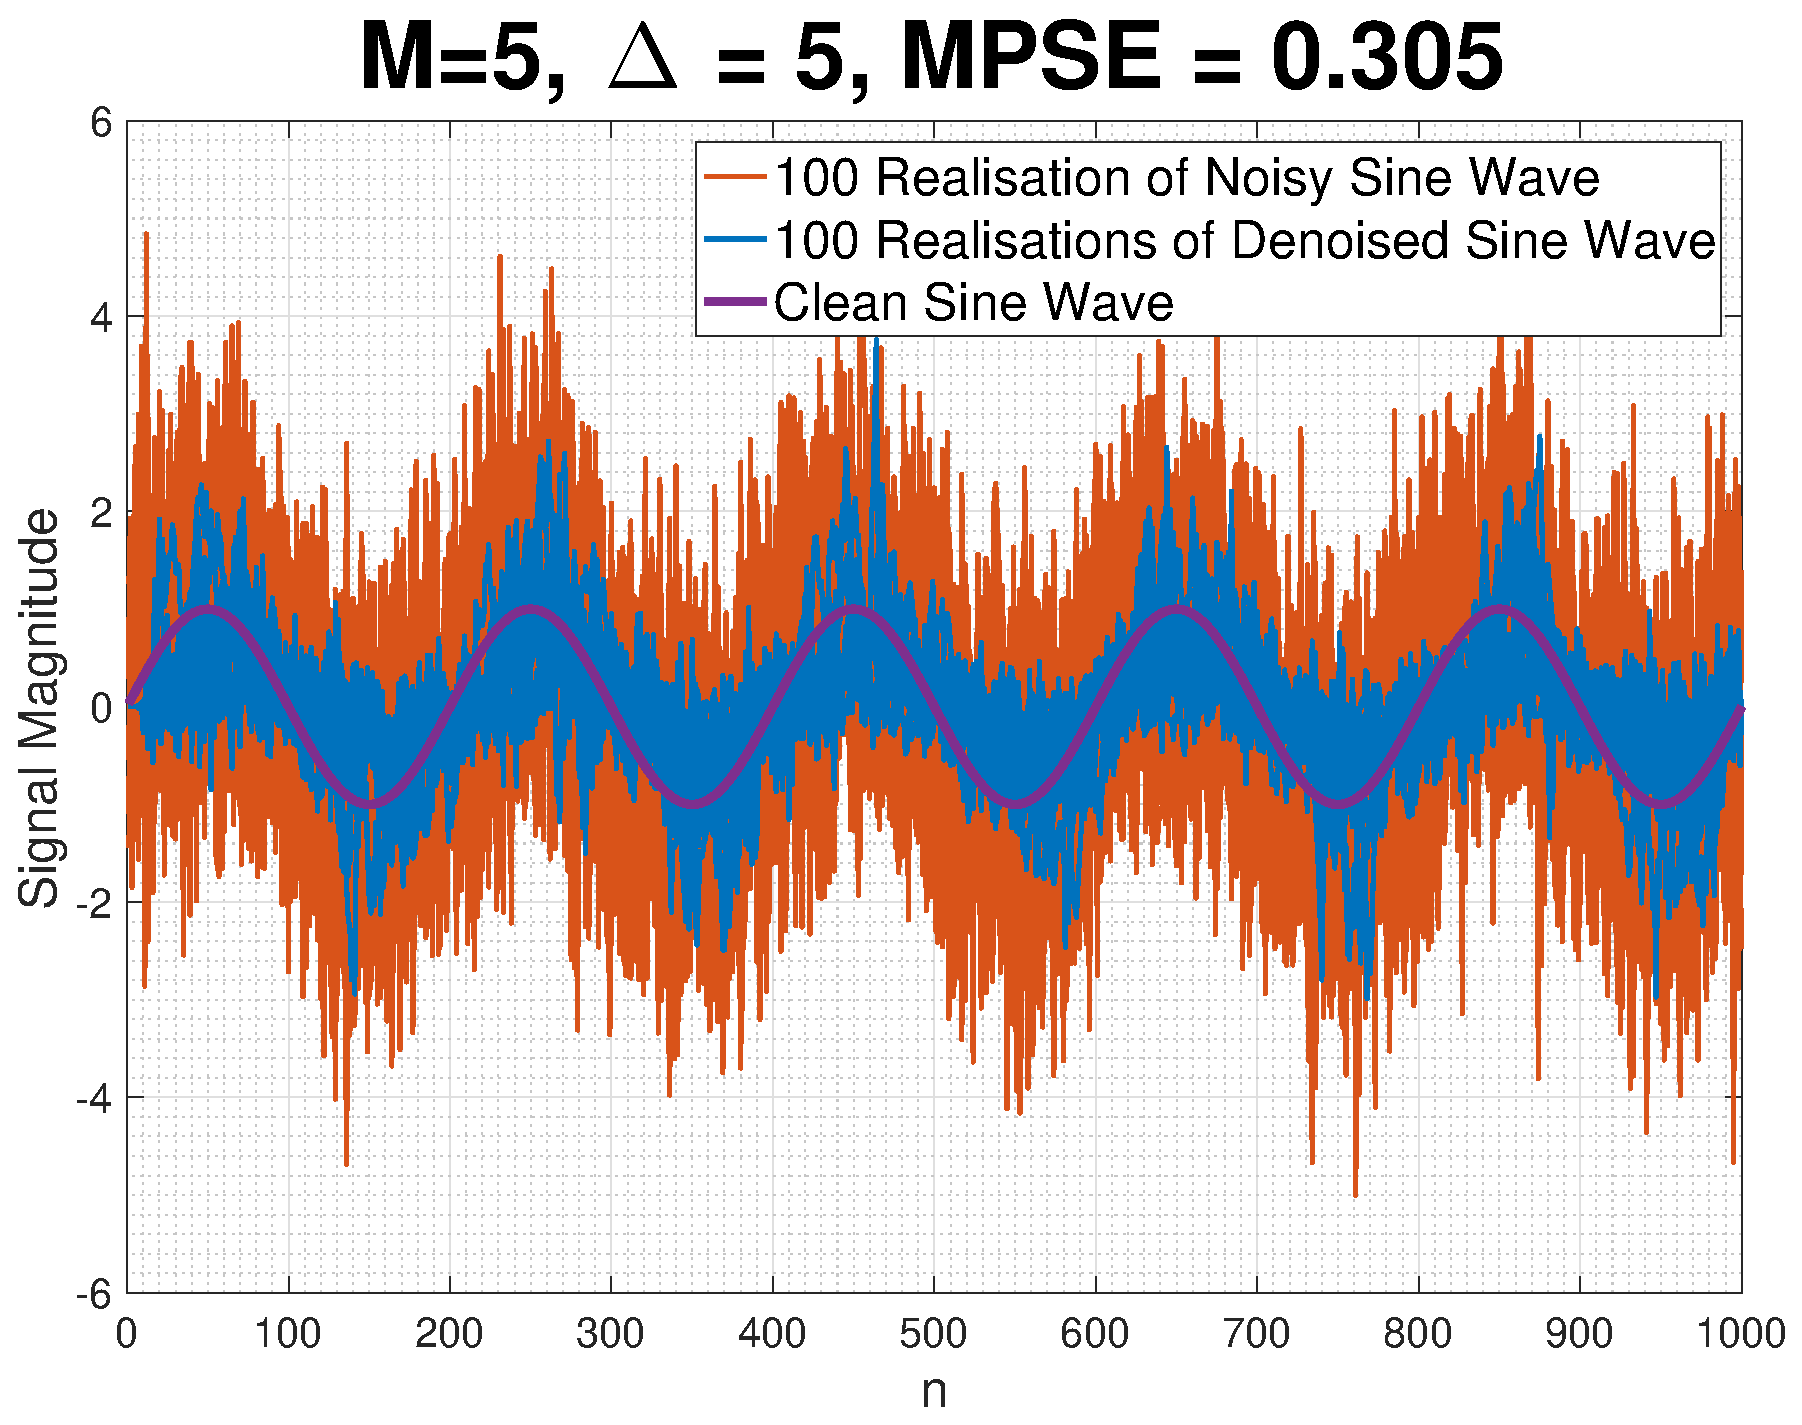
\includegraphics[width=0.32\textwidth]{part3/mpse_delay_5}
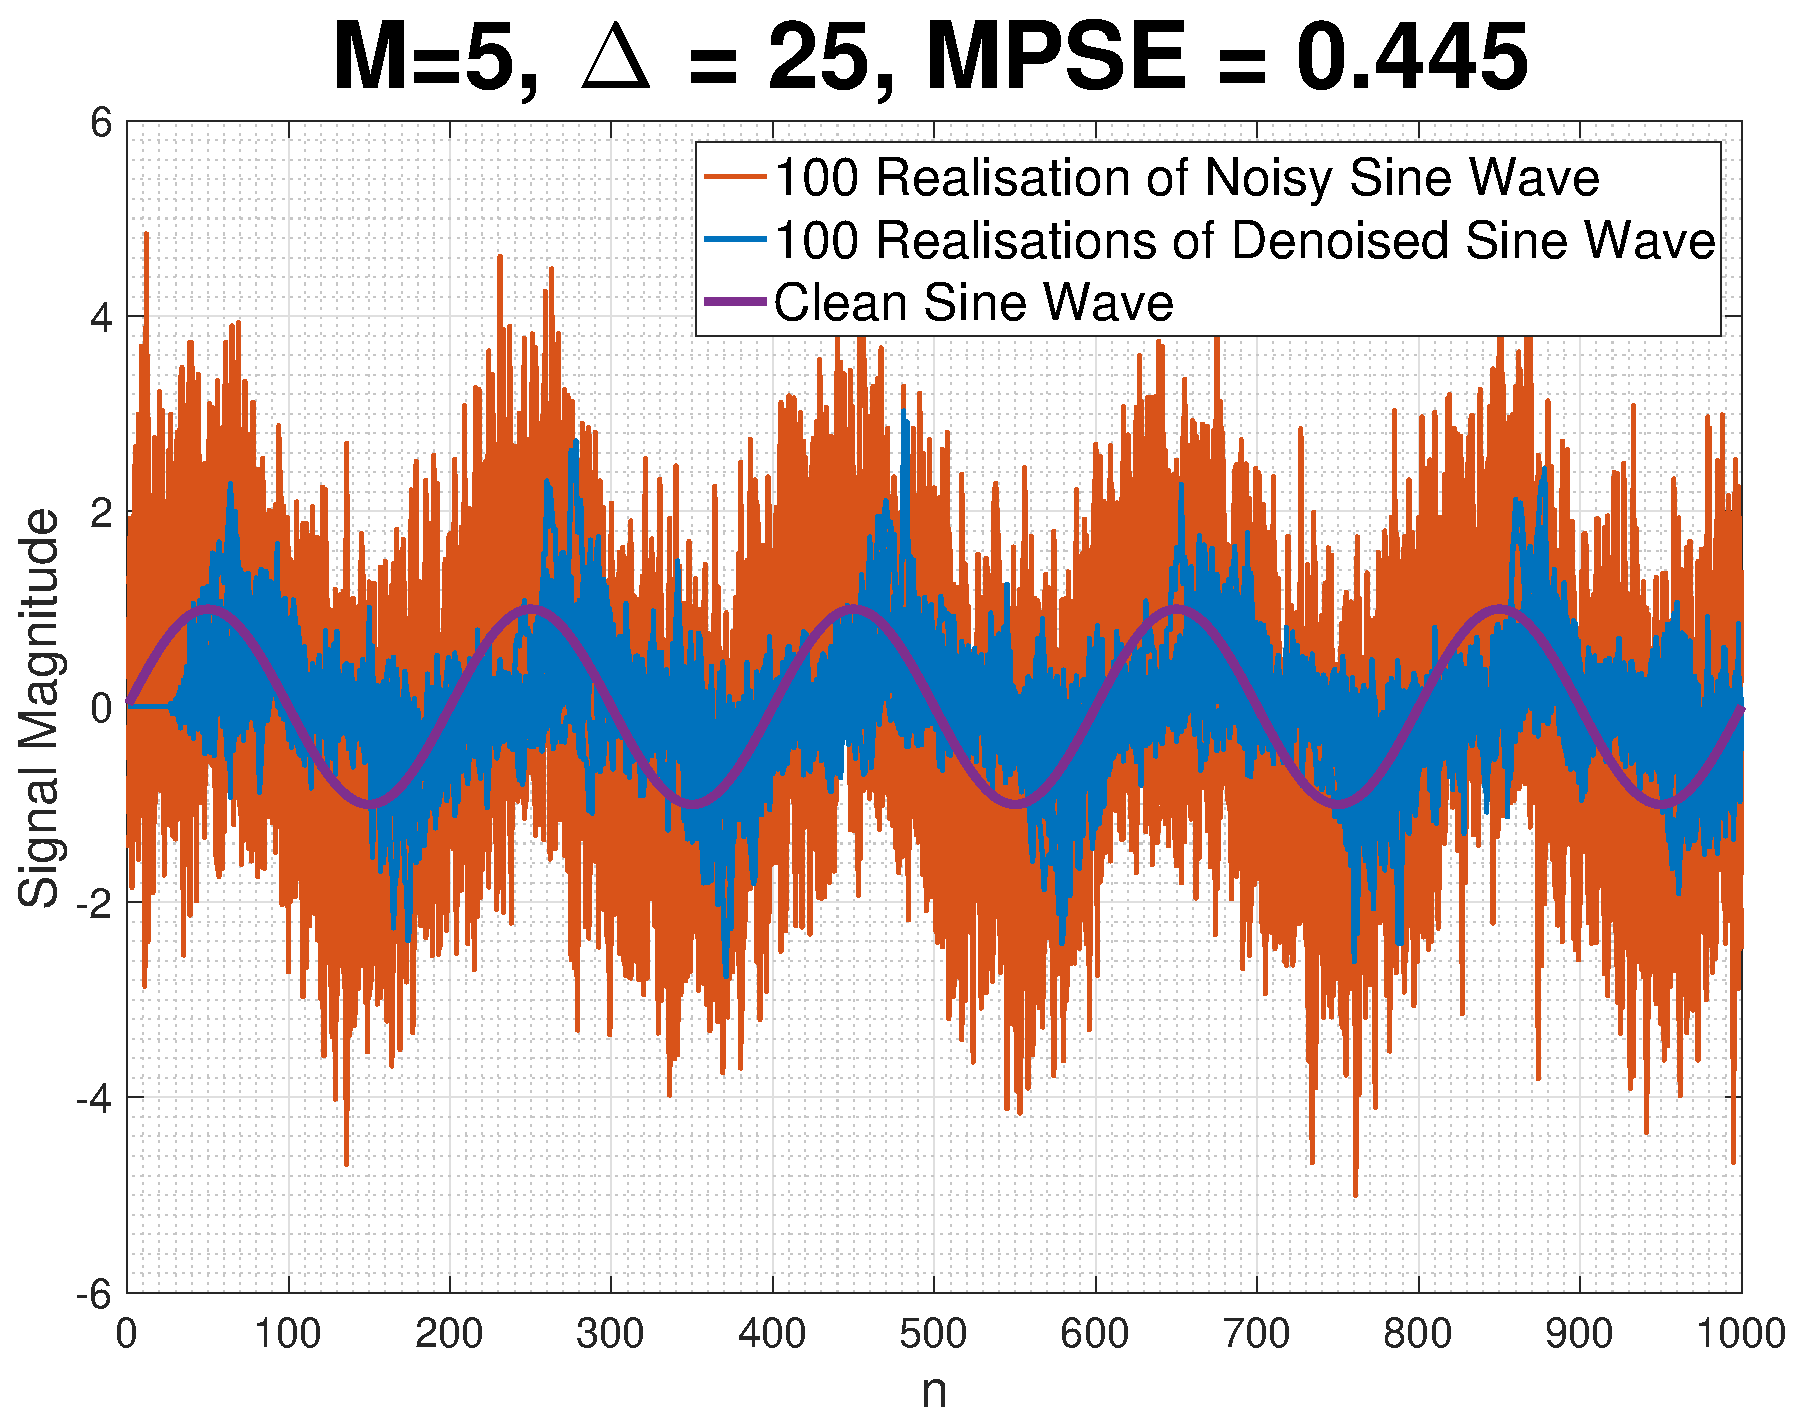
\includegraphics[width=0.32\textwidth]{part3/mpse_delay_25}
\caption{Studying the Effects of Increasing Delay on the MPSE}
\end{figure}

\begin{figure}[H]
\centering{}
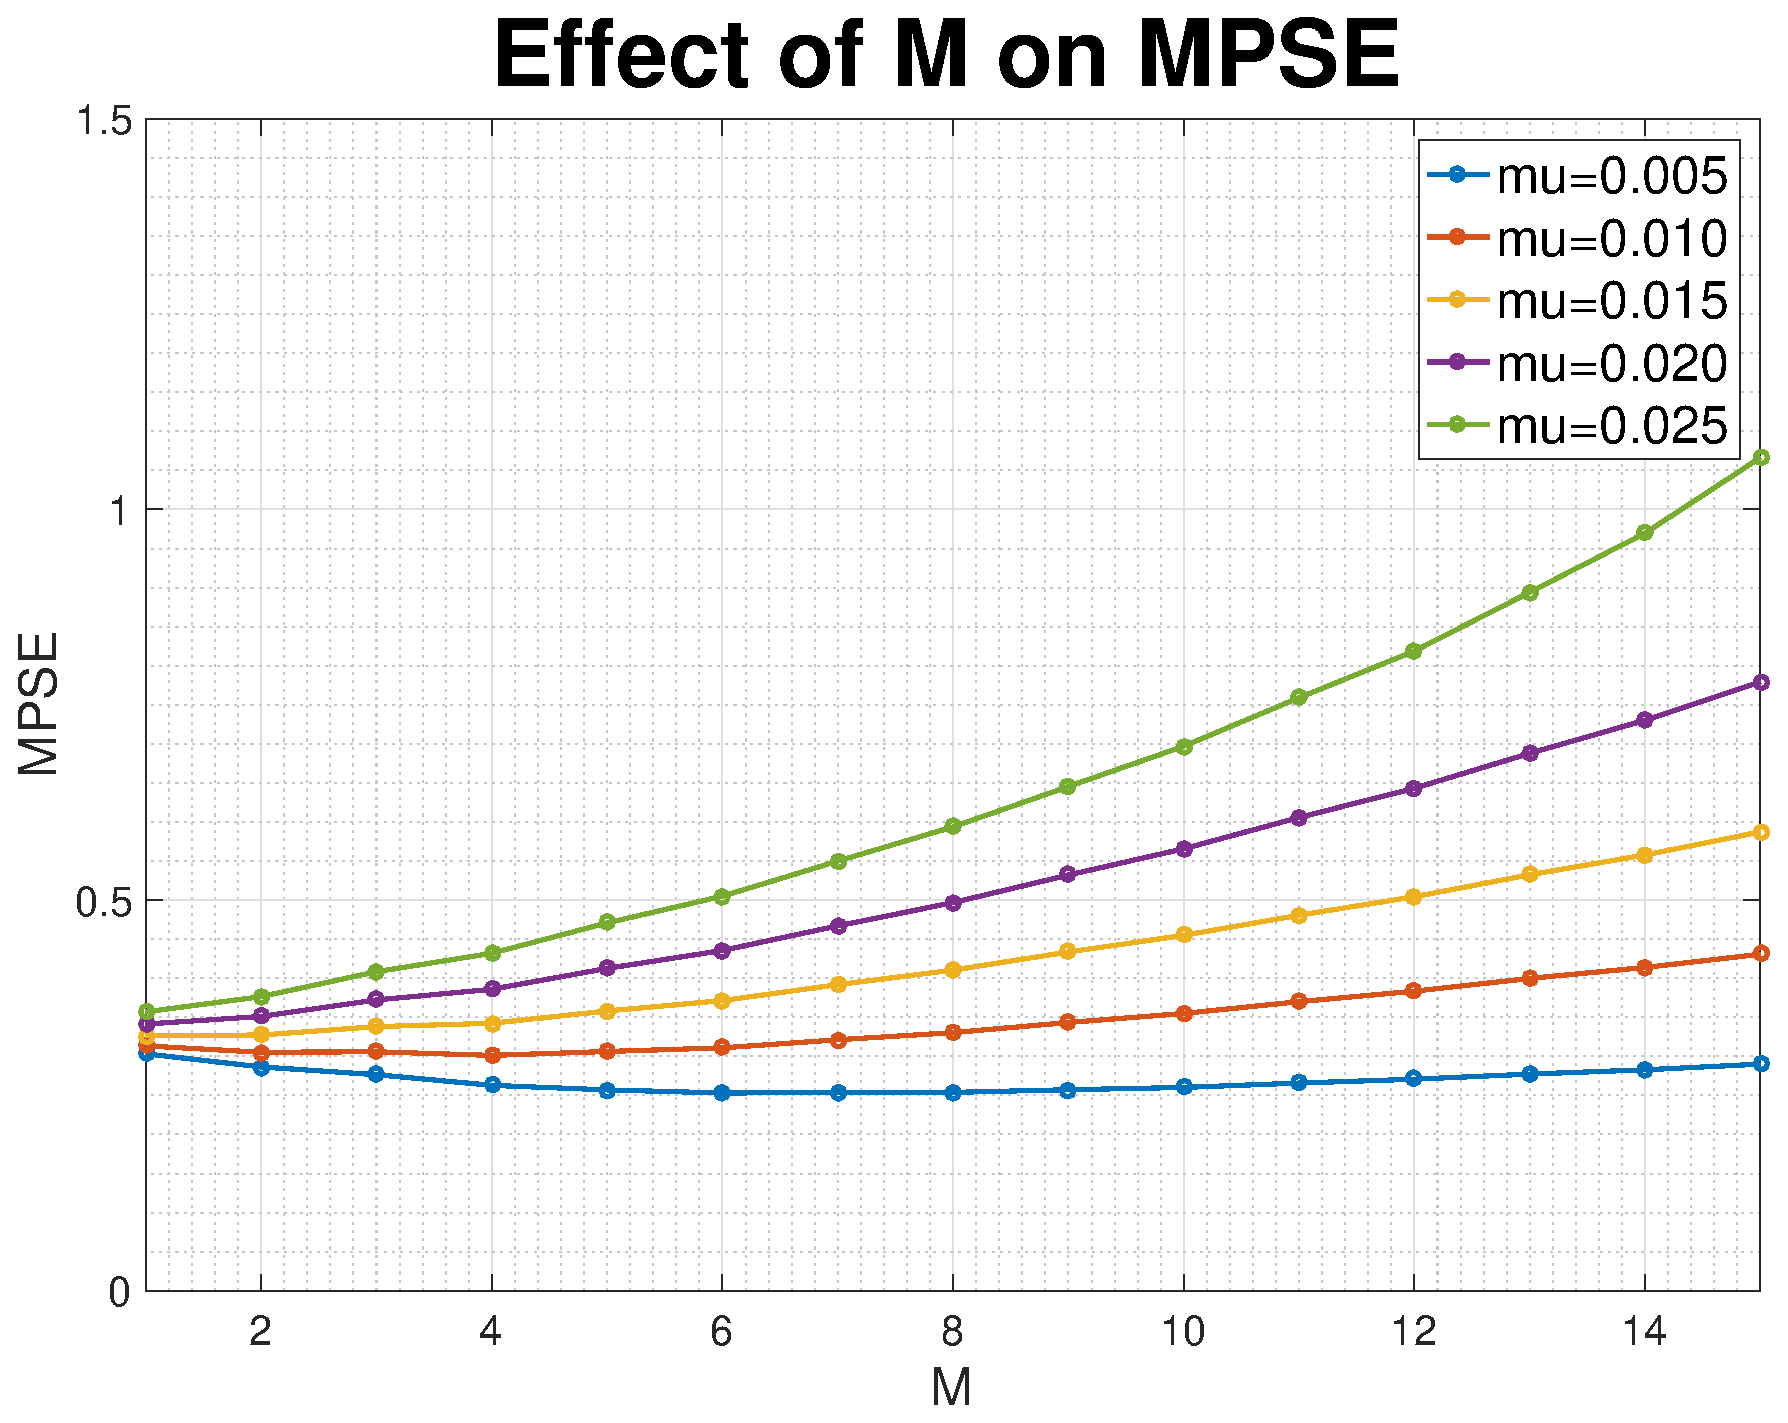
\includegraphics[width=0.32\textwidth]{part3/model_order_mpse}
\caption{Studying the Effects of Increasing Model Order on the MPSE}
\end{figure}

\begin{figure}[H]
\centering{}
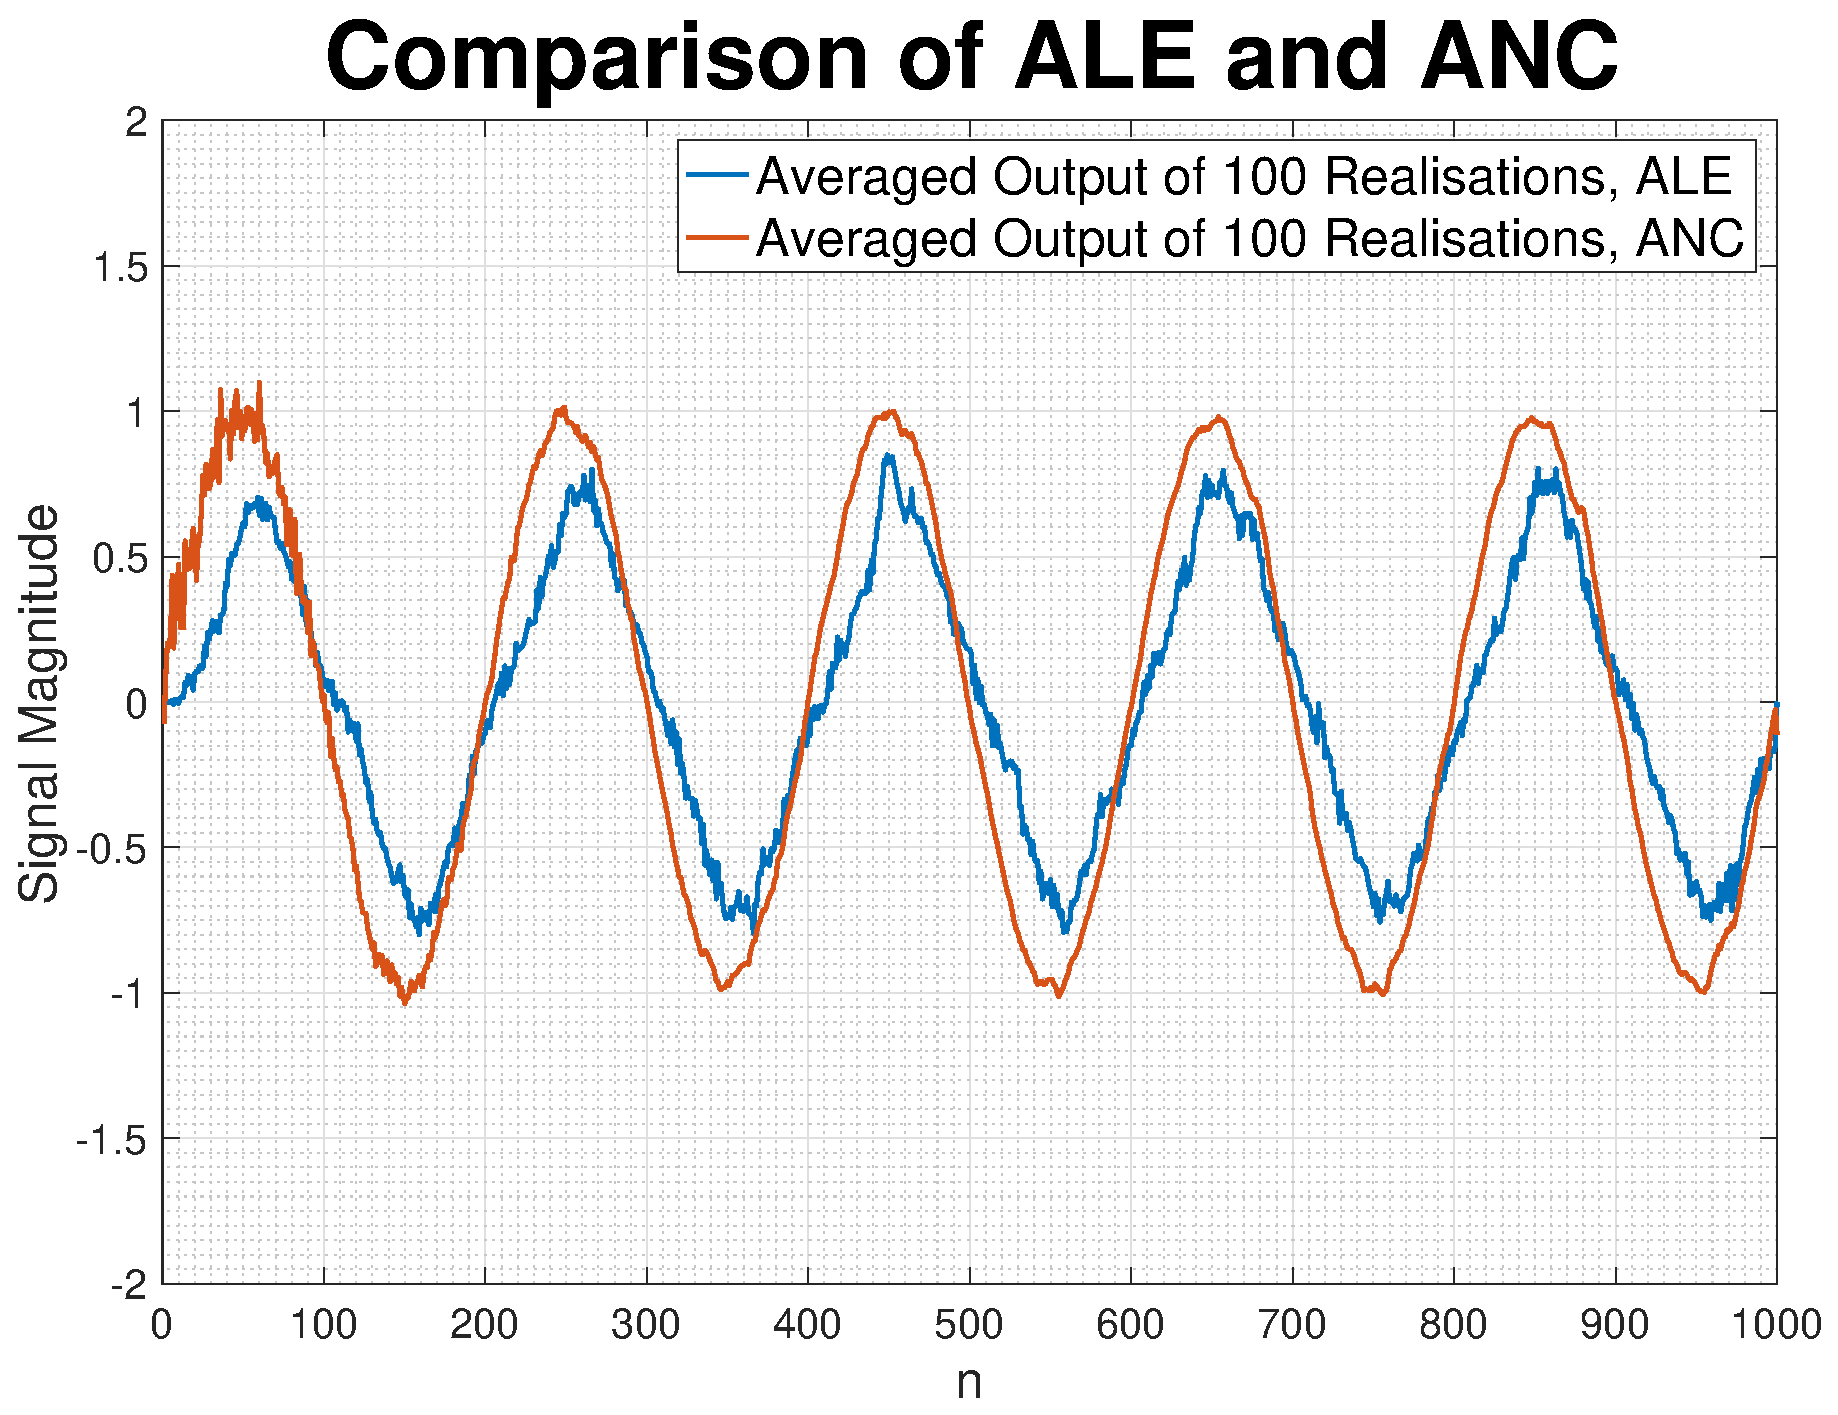
\includegraphics[width=0.32\textwidth]{part3/anc_ale_comparison}
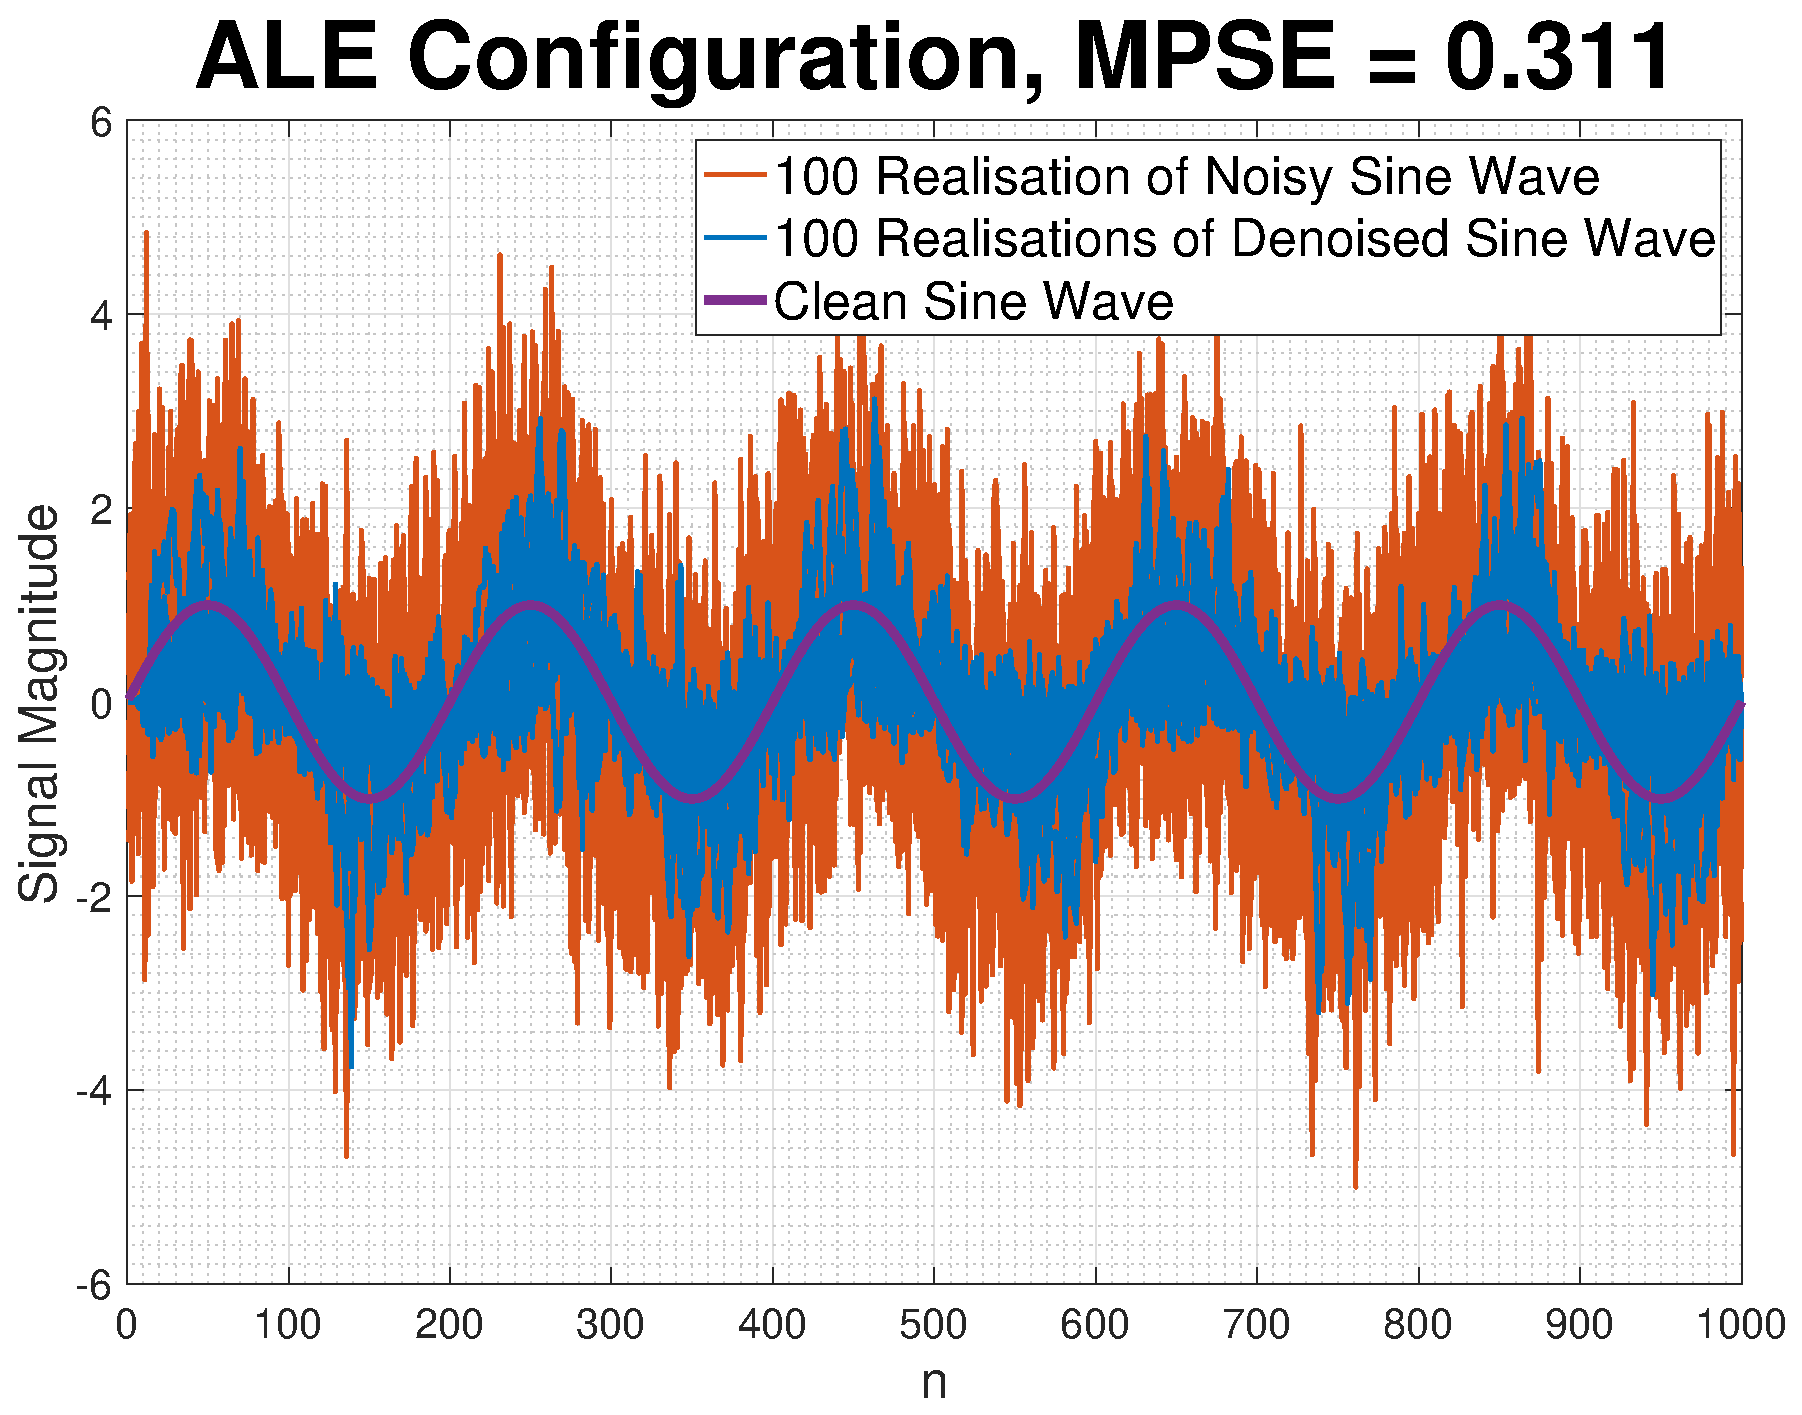
\includegraphics[width=0.32\textwidth]{part3/ale_mpse}
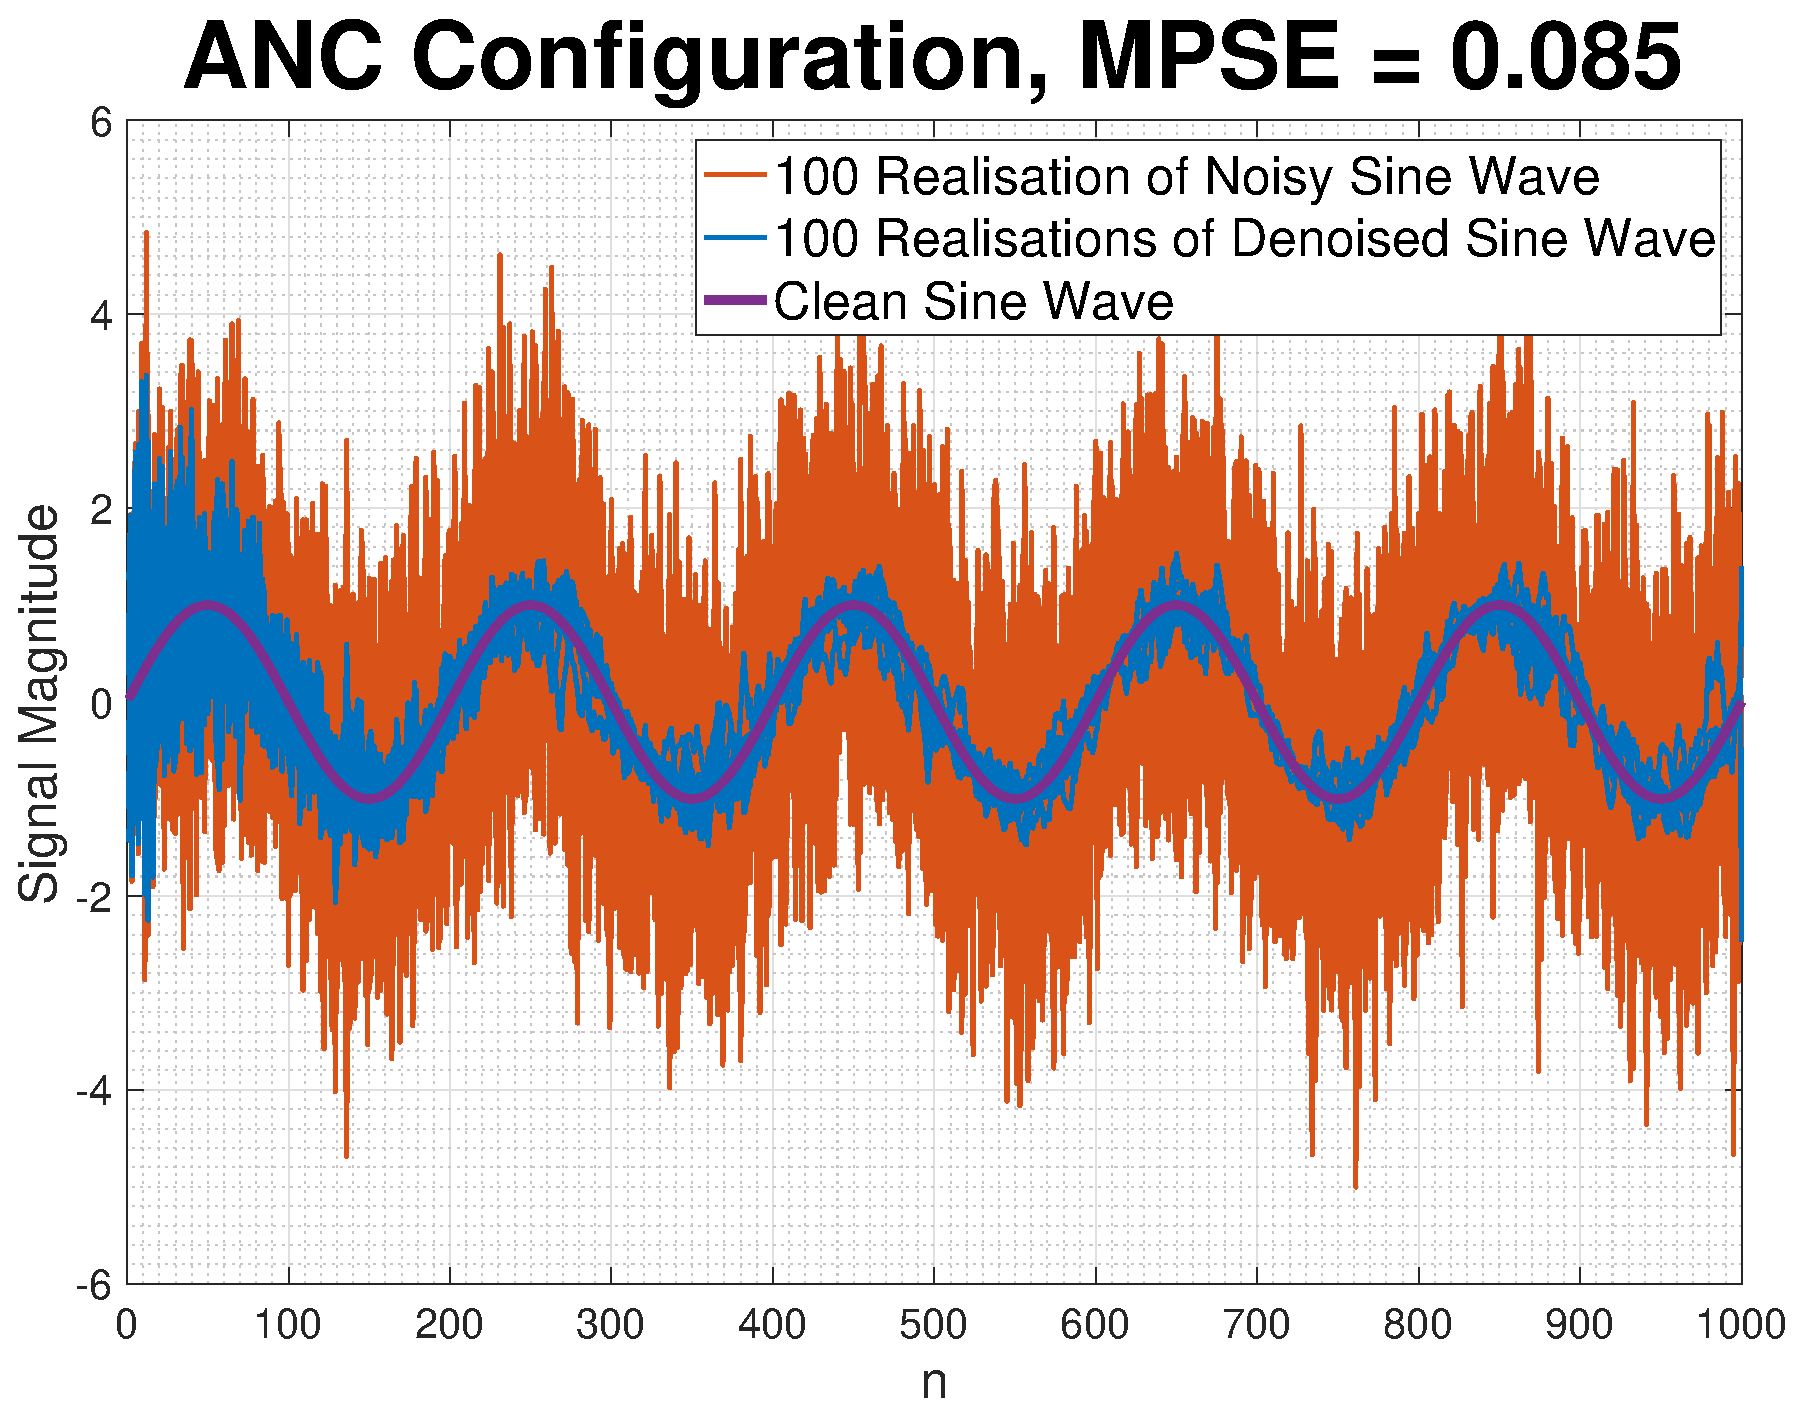
\includegraphics[width=0.32\textwidth]{part3/anc_mpse}
\caption{Comparison of ALE and ANC Configurations for Denoising Sinewave}
\end{figure}

\begin{figure}[H]
\centering{}
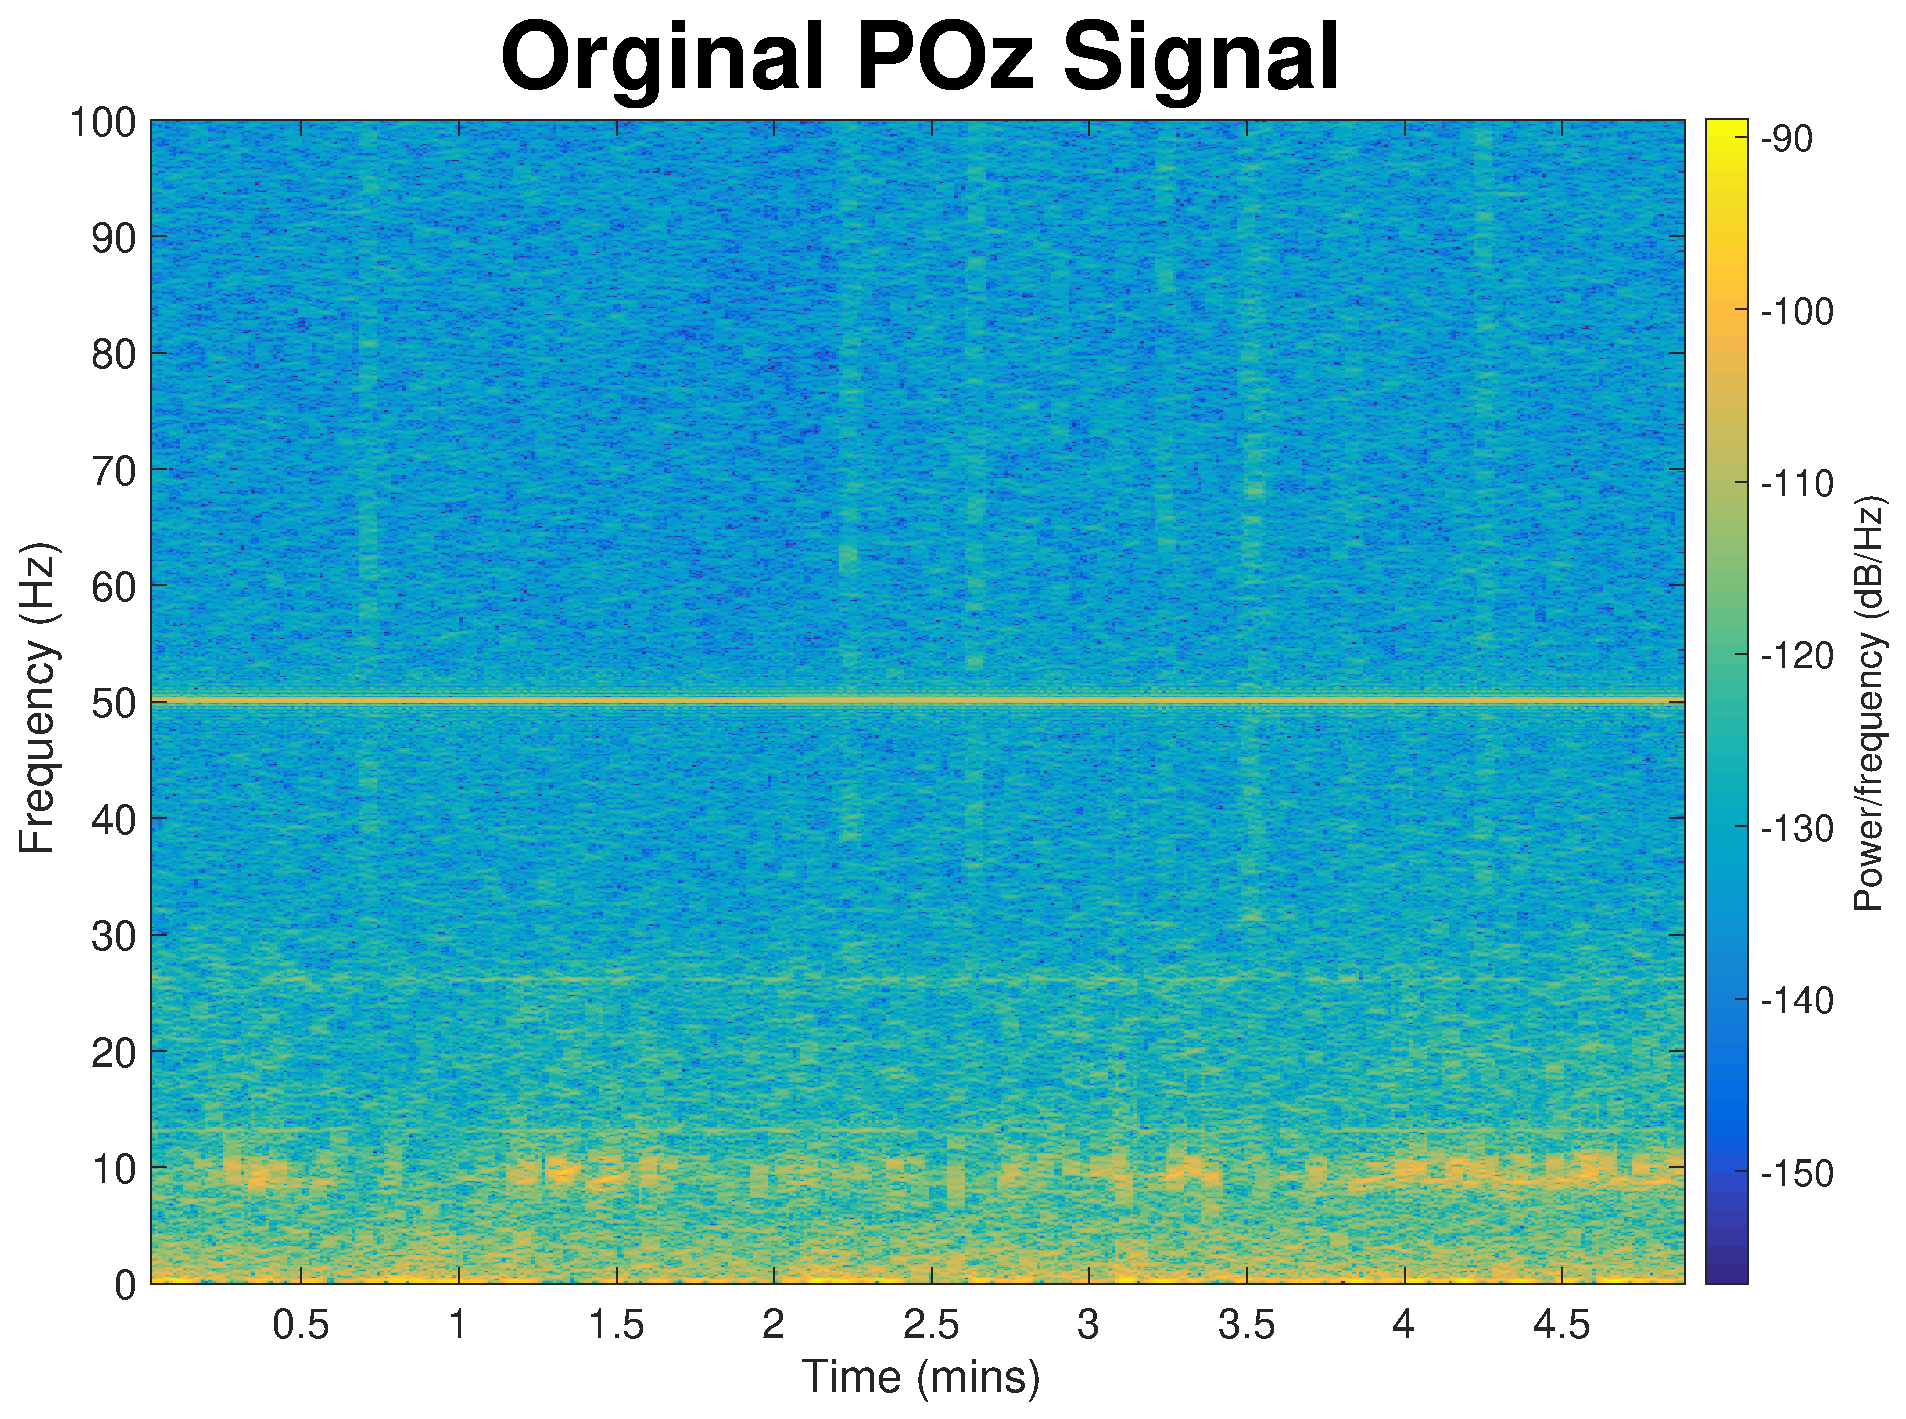
\includegraphics[width=0.32\textwidth]{part3/original_POz_spectrogram}
\caption{Original EEG Data collected from POz Location on the Scalp with Strong Component at 50 Hz}
\end{figure}


\begin{figure}[H]
\centering{}
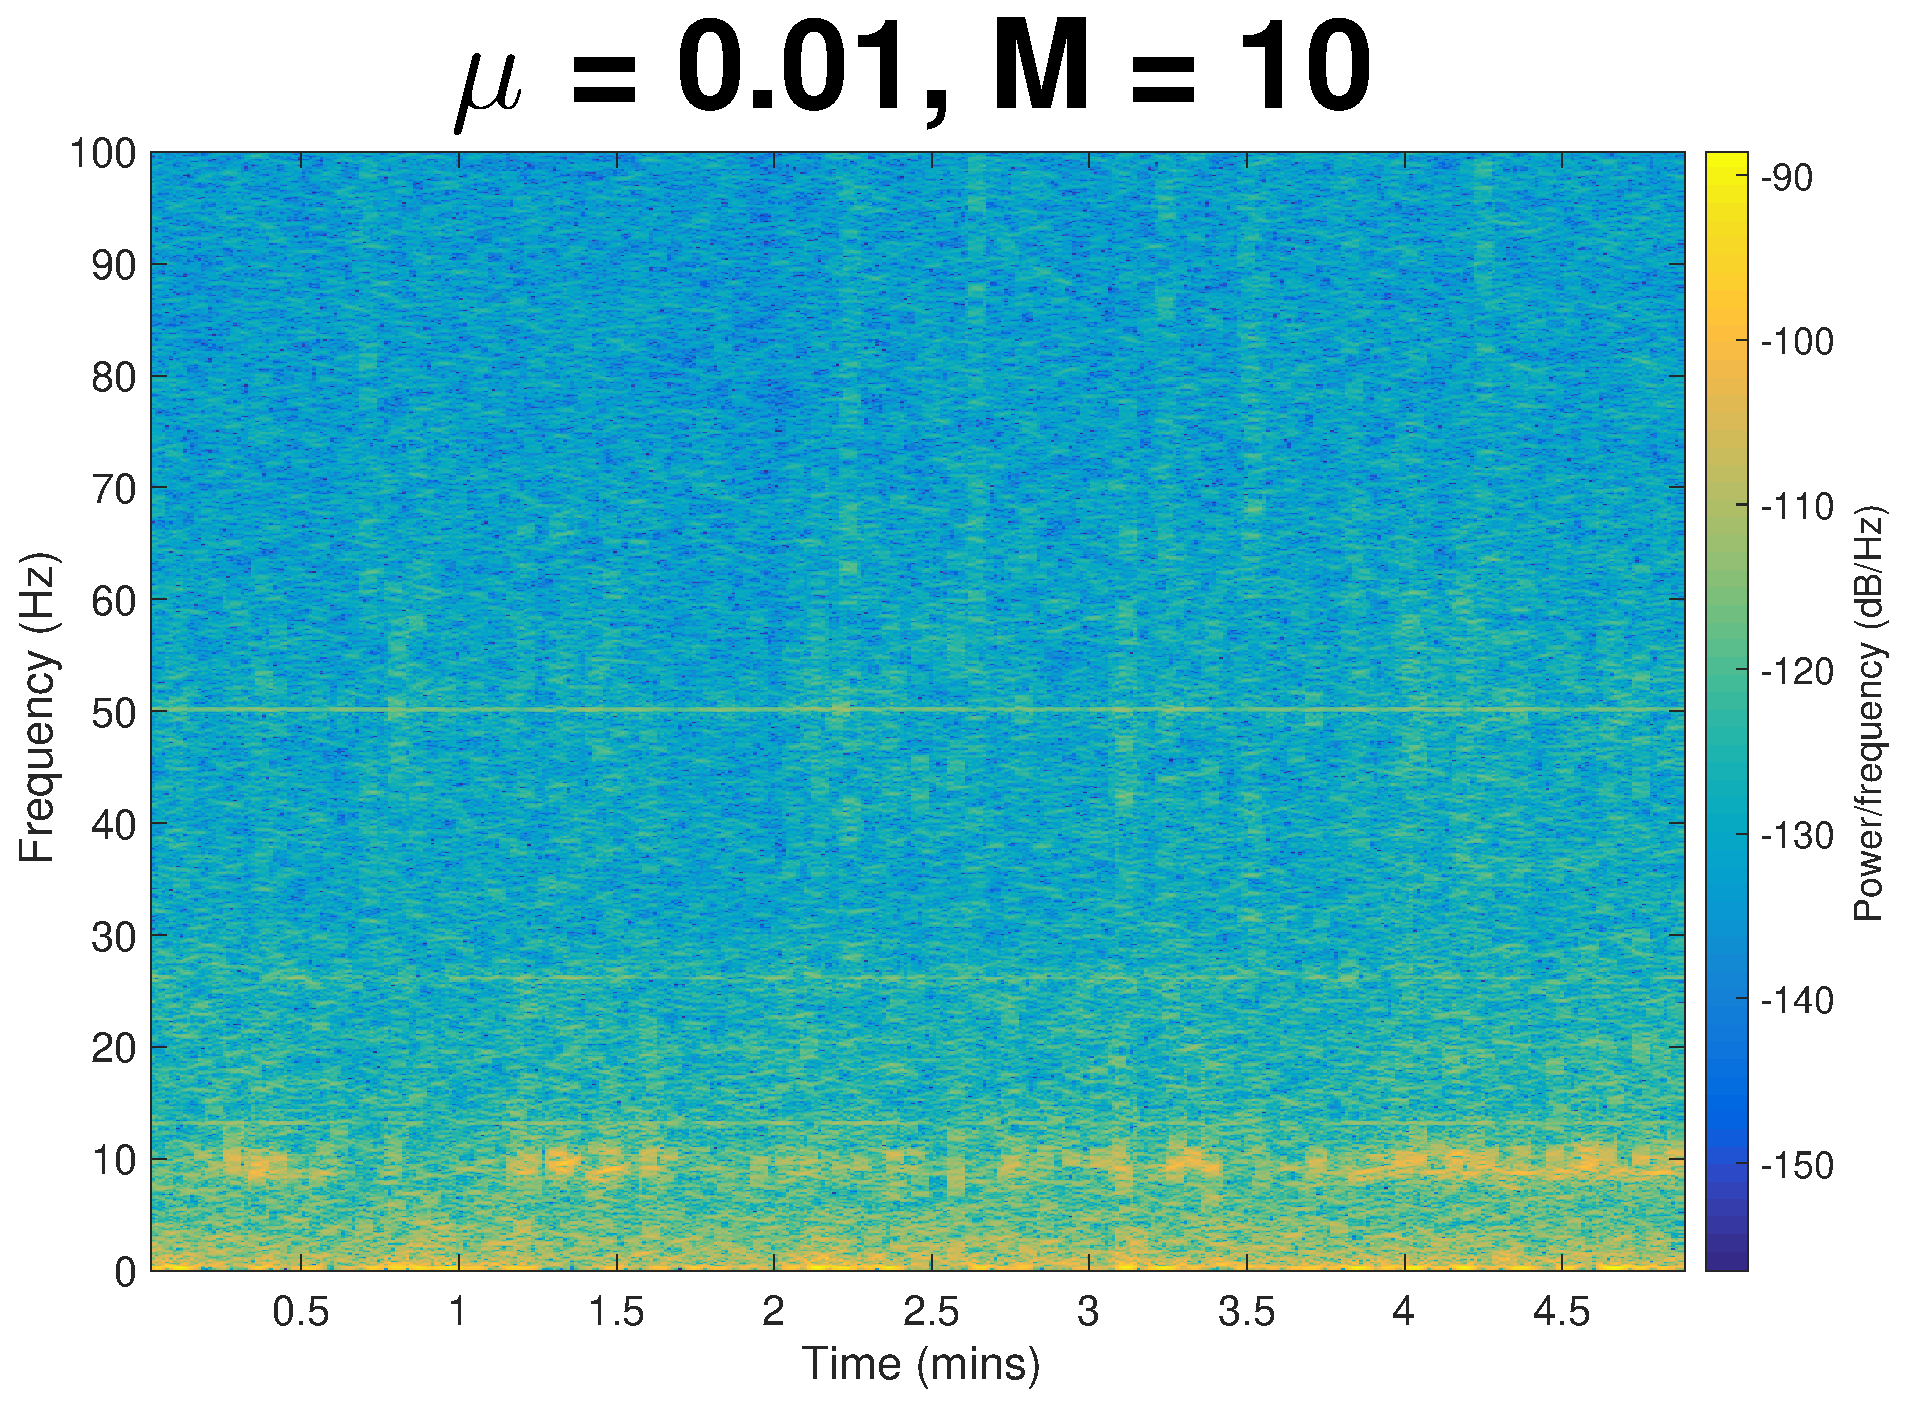
\includegraphics[width=0.24\textwidth]{part3/POz_mu_01_M_10}
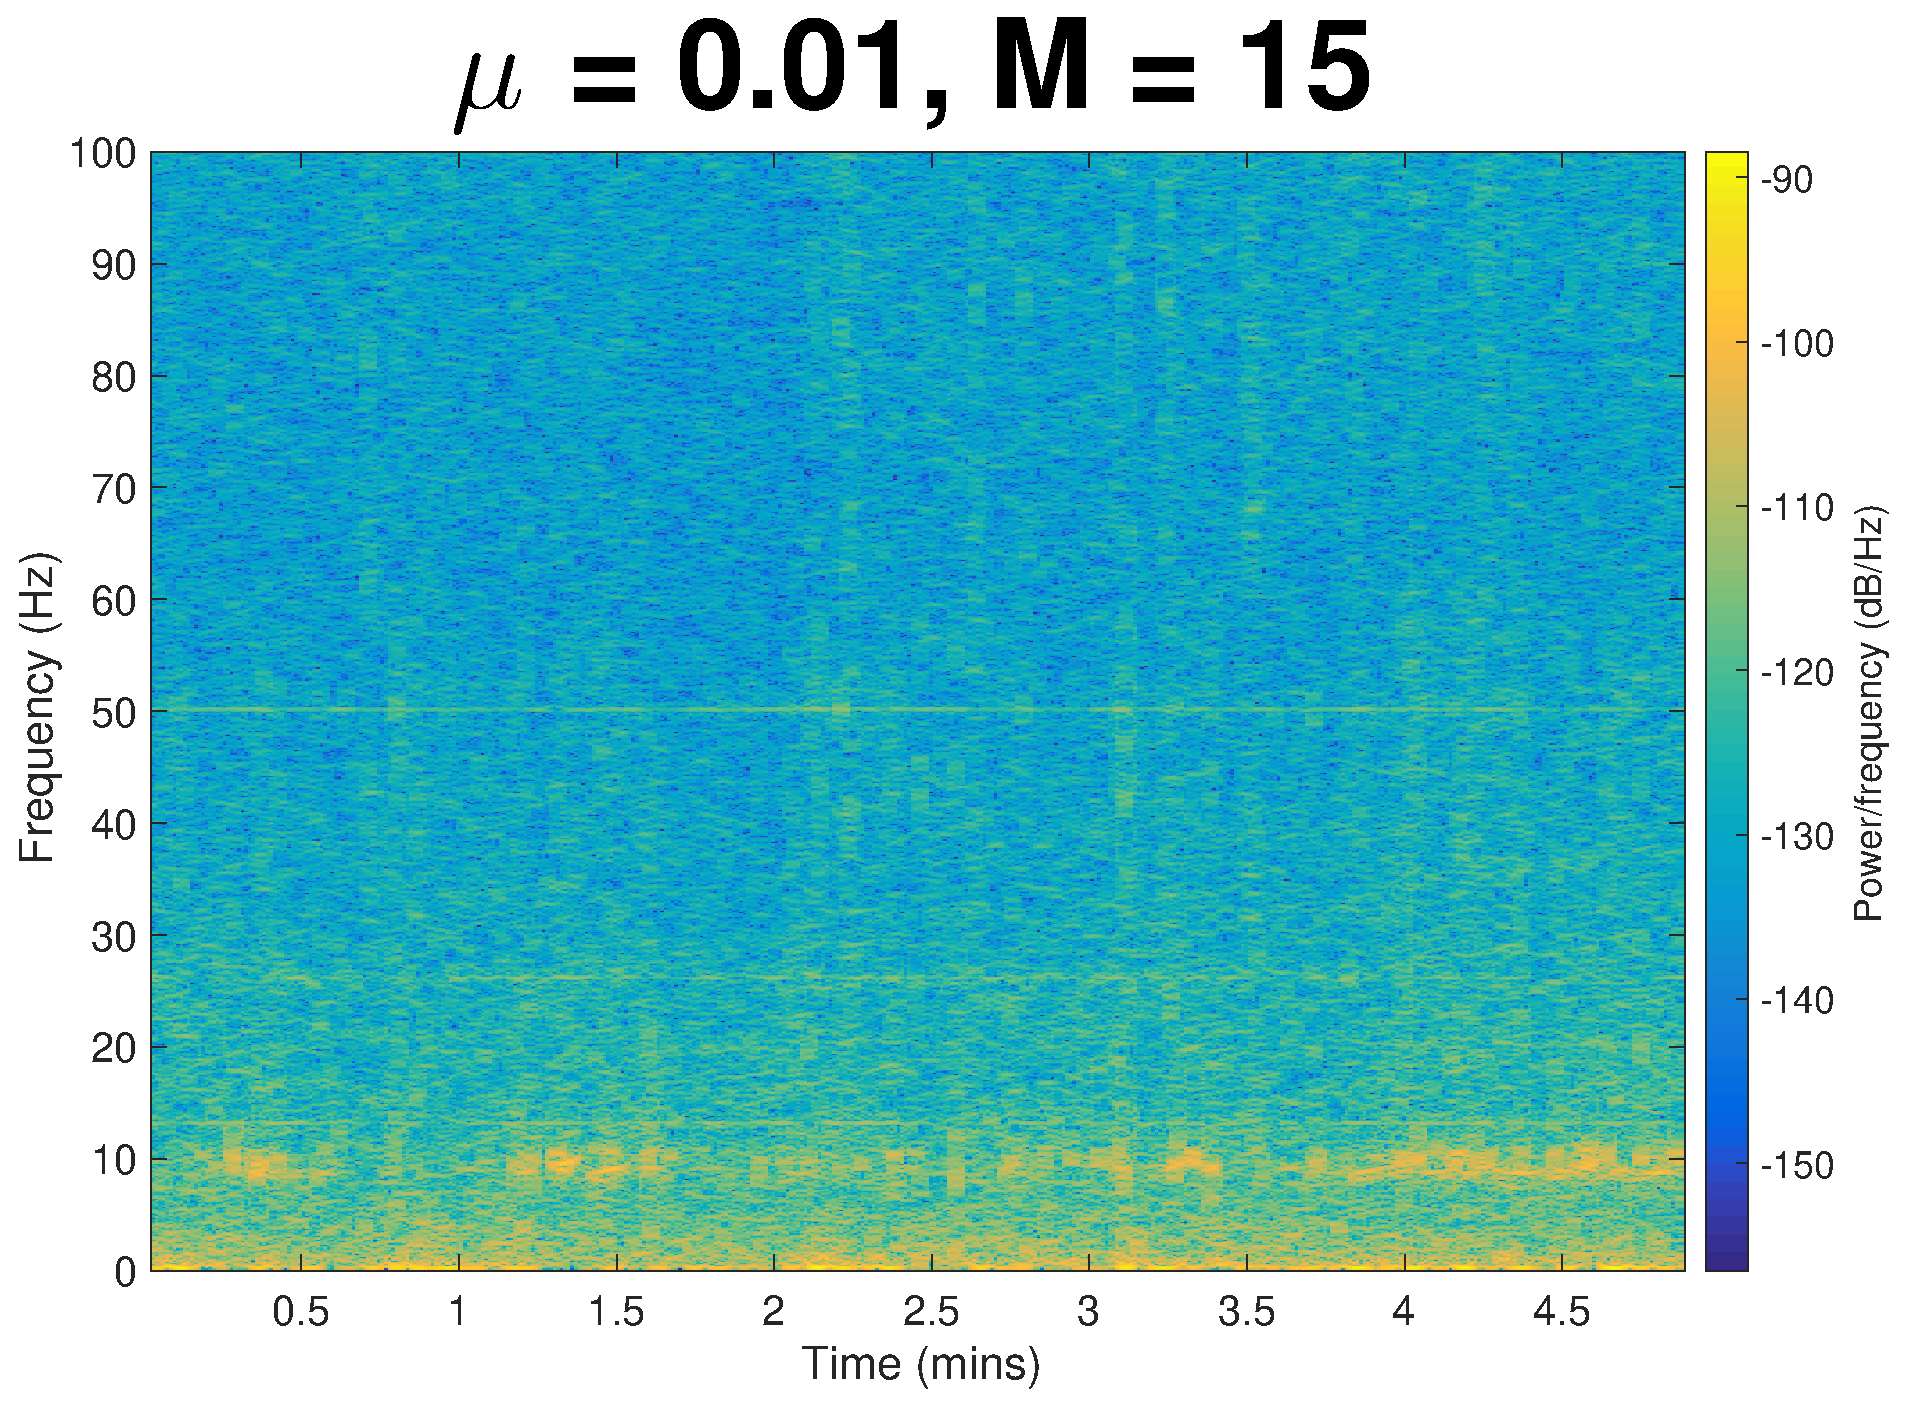
\includegraphics[width=0.24\textwidth]{part3/POz_mu_01_M_15}
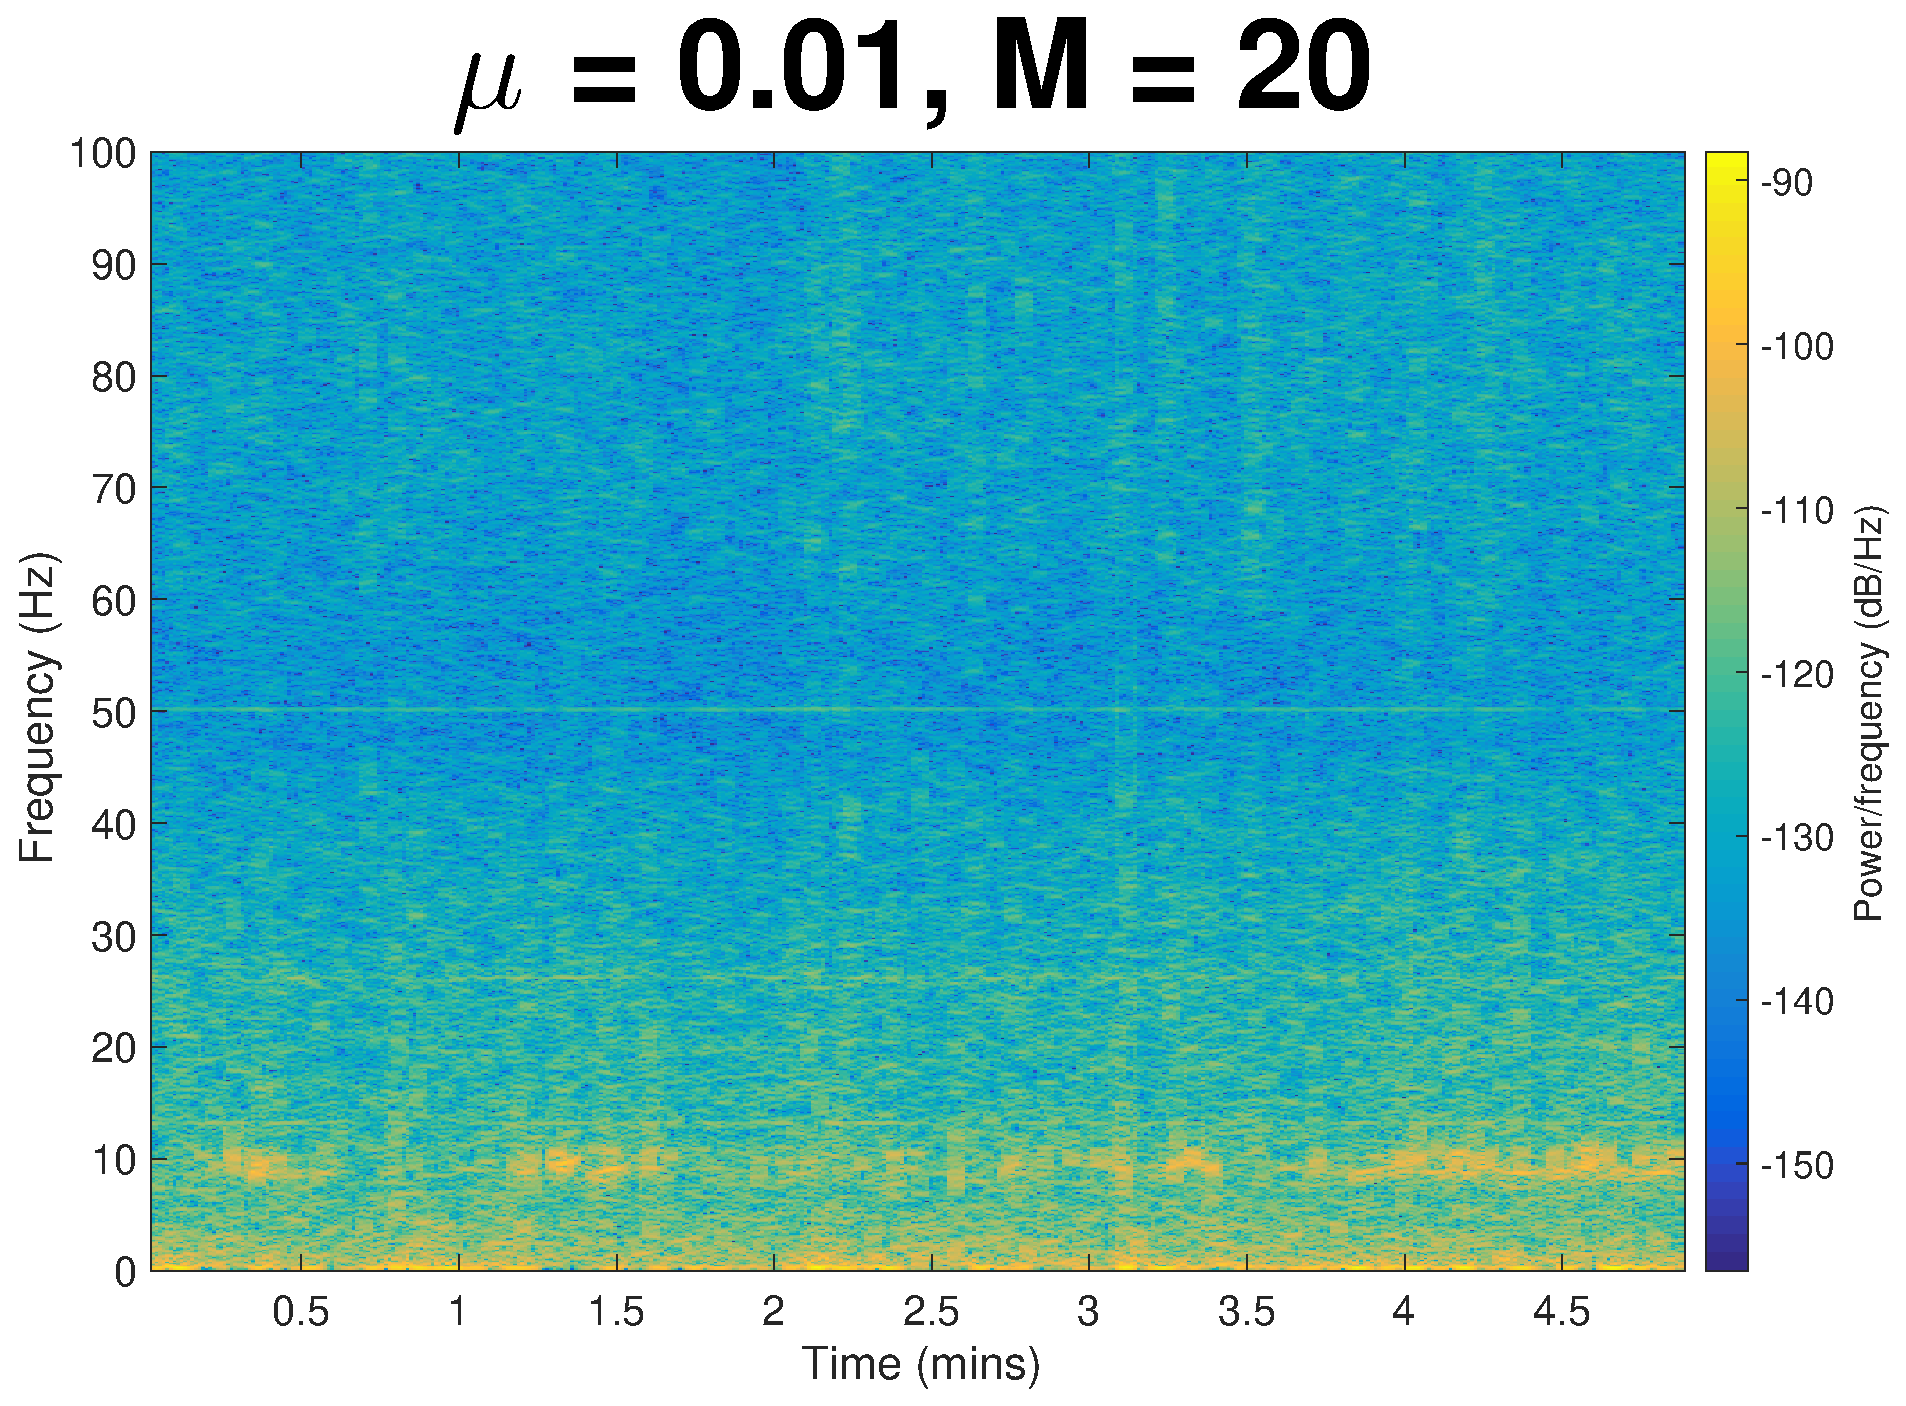
\includegraphics[width=0.24\textwidth]{part3/POz_mu_01_M_20}
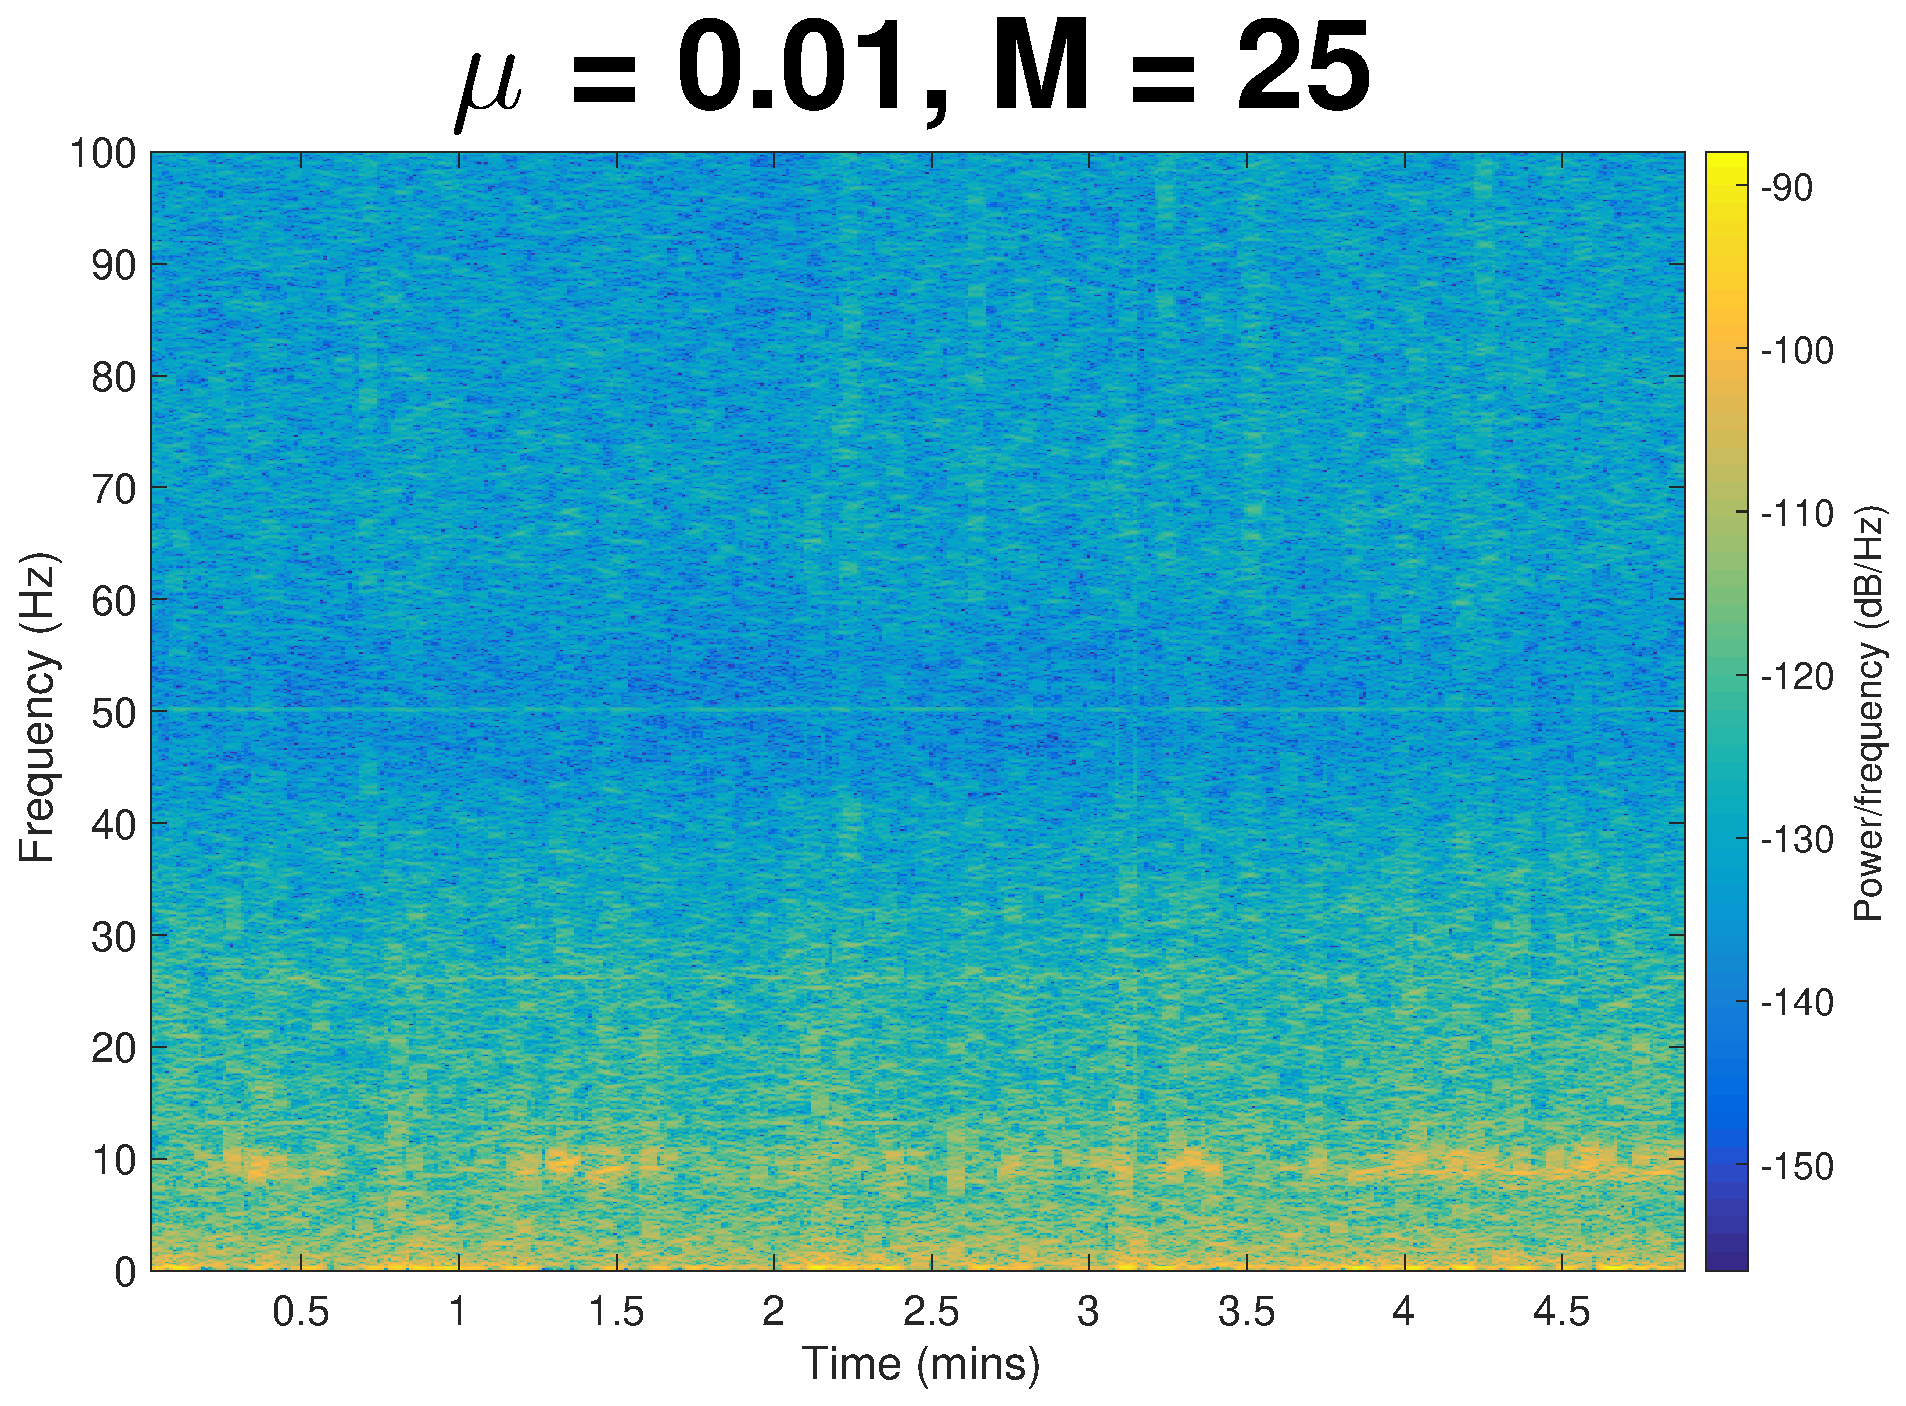
\includegraphics[width=0.24\textwidth]{part3/POz_mu_01_M_25}
\caption{Effect of Increasing Model Order on the Spectrogram of EEG Data}
\end{figure}

\begin{figure}[H]
\centering{}
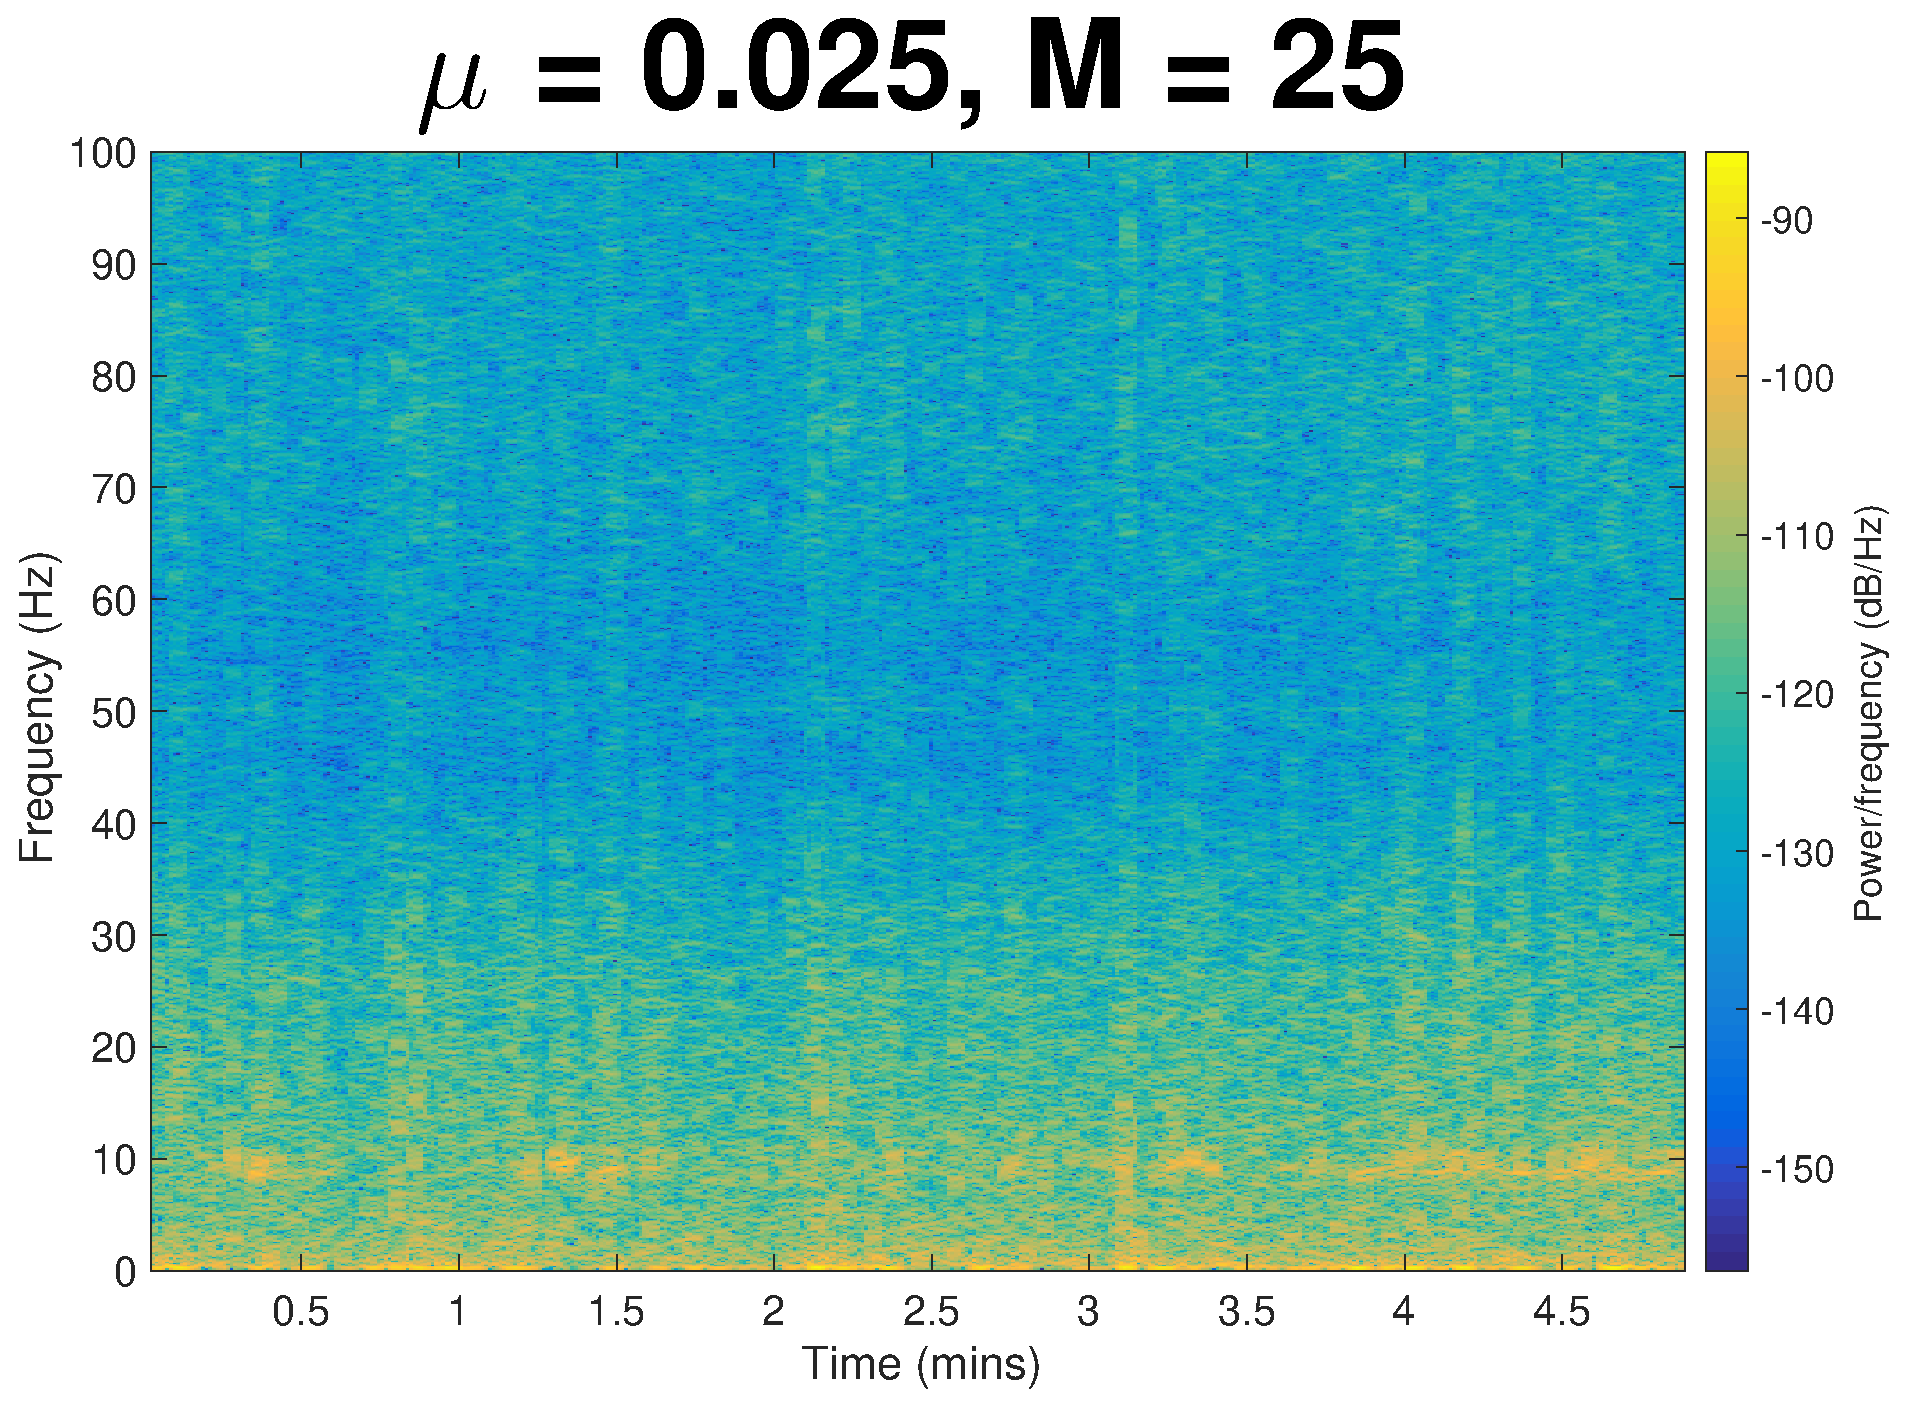
\includegraphics[width=0.24\textwidth]{part3/POz_mu_025_M_25}
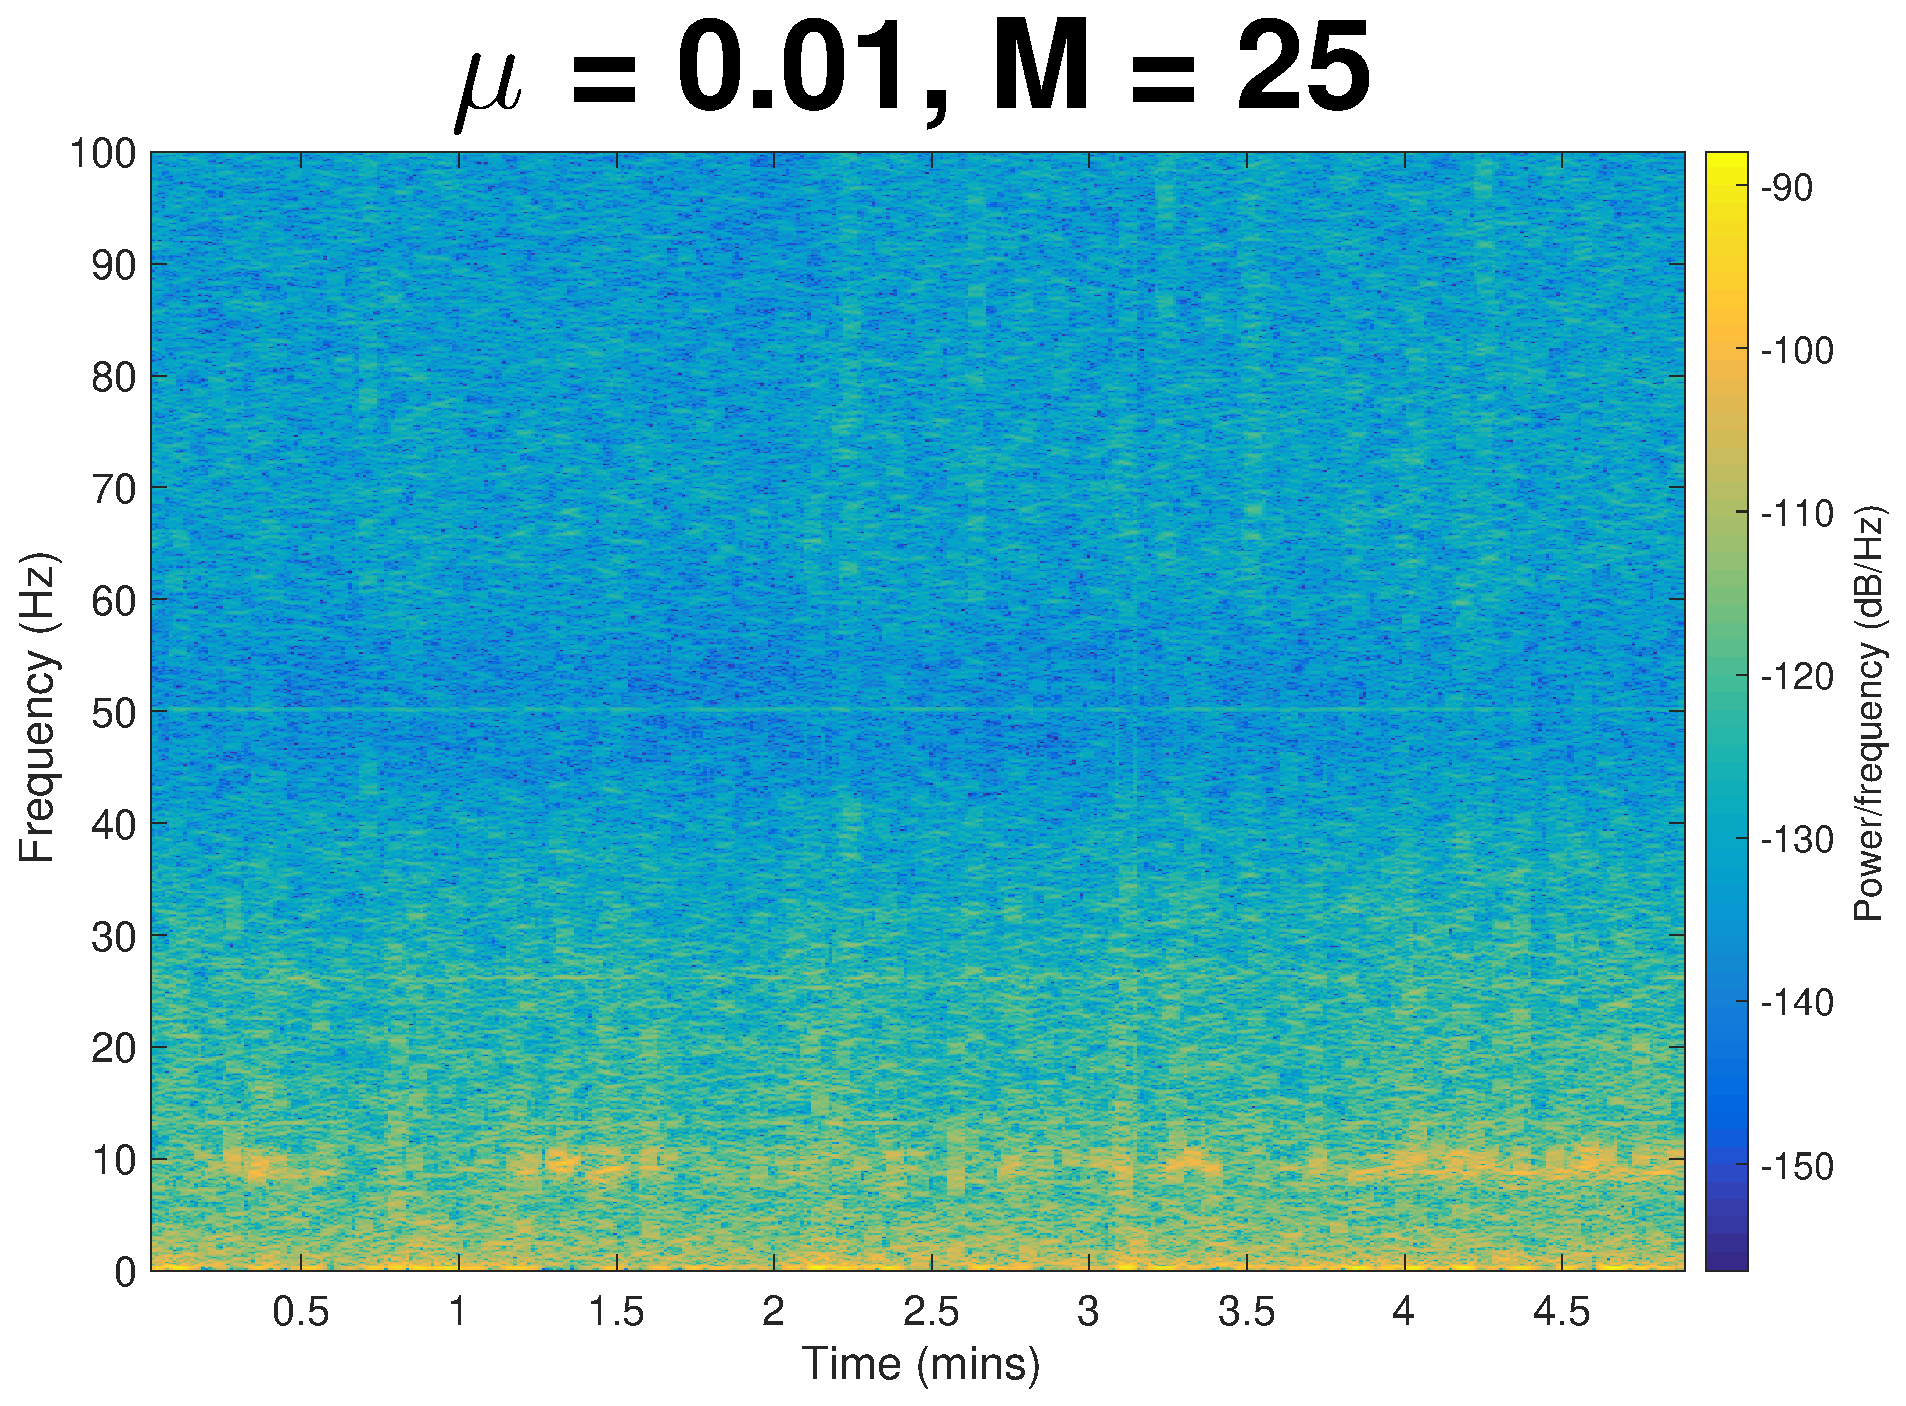
\includegraphics[width=0.24\textwidth]{part3/POz_mu_01_M_25}
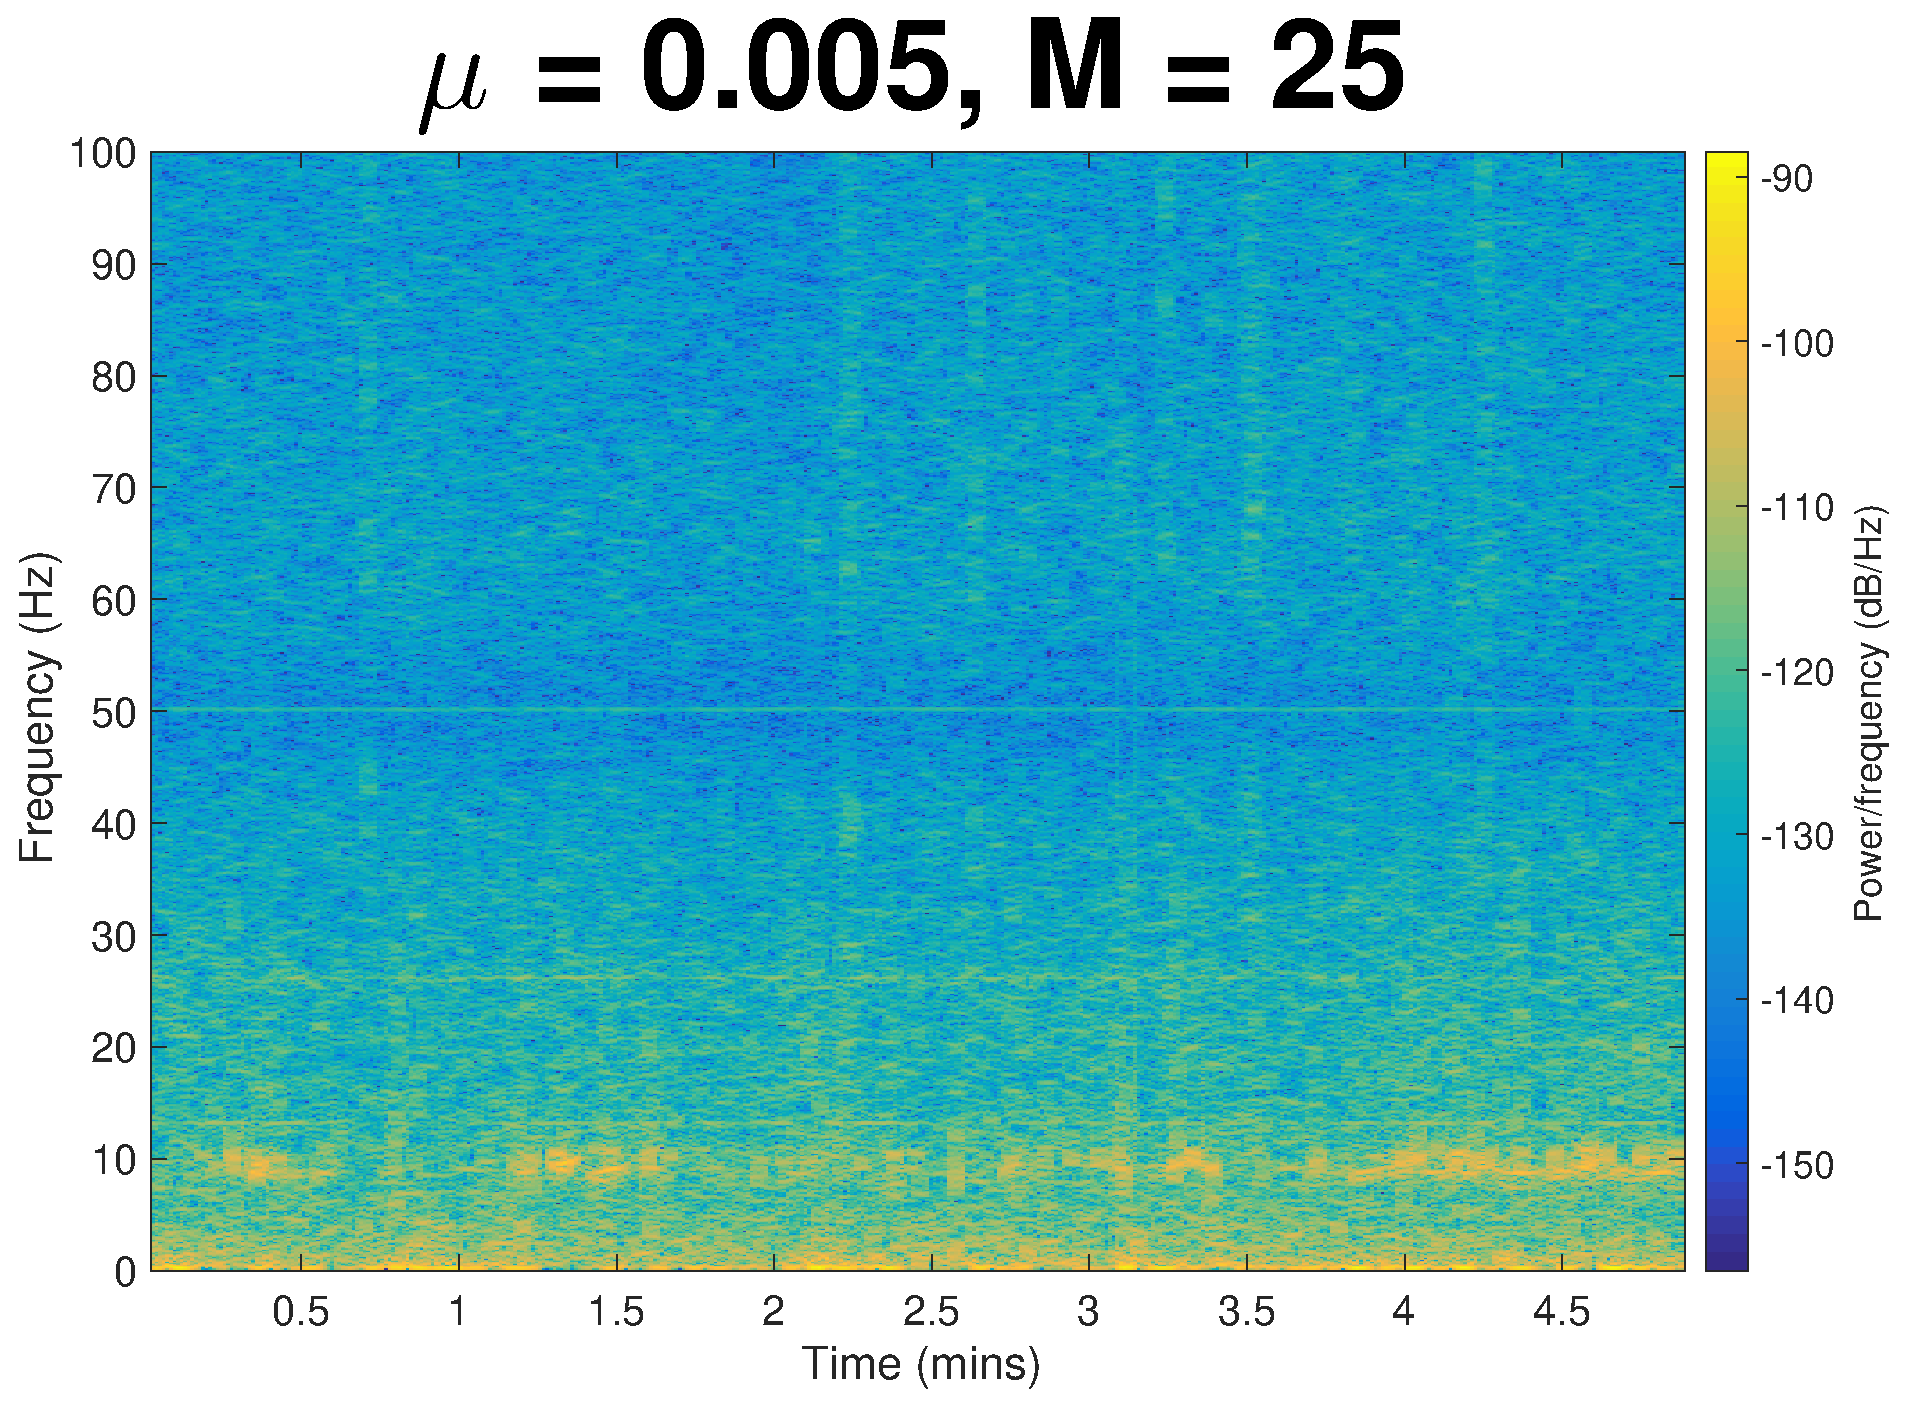
\includegraphics[width=0.24\textwidth]{part3/POz_mu_005_M_25}
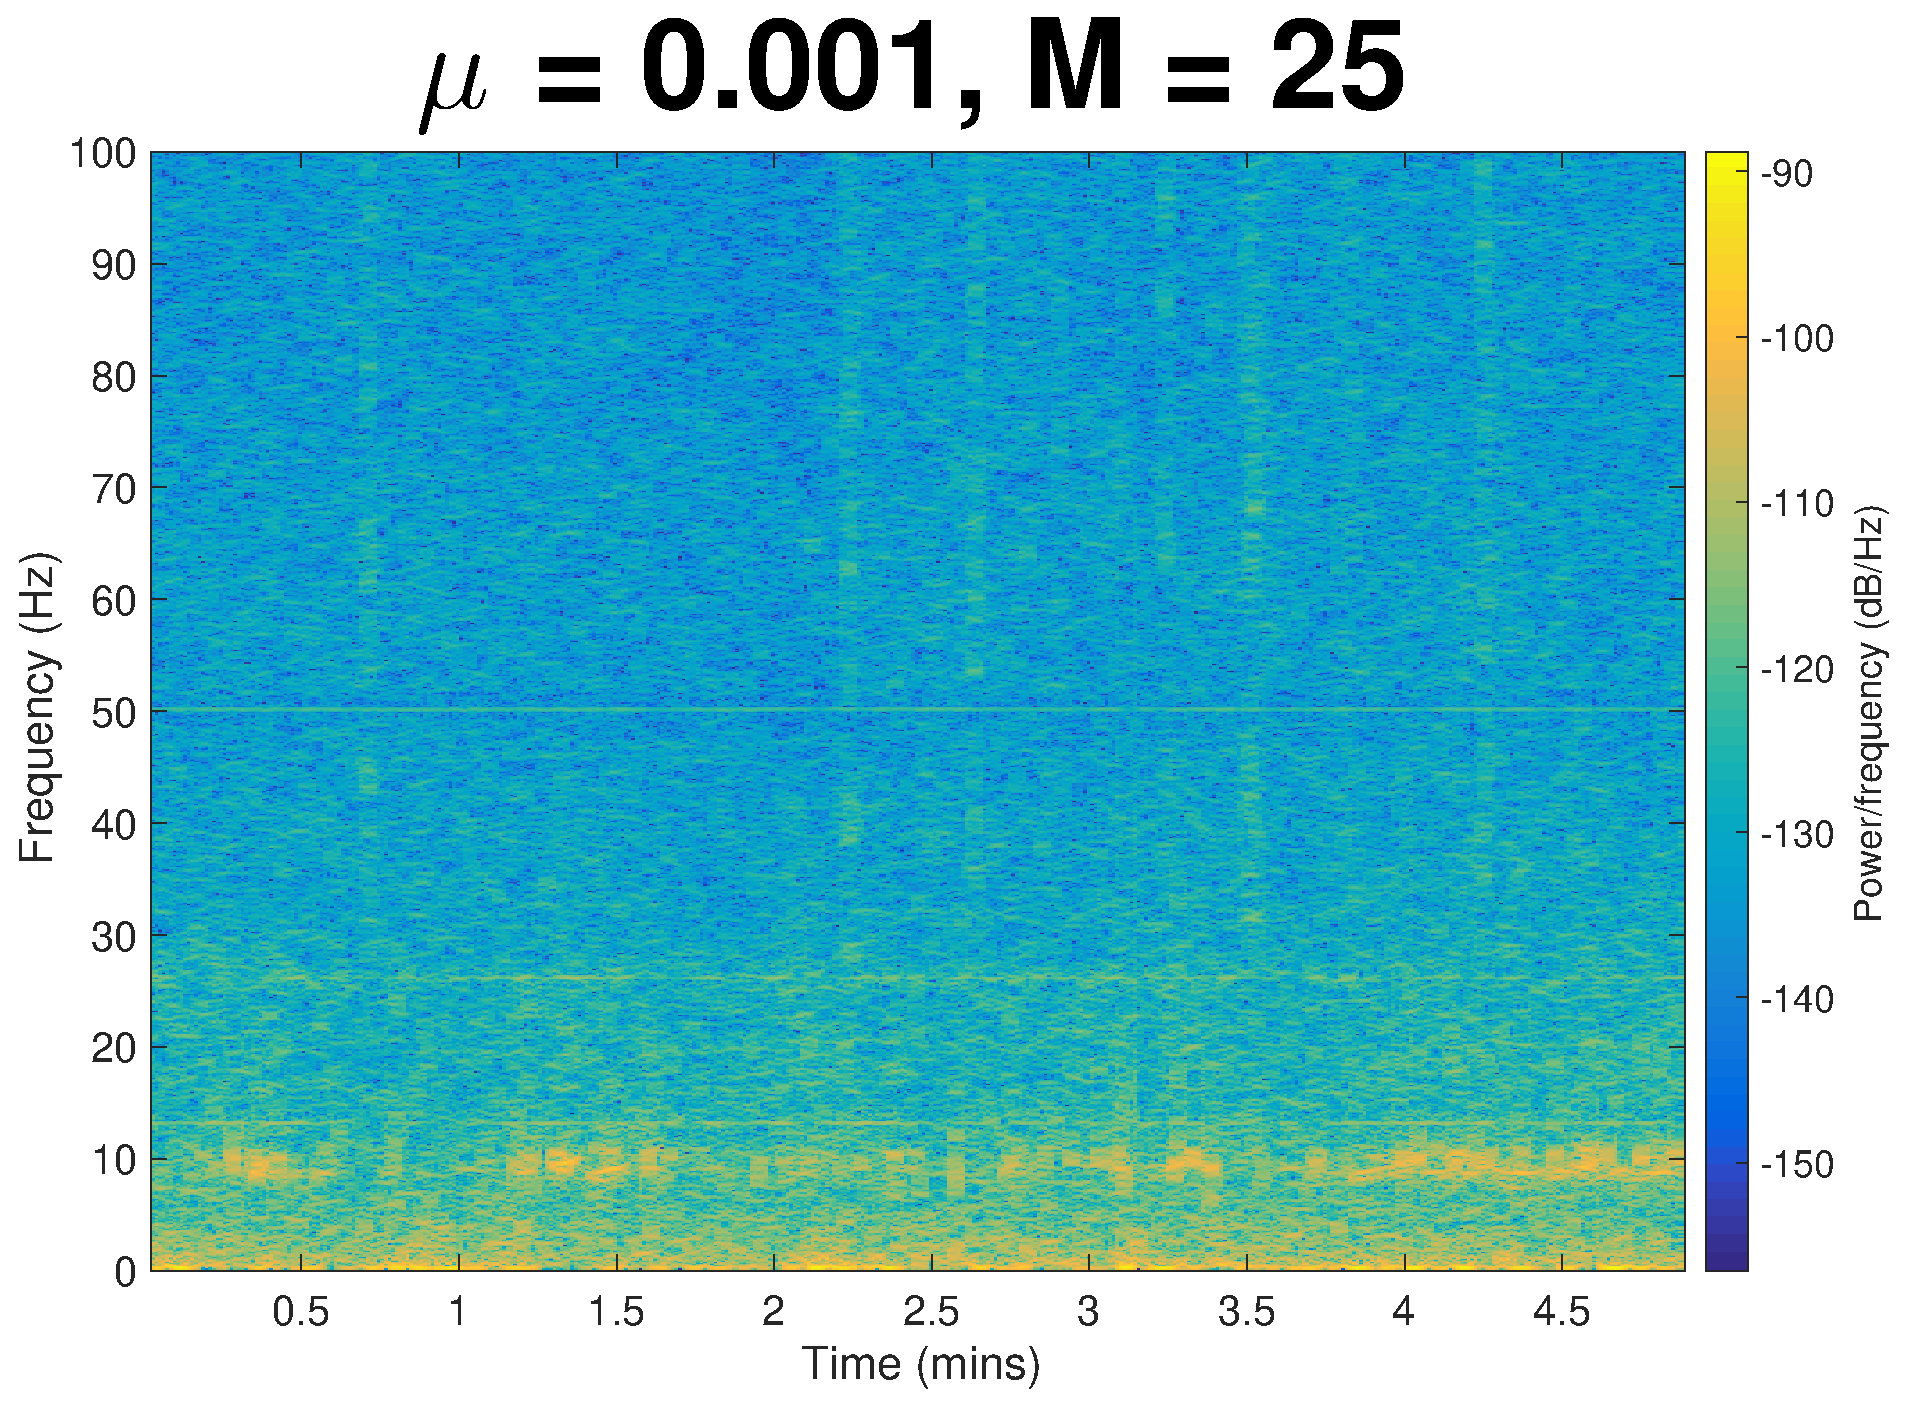
\includegraphics[width=0.24\textwidth]{part3/POz_mu_001_M_25}
\caption{Effect of Varying $\mu$ on the artifacts observed in the Spectrogram of Denoised EEG Data}
\end{figure}


\begin{figure}[H]
\centering{}
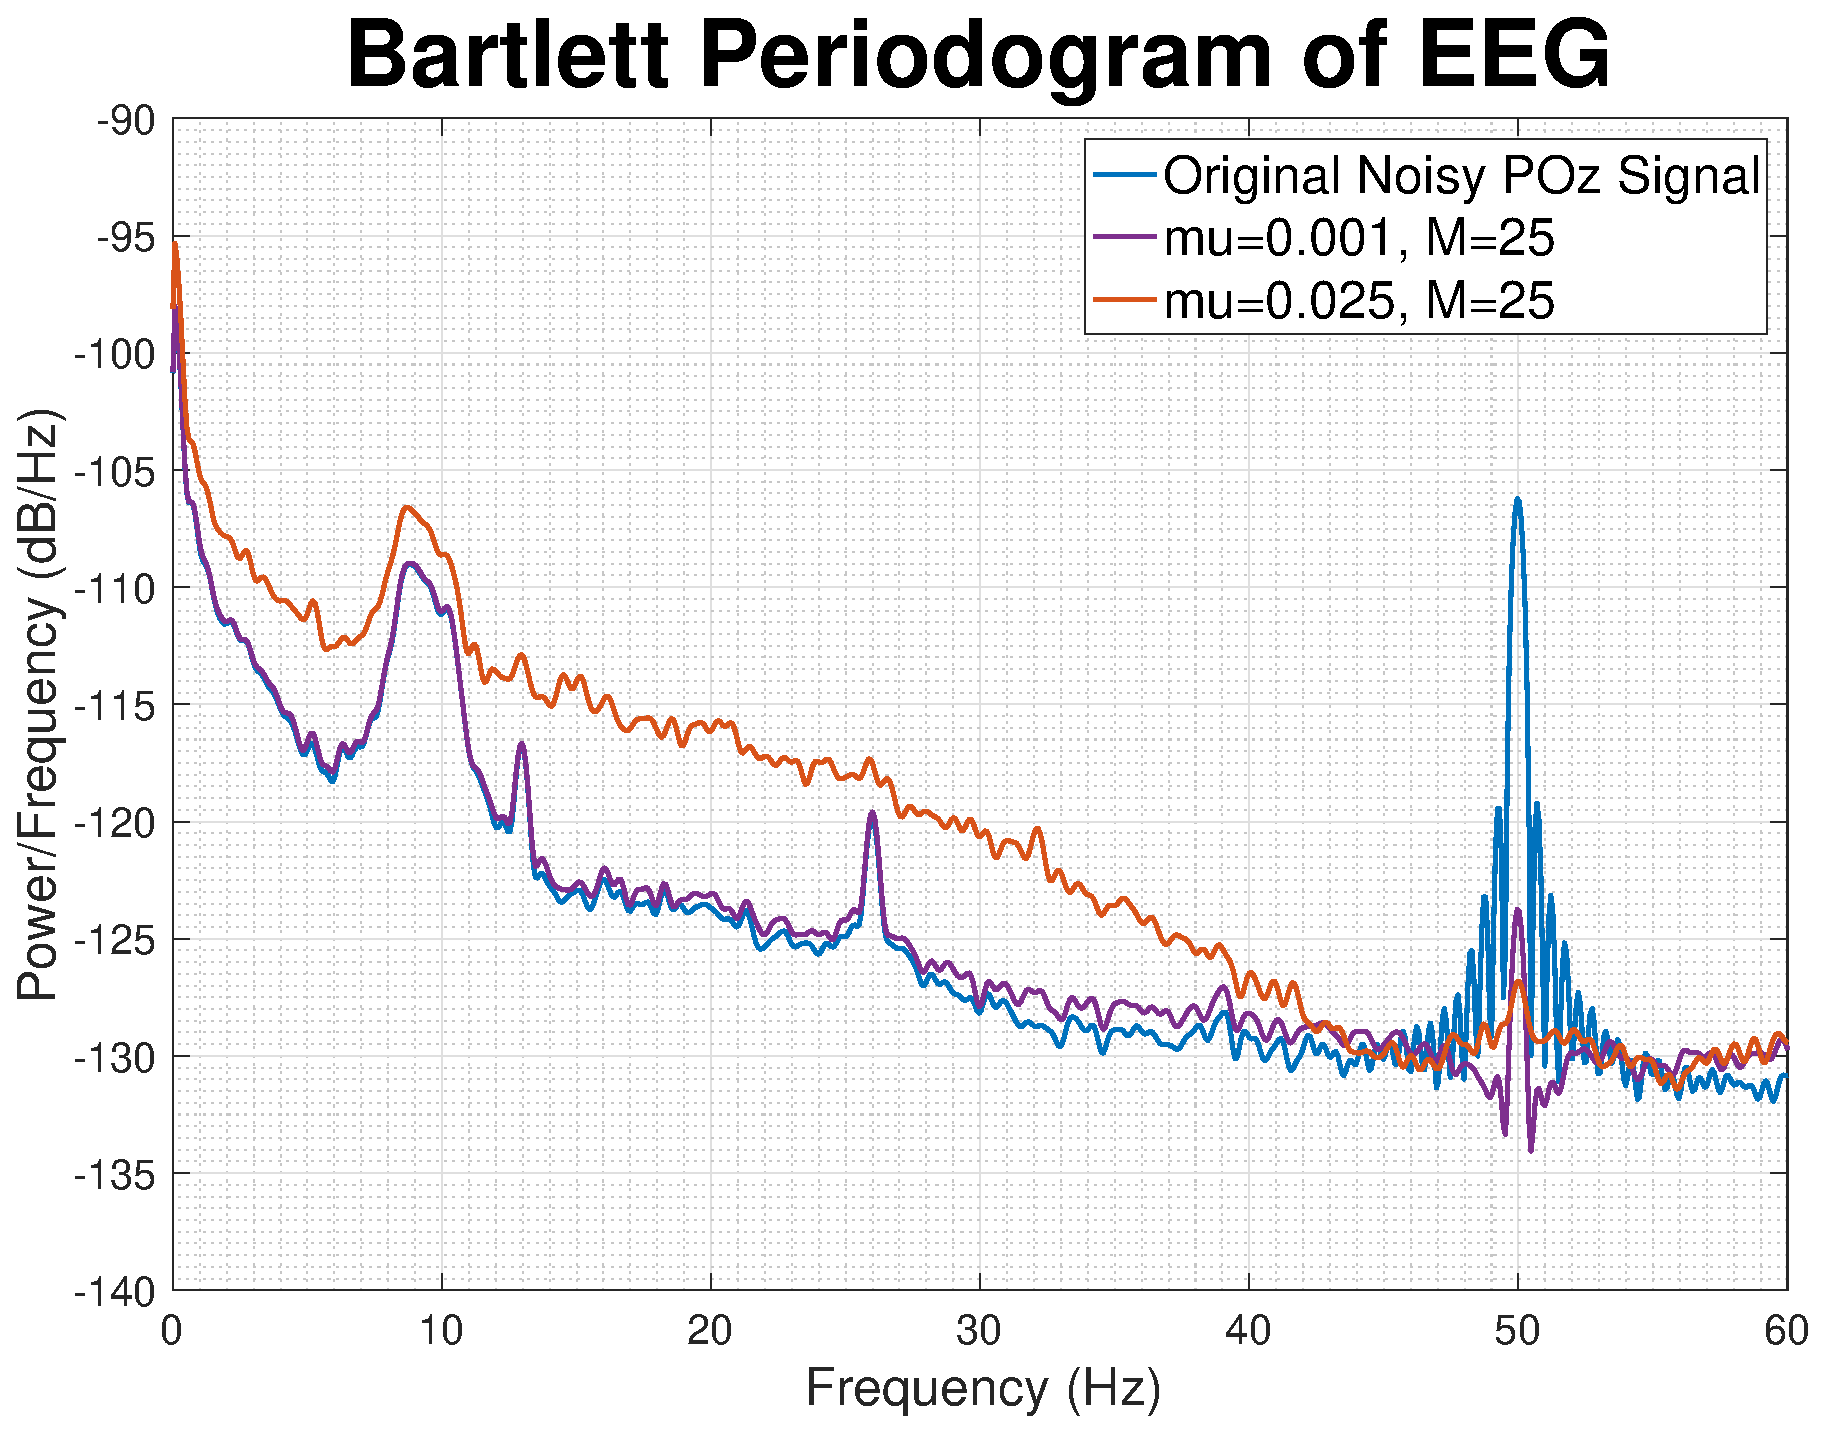
\includegraphics[width=0.32\textwidth]{part3/bartlett_cleaned_Poz}
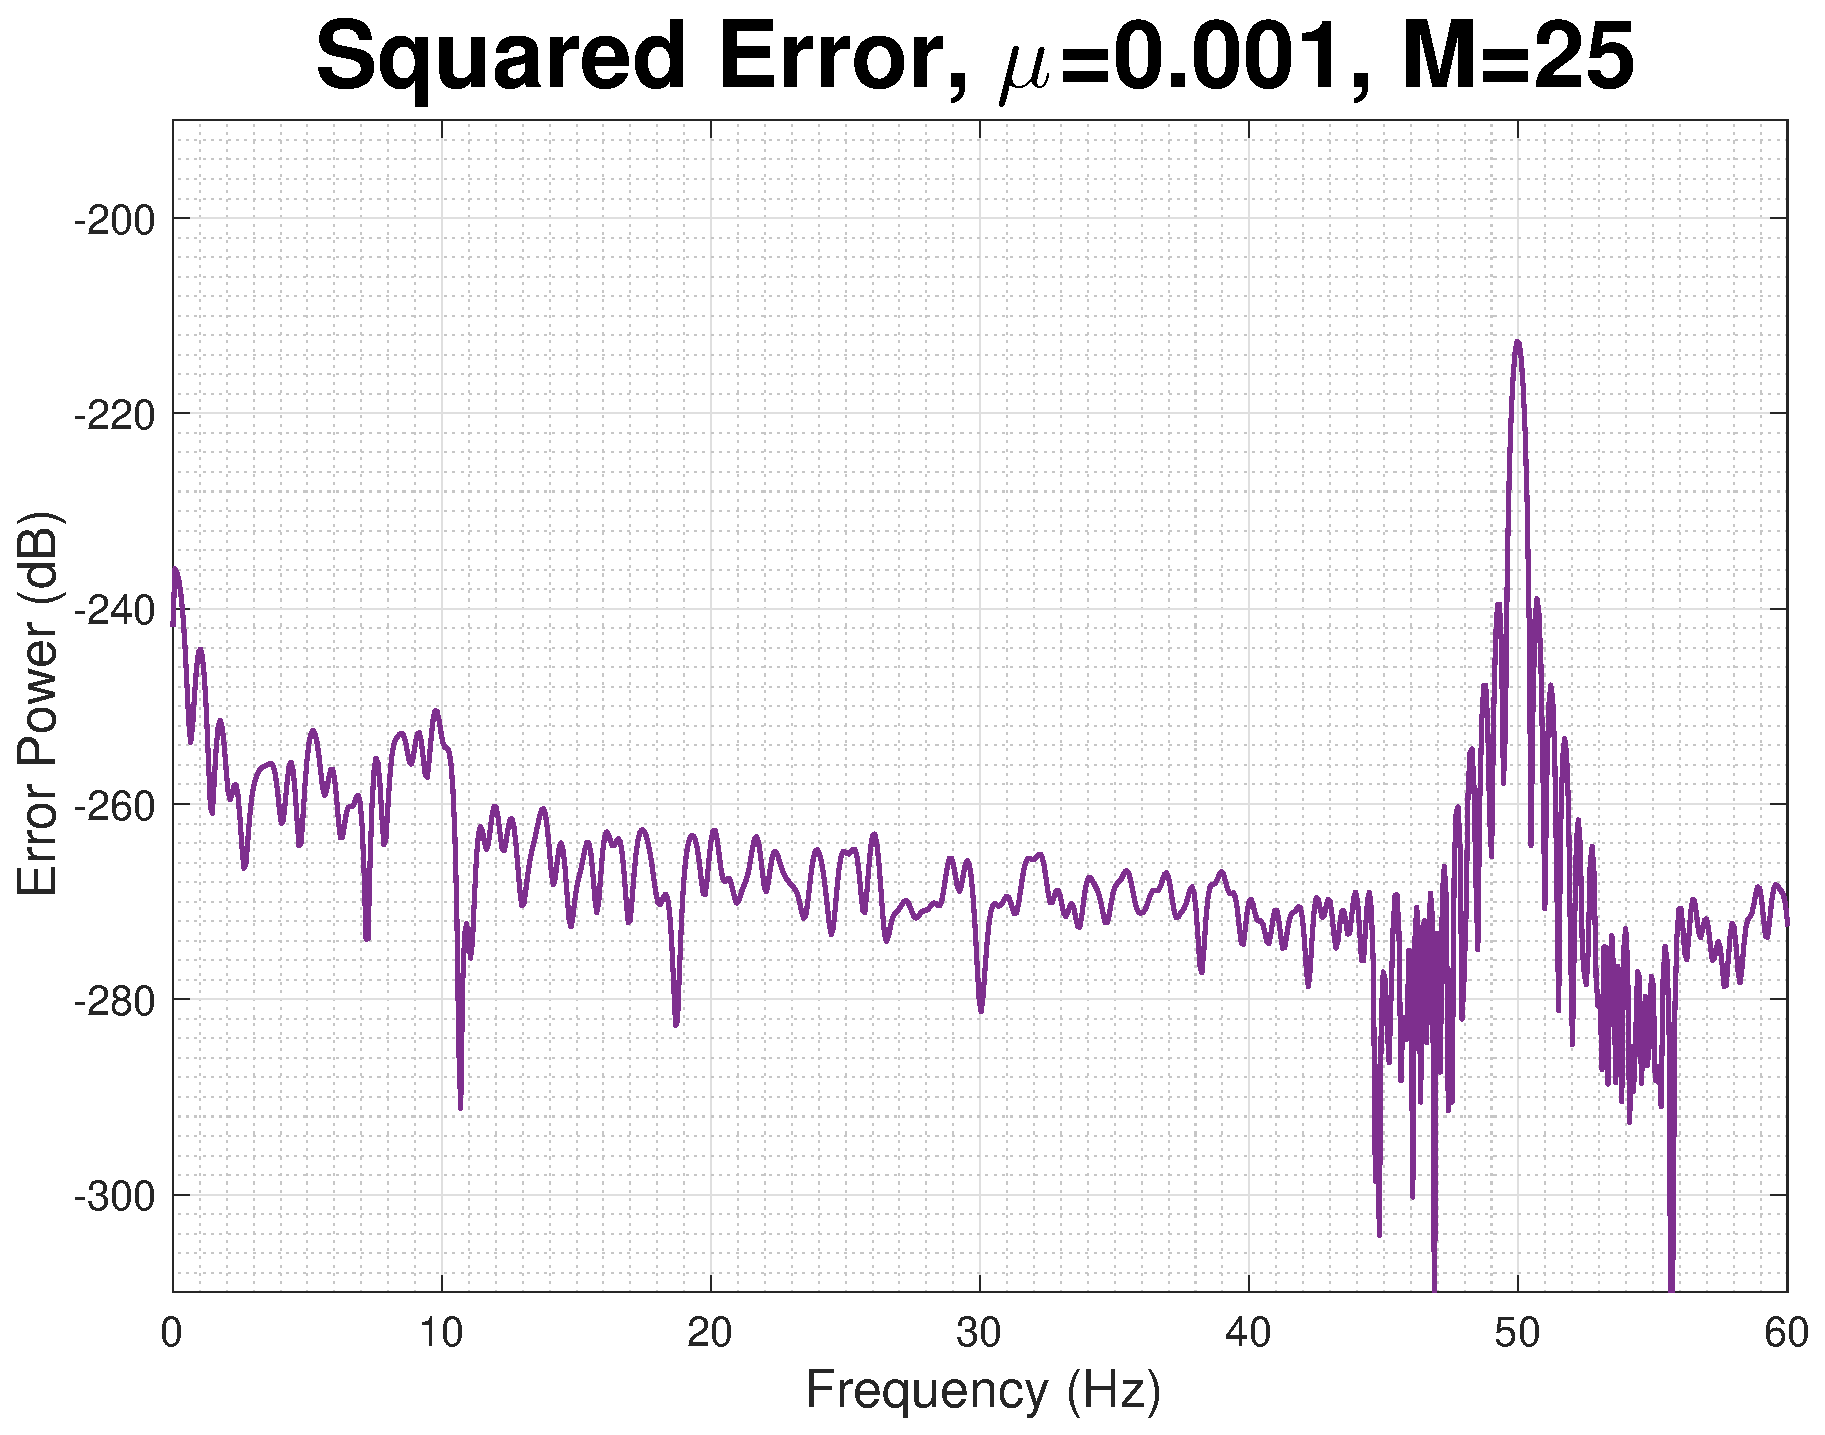
\includegraphics[width=0.32\textwidth]{part3/squared_error_periodogram}
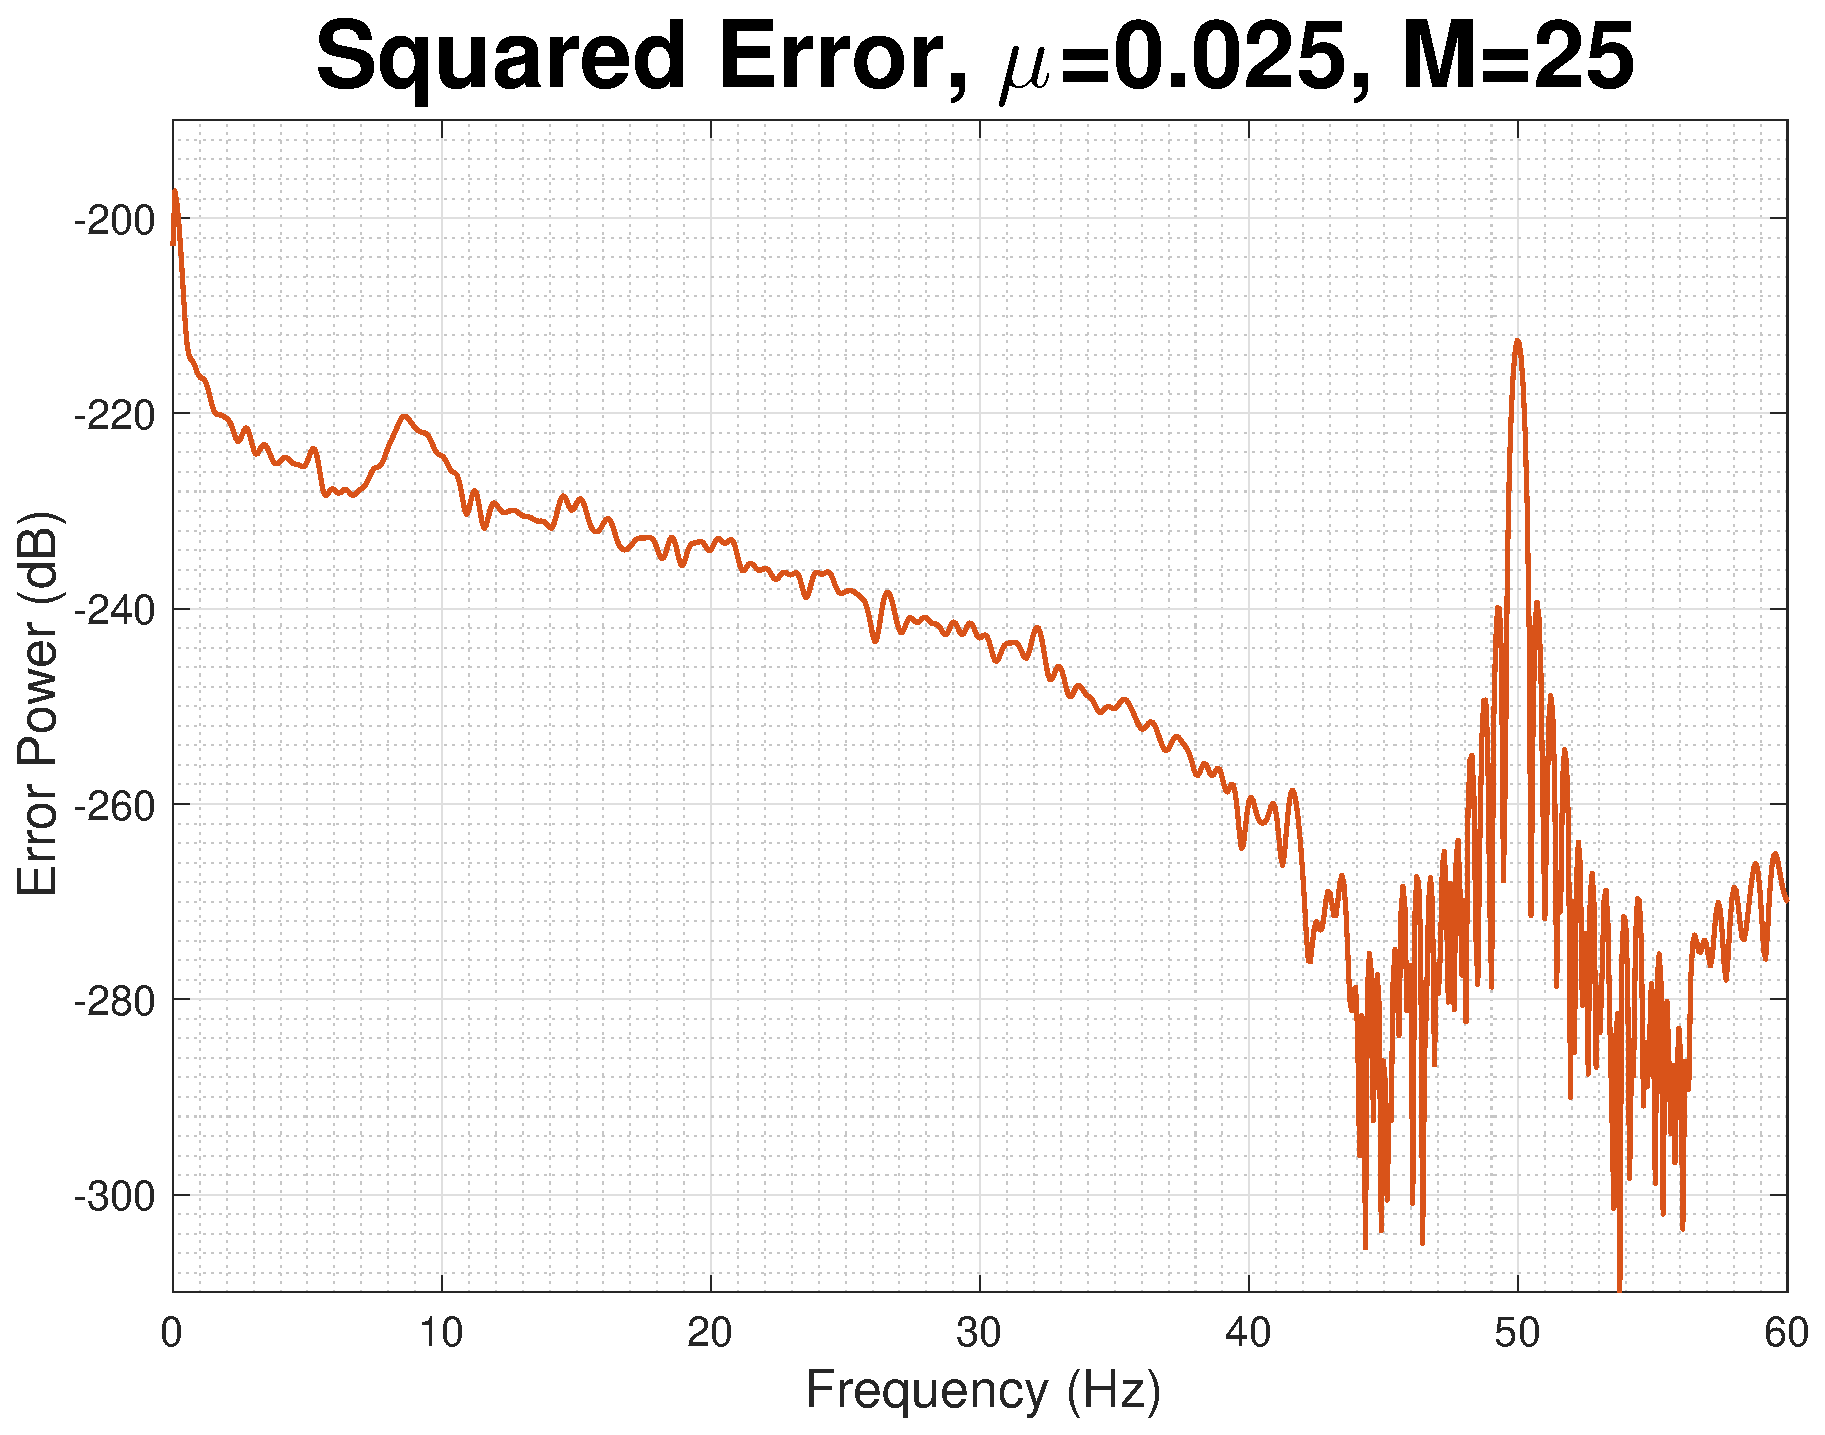
\includegraphics[width=0.32\textwidth]{part3/squared_error_periodogram_bad}
\caption{Bartlett Periodogram, averaged over 2 second intervals, and Squared Errors}
\end{figure}
